\documentclass[12pt,a4paper]{report}%{book}
\usepackage{emptypage}
\usepackage[shortlabels]{enumitem}
\usepackage[centertags]{amsmath}
\usepackage{amsfonts}
\usepackage{amssymb}
\usepackage{amsthm}
\usepackage{makecell}
\usepackage{graphicx}
\usepackage[table]{xcolor}
\usepackage{multirow}
\usepackage{tikz-cd} 
\usepackage{hhline}
%\usepackage{fontspec}
\usepackage{comment} %%%%%%%%%%%% pour un comentaire
\excludecomment{mycomment}
\usepackage{listings} % Package pour insérer du code
\lstset{language=Matlab}
\usepackage{xcolor} % Package pour la couleur
\usepackage{subcaption}
\usepackage{newlfont}
\usepackage{amsmath}
\usepackage{amssymb}
\usepackage{fontenc}
%\usepackage[francais]{babel}
\usepackage{fancyhdr} % Inclure le package fancyhdr
\usepackage{setspace}
\usepackage{pdfpages} %pour intégrer pdf
\usepackage{float}
\usepackage{color}
\usepackage{graphicx}
\usepackage{tabularx}
\usepackage[colorlinks=true,urlcolor=blue,linkcolor=blue!40!black,citecolor=blue]{hyperref}
%\usepackage{hyperref}   
\usepackage{ragged2e}
\usepackage{pgfplots}
\usepackage{graphicx}
\usepackage{bm}           
\usepackage{mathtools}   
\usepackage{mathrsfs}    
\usepackage{stmaryrd}
\usepackage{enumitem}
\usetikzlibrary{positioning, arrows.meta}
\usepackage{wallpaper}
\usepackage{changepage}
\usepackage{colortbl}
\usepackage{bmpsize}


%%%%%%%%%%%%%%%%%%%%%%%%%%%%%%%%%matlab%%%%%%%%%%%%%%%%%%
%\usepackage{listings}
%\lstset{language=Matlab}
%\usepackage[framemethod=tikz]{mdframed}
%\usetikzlibrary{matrix,fit,calc,arrows,shapes,positioning,shapes.callouts,arrows.meta,shadows.blur,backgrounds,decorations.text}


\usepackage[left=2cm,right=2cm,top=2cm,bottom=2cm]{geometry}

\usepackage{fancyhdr}
%\usepackage{pstricks}
\pagestyle{fancy}
\rhead{\thepage}
\lhead{\leftmark}
\rfoot{ Mohamed Najib LAATABI }      %%%%%%%% nome 
\lfoot{Faculté des Sciences de Rabat}
\renewcommand{\headrulewidth}{0.5mm}%la ligne de l'en tête du page 
\renewcommand{\footrulewidth}{0.5mm}
\pagestyle{fancy}
%\fancyhf{}
%\fancyfoot[C]{\fbox{\thepage}} % Encadre le numéro de page au centre du pied de page
\fancyfoot[C]{\fcolorbox{chapname}{white}{\textcolor{chapname}{\thepage}}} 


\usepackage{tikz}
\usepackage[french]{babel}
\usepackage{fancyhdr}
\usepackage{graphicx}
\usepackage{calc}
  \usepackage{fancybox}
\usepackage{xcolor}
\usepackage[utf8]{inputenc}
%\usepackage[top=1cm,bottom=1cm,right=1cm,left=1cm]{geometry}
\usepackage{amsmath,amsfonts,amssymb,mathrsfs}
\usetikzlibrary{calc}
\tikzstyle{a} = [rectangle,draw=black,line width=1mm,minimum size=1cm]
\def\siz{0.75}
\setstretch{1.1}%pour espace entre les ligne


%%%%%%%%%%%%%%%%%%%%%%%%%%%%%%%%%%%%%%%%%%%style chapitre%%%%%%%%%

\usepackage[explicit]{titlesec}

\usepackage{lmodern}% to have a large font size for the chapter numbers


\definecolor{chapnumberbg}{RGB}{26,40,105}
\definecolor{chapname}{RGB}{100,117,158}

\titleformat{\chapter}[display]
  {\normalfont}
  {}
  {0pt}
  {%
    \begin{tikzpicture}
    \node[
      draw=chapname,
      rounded corners,
      outer sep=0pt,
      inner sep=6pt,
      rotate=90,
      line width=1pt,
      font=\Large\color{chapnumberbg}\bfseries
      ]
      (chapname) 
      {\chaptertitlename};
    \node[
      fill=chapnumberbg,
      minimum width=2cm,
      minimum height=2.3cm,
      rounded corners,
      anchor=west,
      font=\color{white}\fontsize{40}{48}\selectfont\bfseries
      ]
      at ([xshift=6pt]chapname.south)
      (chapnumber)
      {\thechapter};
    \node[
      anchor=west,
      text width=\textwidth-4cm,
      font=\bfseries\LARGE
      ] 
      at ([xshift=10pt]chapnumber.east)
      {#1};
    \fill[
      overlay,
      draw=none,
      line width=0pt,
      rounded corners=1pt,
      left color=chapnumberbg,
      right color=chapnumberbg!10
      ]
      ([yshift=-3pt]chapname.north west) rectangle ++(\textwidth,-3pt);  
    \end{tikzpicture}%
  }
\titleformat{name=\chapter,numberless}[display]
  {\normalfont}
  {}
  {0pt}
  {%
    \begin{tikzpicture}
    \node[
      anchor=west,
      inner sep=0pt,
      outer sep=0pt,
      text width=\textwidth,
      font=\bfseries\LARGE
      ]
      (chaptitle) 
      {#1};
    \fill[
      overlay,
      draw=none,
      line width=0pt,
      rounded corners=1pt,
      left color=chapnumberbg,
      right color=chapnumberbg!10
      ]
      ([yshift=-3pt]chaptitle.south west) rectangle ++(\textwidth,-3pt);  
    \end{tikzpicture}%
  }

 %%%%%%%%%%%%%%%%%%%%%%%%%%%%%%%%%%%%%%%%%%%%%%%%%%%%%%%%%%% Définition de la nouvelle commande \R
\newcommand{\R}{\mathbb{R}}
\newcommand{\B}{\mathbb{B}(\mathbb{R})}
\newcommand{\Bn}{\mathbb{B}(\mathbb{R}^n)}

%%%%%%%%%%%%%%%%%%%%%%%%%%%%proof Démonstration %%%%%%%%%%%%%%%%%%%%%%%%%%%%%%%%%%%%%%%%%
\renewcommand{\qedsymbol}{\textcolor{black}{\ensuremath{\blacksquare}}}

%%%%%%%%%%%%%%%%%%%%%%%%%%%%%%%%%%%%%%Definition%%%
\newcounter{definition}[section] % Créer un compteur pour les définitions
\counterwithin{definition}{section} % Lier le compteur de définition au compteur de section
\usepackage[tikz]{bclogo}
  \usepackage{bclogo}
  \usepackage[many]{tcolorbox}
\usepackage{tcolorbox}
%%%%%%%%%%%%%%%%%%%%%%%%%%%%%%%%%%\definecolor{gainsboro}{rgb}{0.86, 0.86, 0.86}
\newenvironment{définition}[2][]
  {\refstepcounter{definition}% Incrémenter le compteur
  \begin{bclogo}[
    logo=\bcplume,
    couleur=blue!6,    %%%%%%%%%cyan!10,
    arrondi=0.1,
    couleurBord=white,#1]{Définition \thedefinition :#2}
  }
  {\end{bclogo}}
%%%%%%%%%%%%%%%%%%%%%%%%%%%%%%%%%%%%%%%%%%%%Proposition
  \newcounter{proposition}[section] % Créer un compteur pour les définitions
\counterwithin{proposition}{section} % Lier le compteur de définition au compteur de section
 \newenvironment{Proposition}[2][]
  {\refstepcounter{proposition}% Incrémenter le compteur
  \begin{bclogo}[
    logo=\bcplume,
    couleur=aliceblue,
    arrondi=0.1,
    barre = snake ,
    couleurBord=white,#1]{Proposition \theproposition: #2}
  }
  {\end{bclogo}}
 \definecolor{aliceblue}{rgb}{0.94, 0.97, 1.0}


%%%%%%%%%%%%%%%%%%%%%%%%%%%%%%%%%%%%%%%%%%%Propriété
\newcounter{Prop}[section] % Créer un compteur pour les définitions
\counterwithin{Prop}{section} % Lier le compteur de définition au compteur de section
 \newenvironment{Propriété}[2][]
  {\refstepcounter{Prop}% Incrémenter le compteur
  \begin{bclogo}[
    logo=\bcplume,
    couleur=aliceblue1,
    arrondi=0.1,
    barre = snake ,
    couleurBord=white,#1]{Propriété \theProp: #2}
  }
  {\end{bclogo}}
    \definecolor{aliceblue1}{rgb}{0.94, 0.97, 1.0}

 
   %%%%%%%%%%%%%%%%%%%%%%%%%%%%%%%%%%%%%%%%%Remarque & Exemple
\newcounter{remm}[chapter]

 \newenvironment{remarque}[2][]
  {\refstepcounter{remm}
  \begin{bclogo}[
    %logo=\bctakecare,
    couleur=white,
    arrondi=0.1,
    couleurBord=white,#1]{Remarque \theremm:#2}
  }
  {\end{bclogo}}

\newcounter{PP}[chapter]  
   \newenvironment{exemple}[2][]
  {\refstepcounter{PP}
  \begin{bclogo}[
    logo=\bccrayon , % \bclampe,
    couleur=white,
    arrondi=0.1,
    barre =snake,
     tailleOndu = 1.5,
    couleurBord=white,#1]{Exemple \thePP:#2}
  }
  {\end{bclogo}}
%%%%%%%%%%%%%%%%%%%%%%%%%%%%%%
%%%%%%%%%%%%%%%%%%%%%%%%%%%corollaire
  \newcounter{corollaire}[section] % Créer un compteur pour les définitions
\counterwithin{corollaire}{section} % Lier le compteur de définition au compteur de section
 \newenvironment{corollaire}[2][]
  {\refstepcounter{corollaire}% Incrémenter le compteur
  \begin{bclogo}[
    logo=\bcplume,
    couleur=aliceblue2,
    arrondi=0.1,
    barre = snake ,
    couleurBord=white,#1]{Corollaire \thecorollaire: #2}
  }
  {\end{bclogo}}
    \definecolor{aliceblue2}{rgb}{0.97, 0.97, 1.0}%{0.96, 1.0, 0.98}
%%%%%%%%%%%%%%%%%Lemma
  \newcounter{lemma}[section] % Créer un compteur pour les définitions
\counterwithin{lemma}{section} % Lier le compteur de définition au compteur de section
% Incrémenter le compteur

    \newenvironment{lemme}[2][]
  {\refstepcounter{lemma}
  \begin{bclogo}[
    logo=\bccle,
    couleur=mintcream1,
    arrondi=0.1,
    couleurBord=white,#1]{Lemme \thelemma:#2}
  }
  {\end{bclogo}}
 \definecolor{mintcream1}{rgb}{0.95, 0.95, 0.96}%{0.86, 0.86, 0.90}
  \definecolor{mintcream}{rgb}{0.96, 1.0, 0.98}
%%%%%%%%%%%%%%%%%%%%%%%
  \definecolor{mintcream}{rgb}{0.96, 1.0, 0.98}
%%%%%%%%%%%%%%%%%%%%%%%%%%%%%%%%%%%%%Theoreme%%%%%%%%%%%%%%%%%%%%%%%%
\definecolor{ceruleanblue}{rgb}{0.86, 0.86, 0.86}%{0.63,0.79, 0.95}             %%%%%%%{0.16, 0.32, 0.75}  pour le titre               
	\definecolor{mintcream}{rgb}{0.96, 0.96, 0.96}% {0.96, 1.0, 0.98}
	\definecolor{arsenic}{rgb}{0.96, 1.0, 0.98}%{0.23, 0.27, 0.29}
%\newtcolorbox[auto counter,number within=section,number format=\arabic,list inside=mytheorems]{theorembox}[2][]{lower separated=false,colback=blue!6!white,colframe=black!50,fonttitle=\bfseries\upshape,fontupper=\slshape,colbacktitle=ceruleanblue,coltitle=black,enhanced,attachboxed title to top left={yshift=-0.1in,xshift=0.10in}, boxed title style={boxrule=1pt,colframe=black!50,},title=Théorème \thetcbcounter: #2, #1}

%\newenvironment{théorème}[1][]{%
% \begin{theorembox}[#1]
%}{%
 %   \end{theorembox}
%}

%%%%%%%%%%%%%%%%%%%%%%%%%%%%%%%%%%%%%%%%%%%%%%%%%%%%%%%%%%%%%%%%%%%%%%%%%%%%%%%%%%the
\newtcbtheorem[auto counter,number within=section]{théorème}%
  {Théorème}{fonttitle=\bfseries\upshape, fontupper=\slshape,
     arc=0mm, colback=blue!5!white,colframe=myblue}{theorem}
  
  %%%%%%%%%%%%%%%%%%%%%%%%%%%%%%%%%%%%%%%%%%%%%%%%%5% colors===========================================
  \definecolor{lightmauve}{rgb}{0.97, 0.96, 1.0}
\definecolor{mybluei}{RGB}{5, 0, 100}
\definecolor{myblueii}{RGB}{0, 0, 100}
\definecolor{mybluei2}{RGB}{0,173,239}
\definecolor{myblueii2}{RGB}{63,200,244}
\definecolor{myblueiii}{RGB}{199,234,253}
\definecolor{myblue}{RGB}{0,82,155}
\definecolor{mybluei3}{RGB}{0,173,239}
\definecolor{winered}{rgb}{0.5,0,0}
\definecolor{bule}{RGB}{18,29,57}
\definecolor{doc}{RGB}{0,60,110}
\definecolor{denim}{rgb}{0.08, 0.38, 0.74}
\definecolor{ufla_blue}{HTML}{224271} 
\definecolor{chaptercolor}{rgb}{0.36,0.73,0.82}
\definecolor{MainRed}{rgb}{.6, .1, .1}
\definecolor{GoldDecoration}{RGB}{170, 120, 70}
\definecolor{gray}{RGB}{236,236,236}
\definecolor{ugentblauw}{cmyk}{1 0.8 0.3 0.05}
\def\chpcolor{blue!45}
\def\chpcolortxt{blue!60}
\definecolor{outrageousorange}{rgb}{1.0, 0.43, 0.29}
\definecolor{definitioncolor}{gray}{0.65}
\definecolor{clight2}{RGB}{212, 237, 244}
\definecolor{clight1}{RGB}{138, 208, 248}
\definecolor{clight}{RGB}{237, 244, 248}
\definecolor{bubblegum}{rgb}{0.99, 0.76, 0.8}
\definecolor{mybluei}{RGB}{5, 0, 100}
\definecolor{myblueii}{RGB}{0, 0, 100}
\definecolor{main}{RGB}{0,120,2}
\definecolor{second}{RGB}{230,90,7}
\definecolor{third}{RGB}{0,160,152}
\definecolor{uclablue}{rgb}{0.33, 0.41, 0.58} %wa3rr
%===========================================
\definecolor{fondpaille}{cmyk}{0,0,0.1,0}
\begin{document}
	%\pagecolor{fondpaille}
\begin{titlepage}
\begin{tikzpicture}[overlay,remember picture]
\path 
(current page.north west) coordinate (A) 
(current page.north east) coordinate (B)
(current page.south east) coordinate (C)
(current page.south west) coordinate (D)
(current page.center) coordinate (E);
\draw[uclablue,line width=40pt]([xshift=0.6cm,yshift=0cm]current page.north west) coordinate(B)--([xshift=0.6cm,yshift=0cm]current page.south west) coordinate (C)--cycle;
\end{tikzpicture}

%%%%%%%%%%%%%%%%%%%%%%%%%%%%%%%%%%%%%%%%
\begin{center}
\begin{minipage}[c]{0.23\linewidth}
    \begin{center}
        
\includegraphics[width=40mm]{1.jpg}\\
    \end{center}
\end{minipage}\hfill
\begin{minipage}[c]{.50\textwidth}
   \begin{center}
		\noindent {\large \textbf{\textcolor{doc}{UNIVERSIT\'E MOHAMMED V}}} \\
		\noindent {\large \textbf{\textcolor{doc}{FACULTÉ DES SCIENCES DE RABAT}}} \\
		\noindent {\large\textbf{\textcolor{doc}{Département de Mathématiques}}} \\
		\noindent {\large\textbf{\textcolor{doc}{Laboratoire Analyse Mathématique et Applications (LAMA)}}} 
	\end{center}
\end{minipage}\hfill
\begin{minipage}[c]{.25\textwidth}    
    \begin{center}
        
\includegraphics[width=5.9cm,height=4.8cm]{um5.jpg}\\
    \end{center}
\end{minipage}
\end{center}

%%%%%%%%%%%%%%%%%%%%%%%%%%%%%%%%%%%%%%%%%%%%%%%%%%%%%%%
%\vspace{0.5cm}
\begin{center}
	{\Huge\textcolor{MainRed}{M\'EMOIRE}}\\
	\bigskip
	
	{\large\textcolor{ufla_blue}{Présenté en vue de l'obtention du }}\\
	\bigskip
	{\Large\textcolor{winered}{ DIPL\^OME DE MASTER EN MATH\'EMATIQUES}}\\
	\bigskip
	{{\large Spécialité :} Modélisation Mathématique}
	\\\ \\
	{Réalisé par}\\\ \\
	{M\up{r}. LAATABI Mohamed Najib}
	\medskip
\end{center}
%%%%%%%%%%%%%%%%%%%%%%%%%%%%%%%%%%%%%%%%%%%%%%%%%%%%%
\begin{center}

%\bf\Large sous le champ:\end{center} 
\textcolor{blue}{\shadowbox{
\begin{minipage}{10.5cm}\vspace{\baselineskip}
\begin{center}
\large\textcolor{black}{\bf Modèle stochastique du chémostat}\vspace{\baselineskip}
\end{center}
\end{minipage}}}


\normalsize

\end{center}
%\vspace*{1cm}
%%%%%%%%%%%%%%%%%%%%%%%%%%%%%%%%%%%%%%%%%%%%%%%%%
\begin{center}
	{\bf Soutenu le 18/07/2024 devant le jury composé de : }
	\vspace{0.3cm}
	$$
	\begin{array}{llll}
	\textit{Pr. Serhani Mustapha} &\text{Président}& & \text{Université Moulay Ismail  -  FSJES Meknès}\\\ \\
	\textit{Pr. Elmadani Youssef } &\text{Examinateur}& &  \text{Université Mohammed V - FS Rabat}\\\  \\
    \textit{Pr. Hanine Abdelouahab} &\text{Examinateur}& &  \text{Université Mohammed V - FS Rabat}\\\ \\
     	\textit{Pr. Toumlilin Mohamed} &\text{Co-encadrant}& &\text{Université Mohammed V - FS Rabat} \\ \\
     \textit{Pr. Alla Abdellah } &\text{Encadrant}& & \text{Université Mohammed V - FS Rabat} \\\ 
	\end{array}
 $$
\end{center}
\vspace*{0.7cm}
\begin{center}
  \begin{tikzpicture}
  \fill[lightmauve] (-2,0) rectangle (7,1);
  \draw (-2,0) rectangle (7,1);
  \node[black] at (2.5,0.5) {Année Universitaire : {\bf 2023-2024}};
  \draw[black] (-2,0)  -- (-2,1) --(-1,1) --(-1,1.2) -- (-4,1.2) --(-3.2,0.7) --(-4,0.2) --(-2,0.2) -- cycle;
  \fill[lightmauve] (-2,0)  -- (-2,1) --(-1,1) --(-1,1.2) -- (-4,1.2) --(-3.2,0.7) --(-4,0.2) --(-2,0.2) -- cycle;
  \draw[black] (7,0) -- (7,0.2) -- (9,0.2)-- (8.2,0.7) -- (9,1.2) --(6,1.2) -- (6,1);
  \fill[lightmauve](7,0) -- (7,0.2) -- (9,0.2)-- (8.2,0.7) -- (9,1.2) --(6,1.2) -- (6,1)-- (7,1)--(7,0)-- cycle;
\end{tikzpicture}
 
 \end{center}
%%%%%%%%%%%%%%%%%%%%%%%%%%%%%%%%%%%%%%%%%%%%%%%%%%%%%%%%%%%%%%%%%%%%%%%%%%%%%%%%%%%%
 
\end{titlepage}
%\newpage
%\null
%\thispagestyle{empty}
\newpage
%\nopagecolor
\pagenumbering{roman}
\chapter*{Dédicace}
\begin{center}
	\vspace{4cm}
	{\Huge  À }{{\it  l'âme qui restera accrochée au sommet de nos beaux souvenirs, mon père, que Dieu ait son âme.\\
			\vspace*{0.6cm}
			À celle qui m'a porté avec des rêves, qui m'a accueilli avec des félicitations, et qui m'a élevé avec tendresse, à celle dont les prières n'ont pas de limites et dont la générosité n'a pas de contraintes, à la source de la vie et au secret de l'existence, à la fontaine de patience, d'optimisme et d'espoir : ma chère mère.\\
			\vspace*{0.6cm}
			À mon soutien, ma force et mon refuge, à ceux qui m'ont préféré à eux-mêmes, à ceux qui m'ont enseigné les leçons de la vie, aux cœurs purs : mes frères.\\
			\vspace*{0.6cm}
			À ceux qui réchauffent mon cœur et apaisent mes yeux : les jeunes pousses de la famille.\\
			\vspace*{0.6cm}
			À ceux avec qui je partage le même sang, le même cœur et le même foyer : toute la famille et les proches.\\
			\vspace*{0.6cm}
			À tous les amis fidèles et les chers collègues que la vie a mis sur mon chemin.\\
			\vspace*{0.6cm}
			À tous ceux qui trouvent place dans ma mémoire mais pas dans mes notes.\\
			\vspace*{0.6cm}
			À tous ceux qui lisent ce mémoire, qui en tirent profit et nous gardent dans leurs prières.\\
			\vspace*{0.6cm}
			À tous ces gens, je dédie le fruit de mes efforts.  }}
\end{center}

\chapter*{Remerciement}
%\addcontentsline{toc}{chapter}{Remerciement}
\vspace{4cm}

\begin{center}
{\Huge M}{ {\it es premiers remerciements vont naturellement à mes encadrants, notre coordinateur le professeur ALLA Abdellah et le professeur TOUMLILIN Mohamed pour avoir dirigés mes travaux, pour leur patience, leur disponibilité et notamment leurs judicieux conseils, qui ont contribué à alimenter ma réflexion.\\
\vspace*{0.6cm}

Je remercie profondément tous ceux qui nous ont aidé et ont contribué à notre formation tout au long de notre parcours scolaire, des enseignants de l'enseignement primaire jusqu'aux professeurs de l'enseignement supérieur et de la recherche scientifique.\\
\vspace*{0.6cm}

J’aimerais aussi remercier le Laboratoire d'Analyse  Mathématique et Applications (LAMA) du département de mathématique.\\
\vspace*{0.6cm}
Je remercie également tous les membres du comité de soutenance qui nous ont honorés en acceptant de discuter de notre mémoire, et qui, sans aucun doute, nous prodigueront leurs précieux conseils et observations perspicaces.
\\
\vspace*{0.6cm}
Enfin, mes sincères remerciement à tous ceux qui nous ont apporté leur aide et leur soutien de près ou de loin, même par une simple bonne parole, un conseil ou une prière en notre absence. Je leur exprime ma profonde reconnaissance et gratitude.\\
\vspace*{0.6cm}

Finalement, j'adresse mes sincères remerciements à ma chère mère, mes frères et mes amis, pour m’avoir toujours encouragé dans mes études et m’avoir toujours supporté.\\
\vspace*{0.6cm}

Veuillez recevoir nos salutations les plus distinguées et notre profond respect.
 }}
 \end{center}



\tableofcontents
%\newpage
%\null
%\thispagestyle{empty}
\newpage

\pagenumbering{arabic}
\chapter*{Introduction Générale}
%\addcontentsline{toc}{chapter}{Introduction Générale}
\vspace*{0.1cm}
L'étude du chémostat est un sujet central en biologie mathématique, permettant de modéliser la dynamique de populations microbiennes dans un environnement contrôlé. Ce modèle est essentiel pour comprendre les interactions entre les organismes et leur environnement, particulièrement en ce qui concerne la croissance bactérienne dans des conditions de laboratoire. Dans ce document, nous aborderons deux cadres distincts pour analyser le modèle du chémostat : le cadre déterministe et le cadre stochastique.\\
\vspace*{0.3cm}

{\bf   Modèle du Chémostat dans le Cadre Déterministe} : Le cadre déterministe repose sur des équations différentielles ordinaires pour décrire la dynamique de la biomasse et des nutriments dans le chémostat. Ce modèle suppose que les variations sont continues et prévisibles, ce qui permet d'obtenir des solutions déterministes. Nous aborderons les équations de base du chémostat et les propriétés mathématiques associées. Les équations différentielles ordinaires (EDO) constituent le cœur du modèle déterministe du chémostat. Elles décrivent comment la biomasse et la concentration de substrat évoluent au fil du temps. Ces équations prennent en compte le taux de croissance de la biomasse, le taux de dilution et l'apport de nutriments. Nous démontrons que, sous certaines conditions, il existe une solution positive unique pour les équations du chémostat, assurant la présence de biomasse viable dans le système. Nous analysons les conditions de stabilité de cette solution. De plus, nous discutons de l’impact de la biomasse présente dans l’alimentation sur la dynamique globale du système(\cite{d}).\\
\vspace*{0.3cm}

{\bf   Modèle du Chémostat dans le Cadre Stochastique} : Contrairement au cadre déterministe, le cadre stochastique intègre l'incertitude et les fluctuations aléatoires dans le modèle du chémostat. Ce cadre est plus réaliste pour représenter les variations naturelles et les perturbations imprévisibles dans les systèmes biologiques. Le cadre stochastique utilise des processus stochastiques, comme le mouvement brownien, pour modéliser les fluctuations aléatoires, permettant ainsi de capturer les variations aléatoires dans la croissance de la biomasse et la concentration de substrat. Dans cette optique, nous introduisons les concepts d’intégrale stochastique et la formule d’Itô, indispensables pour formuler et résoudre les équations différentielles stochastiques (EDS). Par la suite, nous dérivons l’EDS spécifique au modèle du chémostat, en tenant compte des perturbations aléatoires. En outre, nous examinons l’existence et l’unicité des solutions positives dans ce contexte stochastique. Enfin, nous analysons les propriétés de la distribution stationnaire du système ( \cite{w} ).\\
\vspace*{0.3cm}

La modélisation du chémostat dans les cadres déterministe et stochastique permet de comprendre les dynamiques sous-jacentes de la biomasse et des nutriments dans un environnement contrôlé. Le cadre déterministe offre une vision claire et prévisible, tandis que le cadre stochastique capture les incertitudes et les variations aléatoires inhérentes aux systèmes biologiques réels. Ces deux approches sont complémentaires et fournissent une compréhension approfondie des dynamiques du chémostat, essentielle pour les applications en biotechnologie et en écologie microbienne.
\newpage
\chapter*{Symboles et abréviations}
\addcontentsline{toc}{chapter}{Symboles et abréviations}
\begin{tabular}{ll}
	\hline 
	\hline
	\textbf{Symbole} & \textbf{Description} \\
	\hline 
	\hline
	
	$F_{in}$ & Flux d'entrée (en volume par unité de temps $V/h$)
	\\
	$F_{out}$ & Flux de sortie (en volume par unité de temps $V/h$)
	\\
	$S_{in}$ & Une concentration d'entrée de substrat
	\\
	$X_{in}$ & Une concentration d'entrée de biomasse
	\\
	$s(t)$ & Concentration déterministe du substrat 
	\\
    $x(t)$ & Concentration déterministe de la biomasse \\
$(s_t)_{t\geqslant 0}$ & Processus stochastique de la concentration du substrat 
     \\
$(x_t)_{t\geqslant 0}$ & Processus stochastique de la concentration de la biomasse 
	\\
	$\mu^{\prime}(s)$ & La dérivée de $\mu$ par $s$
	\\
	$\mathbb{R}^2_{+}$ & Ensemble $\left\lbrace (x,y)\in \mathbb{R}^2 : \; x\geq 0 ,\; y \geq 0 \right\rbrace $
	\\
	EDO & Équations Différentielles Ordinaires
	\\
	EDS & Équations Différentielles Stochastiques
	\\
   p.s. &  La probabilité d'un événement \( F \) est presque sûre si cet événement\\
   & se produit avec une probabilité égale à un, c'est-à-dire \( \mathbb{P}(F) = 1 \)
   \\
   $\Omega$ & Ensemble non vide (espace d'état)
   \\
   $\mathcal{F}$ & $\sigma$-algèbre
   \\
   $(\mathcal{F}_t)_{t\geq 0}$ & Une famille croissante de $\sigma$-algèbre $\mathcal{F}_t \in \mathcal{F}$
   \\
   $ \mathbb{E}(X)$ & Espérance de $X$
   \\
$\mathcal{L}$ & Opérateur de différentiation stochastique utilisé dans la formule d'Itô
  \\
  $\mathbb{B}(\mathbb{R}^n)$ & La Tribu borélienne de $\mathbb{R}^n$
  \\
  $\|X\|_{M^2}$ & La norme du processus $X$ de l'espace de Hilbert $M^2$.
  \\
  $\mathcal{N}(0,t)$ & La loi normale centrée de variance $t$
  \\
  $\langle B \rangle_t$ & La variation quadratique du mouvement brownienne
  \\
  \(\mathbf{1}_{\Omega}\)& La fonction indicatrice de \(\Omega\) 
  \\
  $a \wedge b $ &  Le min entre $a$ et $b$
  \\
  $a \vee b $ &  Le max entre $a$ et $b$
  \\
  $\Lambda(X)$ & Matrice de diffusion de $X$
  \\
  $\nabla f$ & Le gradient de $f$
  \\
  $\nabla^2 f$ & La hessienne de $f$
  \\
 $\|X\|_1$ & Désigne la norme $1$ de $X$, définie par $\|X\|_1 = |x| + |y|$
 \\
  $\nabla^2 f$ & La hessienne de $f$\\
  \hline 
  \hline
  \end{tabular}




\newpage
%%%%%%%%%%%%%%%%%%%%%%%%%%%%%%%%%%%%%%%%%%%%%%%%%%%%%%%%%%%%%%%%%%%%%%%%%%%%%%%%%%%%%%%%%%%%%%%%%%%%%%%%%%
\chapter{Préliminaire sur l'analyse des système différentiel déterministe}
Dans ce chapitre, nous allons présenter quelques définitions, théorèmes et notions clés en analyse des systèmes dynamiques. Ces éléments sont essentiels pour comprendre les concepts qui seront abordés dans la suite de ce mémoire.
\section{Équations différentielles ordinaires }
On considère l'équation différentielle autonome suivante :
\begin{equation}\label{cauchy}
\begin{cases}
\frac{dx(t)}{dt} = f(x(t)) \\
x(t_0) = x_0
\end{cases}
\end{equation}
où \( x(t) \) est un vecteur dans \( \mathbb{R}^n \), \( f : \mathbb{R}^n \rightarrow \mathbb{R}^n \) est une fonction vectorielle, \( t \) est le temps, et \( x(t_0) \) est la condition initiale à l'instant initial \( t_0 \), avec \( x_0 \) comme état initial.

Cette équation décrit l'évolution temporelle d'un système dynamique où la dérivée du vecteur d'état \( x \) par rapport au temps est déterminée par la fonction \( f(x) \). La condition initiale \( x(t_0) = x_0 \) spécifie l'état du système à un temps initial donné \( t_0 \).

\subsection{Existence et unicité de la solution}
\begin{théorème}{Théorème de Cauchy–Lipschitz global }{existance}
Soient \( (\mathbb{R}^n ,\| \cdot \|) \) un espace de Banach et \( I \) un intervalle de \( \mathbb{R} \). Supposons que \( f \) est lipschitzienne, c'est-à-dire qu'il existe \( k > 0 \) tel que pour tous \( x, z \in \mathbb{R}^n \),
\[ \| f(x) - f(z) \| \leq k \| x - z \| \]

Alors, pour tous \( t_0 \in I \) et \( x_0 \in \mathbb{R}^n \), le problème \eqref{cauchy} admet une unique solution \( t \mapsto x(t) \) qui est globale (définie sur tout \( I \)).
\end{théorème}
Pour la démonstration, voir \cite{F} page 170.\\

Le théorème de comparaison est un outil fondamental en analyse des équations différentielles qui permet d'établir des relations d'ordre entre les solutions de différentes inégalités différentielles. En comparant les solutions de deux équations différentielles, l'une étant donnée explicitement et l'autre déterminée par une courbe intégrale, ce théorème offre un moyen puissant d'analyser le comportement qualitatif des systèmes dynamiques.
\begin{théorème}{Théorème de comparaison}{comparison}
Soit \( g \in C^1(\mathbb{R}, \mathbb{R}) \). Considérons l'inégalité différentielle suivante :

\[ z'(t) \geq g(z(t)), \quad z(0) = z_0, \quad t \geq 0 \]

et soit \( x \) la courbe intégrale définie par \( x'(t) = g(x(t)) \) avec la condition initiale \( x(0) = x_0 \), où \( g \) est continue et globalement lipschitzienne par rapport à \( x \). On suppose que \( z_0 \geq x_0 \).

Alors, pour tout \( t \geq 0 \), \( z(t) \geq x(t) \).
\end{théorème}
\begin{proof}
	La fonction \( u(t) =   x(t) - z(t) \) vérifie l'inégalité
	
	\[ u'(t) \leq g(t) u(t), \]
	
	où \( g \) est la fonction continue :
	
	\[ g(t) = \int_0^1 \frac{\partial f}{\partial x} \left( x(t) + \theta (z(t) - x(t)) \right) d\theta. \]
	
	Le lemme de Gronwall permet de conclure que
	
	\[ u(t) \leq u(0) e^{\int_0^t g(s) ds}. \]
	
	Le résultat suit de l'hypothèse \( u(0) \leq 0 \).
\end{proof}
\subsection{Notions de stabilité }
Dans cette partie, nous présentons quelques définitions et résultats fondamentaux sur la stabilité des systèmes différentiels linéaires et non linéaires. Les systèmes linéaires revêtent un intérêt particulier, car leur théorie est souvent utilisée comme référence pour une étude locale. 
\begin{définition}{}
\begin{itemize} 
\item On appelle point d'équilibre de \eqref{cauchy} une solution constante $x^*$ qui vérifie : $f(x^*) = 0$ et $x(t_0)=x^*$.
\item Le plan $(x_1, ....,x_n)$ est appelé plan de phase.
\item La représentation des trajectoires dans le plan de phase s'appelle le portrait de phase.
\end{itemize}
\end{définition}
\begin{définition}{(La stabilité au sens de Lyapunov)} 
i) On dit que $x^*$ est un point d'équilibre stable pour le système \eqref{cauchy} si: $\forall  \epsilon>0, t_0>0, \quad \exists \alpha(\epsilon,t_0)>0$, tel que $\left\|x_0-x^*\right\|<\alpha \Rightarrow \forall t \geq t_0,\left\|x(t)-x^*\right\|<\epsilon$.\\
ii) Le point d'équilibre $x^*$ est localement attractif pour le système \eqref{cauchy} s'il existe un voisinage $U$ de $x^*$ tel que $\forall x_0 \in U, x(t)$ existe pour tout $t \geq 0$ et $\lim\limits_{t \rightarrow \infty} x(t)=x^*$. Si $U=\mathbb{R}^n, x^*$ est globalement attractif.\\
iii) On dira que $x^*$ est un point d'équilibre asymptotiquement stable (resp. globalement asymptotiquement stable) s'il est stable et localement attractif (resp. stable et globalement attractif).
\end{définition}
Pour étudier la stabilité d’un système, on se référera souvent à la théorie de Lyapunov, connue en théorie qualitative sous le nom de méthode directe, car elle ne nécessite pas la résolution du système.

\subsubsection{La stabilité des systèmes linéaires}
Considérons le système :

\begin{equation}\label{Ax}
\left\{
\begin{array}{c}
\dot{x}(t)=A x (t)\\
A \in\mathcal{M}_{n}(\mathbb{R})
\end{array}
\right.
\end{equation}
$x(t) \in \mathbb{R}^n$, $A$ est inversible pour garantir l'unicité de la solution $Ax=0$.
\begin{théorème}{}{}
Le point \(x=0\) est un point d'équilibre stable pour le système \eqref{Ax} si et seulement si :\\
(i) Toutes les valeurs propres de la matrice \(A\) ont des parties réelles négatives ou nulles.\\
(ii) Les valeurs propres de \(A\) avec des parties réelles nulles admettent des diviseurs élémentaires simples (c'est-à-dire la multiplicité algébrique  de cette valeur propre est $1$).
\end{théorème}
\begin{exemple}{}
Soit 
$$
A = \begin{pmatrix}
0 & -1 & 0 \\
1 & 0 & 0 \\
0 & 0 & 1
\end{pmatrix}
$$
Les valeurs propres de $A$ sont $\lambda_1 = i$, $\lambda_2 = -i$ et $\lambda_3 = -1$. Alors le point $(0, 0, 0)$ est un équilibre stable pour le système $X' = AX$, mais cette stabilité n'est pas globale, elle dépend du choix de $t_0$.

\end{exemple}
\begin{théorème}{}{}
Le point \(x=0\) est un point d'équilibre asymptotiquement stable pour le système \eqref{Ax} si et seulement si toutes les valeurs propres de la matrice \(A\) ont des parties réelles strictement négatives.
\end{théorème}
\begin{remarque}{Dans le cas linéaire,}
la stabilité asymptotique est à la fois globale (valable pour toutes les conditions initiales) et exponentielle (la convergence vers l'équilibre est exponentielle).
\end{remarque}
\subsubsection{La stabilité des systèmes non linéaires}
Le théorème suivant, dû à Lyapunov, est souvent référé comme le théorème de la stabilité en première approximation. Nous considérons une fonction \( f \) de classe \( C^1 \) définie sur un voisinage de \( 0 \) dans \( \mathbb{R}^n \). La fonction \( f \) satisfait \( f(0) = 0 \). La matrice Jacobienne de \( f \) au point \( 0 \) est notée \( A \) et définie par

\[ A = \frac{\partial f}{\partial x}(0). \]

Nous examinons les systèmes d'équations différentielles suivants :

a) Système linéaire : \( \dot{x}(t) = A x(t) \)

b) Système non linéaire : \( \dot{x}(t) = f(x(t)) \)

Voici le théorème de linéarisation qui décrit la stabilité de l'origine pour ces systèmes.

\begin{théorème}{(Théorème de linéarisation)}{}
	
	(i) Si toutes les valeurs propres de la matrice \( A \) ont des parties réelles strictement négatives, alors l'origine est un point d'équilibre localement asymptotiquement stable pour le système (b).
	
	(ii) Si la matrice \( A \) a au moins une valeur propre à partie réelle strictement positive, alors l'origine est instable pour le système (b).
\end{théorème}

\begin{exemple}{Exemple d'un point d'équilibre stable en \(\mathbb{R}^2\)}
Considérons le système non-linéaire suivant :
\[
\begin{cases}
\dot{x} = -x + xy, \\
\dot{y} = -y,\\
x(0)=x_0\; et \; y(0)=y_0,
\end{cases}
\]
où \( x_0 \) et \( y_0 \) sont dans \( \mathbb{R} \).\\
{\bf Points d'équilibre}: En résolvant les équations \(\dot{x} = 0\) et \(\dot{y} = 0\), nous obtenons le point d'équilibre :
\[
(x, y) = (0, 0).
\]
{\bf Matrice Jacobienne}: La matrice Jacobienne du système est :
\[
\mathbf{J} = \begin{pmatrix}
-1 + y & x \\
0 & -1
\end{pmatrix}.
\]

En évaluant la matrice Jacobienne au point d'équilibre \((0,0)\), nous obtenons :
\[
\mathbf{J}(0,0) = \begin{pmatrix}
-1 & 0 \\
0 & -1
\end{pmatrix}
\]
et le système linéarise est : 
$$
X^\prime(t)=J(0,0)X(t). 
$$
{\bf Analyse de la stabilité}: Les valeurs propres de \(\mathbf{J}(0,0)\) sont \(\lambda_1 = -1\) et \(\lambda_2 = -1\). Puisque les valeurs propres ont des parties réelles négatives, le point d'équilibre \((0,0)\) est un attracteur, c'est-à-dire un point d'équilibre stable.\\
{\bf Conclusion}: Selon le théorème de linéarisation, le comportement du système non-linéaire autour du point d'équilibre \((0,0)\) est qualitativement équivalent à celui de son système linéarisé. Ainsi, \((0,0)\) est un point d'équilibre stable pour le système non-linéaire donné.\\
{\bf  Solution générale}:  En remarque que la solution de ce système est : 
\[
\begin{cases}
	x(t) = x_0 e^{y_0(1-e^{-t})-t} \\
	y(t)= y_0 e^{-t}
\end{cases}
\]
et 
$$\lim\limits_{t\rightarrow \infty}	x(t)= \lim\limits_{t\rightarrow \infty}	y(t)=0.
$$
\end{exemple}
\begin{remarque}{}
Si le système linéarisé est un centre (la partie réelle des valeurs propre égale à zéro) , nous ne pouvons rien conclure sur la stabilité du point d'équilibre du système non-linéaire original. Cela indique que pour comprendre le comportement autour du point d’équilibre de manière approfondie, il est nécessaire d'utiliser d’autres méthodes, car le théorème de linéarisation ne fournit pas de conclusions précises dans ce contexte. Par exemple, la fonction de Lyapunov peut être employée pour analyser la stabilité du point d’équilibre dans le cas d’un système non linéaire.
\end{remarque}
\subsubsection{Fonctions de Lyapunov}
\begin{définition}{(Fonctions de Lyapunov)}
	Une fonction \( V : U \rightarrow \mathbb{R} \) continue sur un voisinage \( U \) de \( x^* \), et différentiable sur \( U \backslash \{x^*\} \), est dite fonction de Lyapunov large pour le système \eqref{cauchy} en \( x^* \) si elle satisfait les conditions suivantes :\\
	1. \( V(x^*) = 0 \) et \( V(x) > 0 \) pour \( x \neq x^* \).\\
	2. \( \dot{V}(x)\leq 0 \) pour tout \( x \in U \), telle que \( \dot{V}(x)=<\nabla V(x),f(x) > \).\\
	De plus, si la fonction vérifie la condition :\\
	3. \( \dot{V}(x) < 0 \) pour tout \( x \in U\backslash \{x^*\} \), alors \( V \) est appelée fonction de Lyapunov stricte pour le système \eqref{cauchy} en \( x^* \).
\end{définition}
\begin{théorème}{(Théorème de Lyapunov pour la stabilité locale)}{}
	Si le système \eqref{cauchy} admet une fonction de Lyapunov large (respectivement stricte), alors \( x^* \) est un point d'équilibre stable (respectivement asymptotiquement stable) pour le système considéré.
\end{théorème}
Le théorème ci-dessous suggère que la stabilité observée localement peut s'étendre à une stabilité globale, englobant ainsi toute l'étendue d'existence du système dynamique.
\begin{théorème}{(Théorème de Lyapunov pour la stabilité globale)}{}
	Si une fonction \( V : \mathbb{R}^n \rightarrow \mathbb{R} \) définie et positive (c'est-à-dire $V(x)>0$ pour tout $x\neq x^*$, $V(x^*)=0$ et $\lim\limits_{|x|\rightarrow \infty}V(x)=\infty$) est telle que \( \dot{V}(x) < 0 \) pour tout \( x \in \mathbb{R}^n \backslash \{x^*\} \) et \( \dot{V}(x^*) = 0 \), alors \( x^* \) est un point d'équilibre globalement asymptotiquement stable pour le système \eqref{cauchy}.
\end{théorème} 
\begin{exemple}{}
	La stabilité d'un système physique est liée à son énergie ; en effet, un système dont l'énergie est décroissante finit par arriver à sa position d'équilibre. Considérons, à titre d'exemple, une particule soumise à une friction visqueuse ; elle est gouvernée par :
	
	\[ m \frac{dv}{dt} = -\zeta v \]
	Le point $x^*=0$ est un point d'équilibre stable.\\ 
	On choisit l'énergie du système \( E = \frac{1}{2}mv^2 \) comme étant une fonction de Lyapunov. Elle est définie positive avec une dérivée, par rapport au temps, définie négative, \( \frac{dE}{dt} = -\zeta v^2 \). Dans ces conditions, le système linéaire est asymptotiquement stable, ceci peut être vérifié par la solution de l'équation différentielle, qui s'écrit \( v(t) = v_0 e^{-\frac{\zeta}{m} t} \) et qui tend vers 0 lorsque \( t \) tend vers l'infini. D'une manière générale, la méthode de l'énergie conduit à différents niveaux de stabilité.\\
	i) Stabilité asymptotique : si \( \frac{dE}{dt} < 0 \) est vérifiée dans tout le voisinage de l'équilibre.\\
	ii) Instabilité : l'énergie est toujours croissante.
	
\end{exemple}
\chapter{Modèle du chémostat déterministe} 
\section{Équation de chémostat}
Si l'on définit le système du chémostat comme comprenant une enceinte ainsi que deux dispositifs d'alimentation et de retrait, notamment des pompes, qui permettent à l'utilisateur de régler les débits d'entrée et de sortie, il devient alors possible d'identifier des variables permettant d'interagir avec le système. Ces variables sont précisément les deux débits biomasse et substrat. Il est possible d'imaginer qu'un dispositif approprié permet à l'utilisateur de le fixer à une valeur spécifique. La dynamique du volume du réacteur et les concentrations de biomasse et de substrat à l'intérieur du chémostat (constituant l'état du système) sont alors régies par des équations dynamiques non indépendantes dans la mesure où les variations des variables d'entrée conduiront à des changements dans les variables d'état du système. Par convention, pour ces variables d'entrée (c'est-à-dire, les deux débits d'alimentation et de sortie en plus de la concentration de substrat dans l'aliment), nous utiliserons des termes en majuscules pour les valeurs constantes et en minuscules lorsque ces variables sont susceptibles de varier dans le temps.\\
Pour modéliser ce modèle du chémostat, il est essentiel de prendre en considération deux aspects liés aux deux parties : physique et biologique. La partie physique traite des flux de matières à travers les tubes d'entrée et de sortie; et la partie biologique traite des processus biologiques qui se produisent à l'intérieur du chémostat. Dans toute la suite, nous désignerons par $s(t)$ la concentration de substrat, $x(t)$ celle de micro-organisme (biomasse) et $v(t)$ le volume du mélange à l'intérieur du chémostat à l'instant $t$ (respectivement, $s$ et $x$ lorsqu'il n'y a pas d'ambiguïté possible).

\begin{figure}[h]
    \centering
    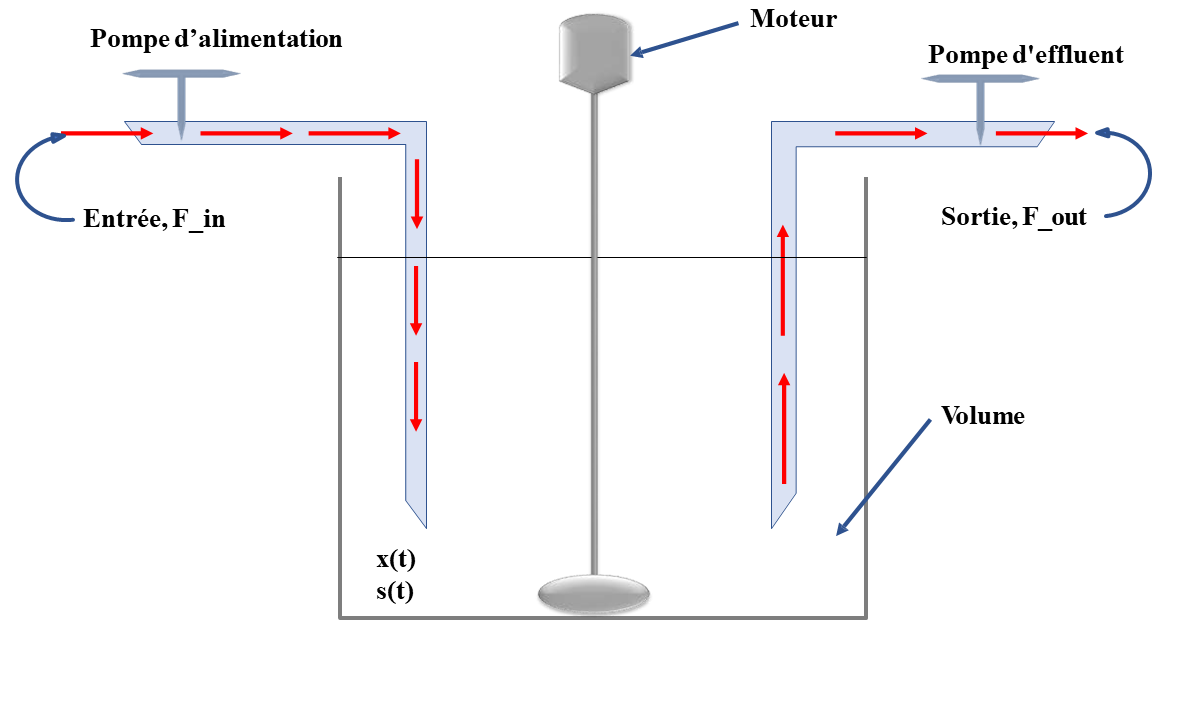
\includegraphics[width=1.05\textwidth]{moha.png} 
    \caption{Bioréacteur, de volume $V$ constant.}
    \label{fig:votre_label}
\end{figure}


{\bf Partie physique}\\
Premièrement, la variation du volume est donnée par 
$$
\frac{d v}{d t}=F_{in} - F_{out} \text {, }
$$
où $F_{in}$ et $F_{out}$ (ou $f_{in}$ et $f_{out}$) flux d'entrée et de sortie (en volume par unité de temps $V/h$).\\
À l'intérieur du chémostat, il n'y a pas d'arrivée d'organismes par le flux. La seule variation de la biomasse des organismes est donc due à la sortie par un flux \( F_{\text{out}} \). Ainsi, on obtient :
$$
\frac{d (v x)}{d t}=-F_{out} x  \text {. }
$$
Pour le substrat, il est nécessaire de prendre en compte le substrat entrant dans le chémostat, à un flux \( F_{\text{in}} \) et avec une concentration \( S_{\text{in}} \), ainsi que la quantité de substrat présente dans la cuve, qui est évacuée par dilution à un flux \( F_{\text{out}} \). Par conséquent, on a :
$$
\frac{d (v s)}{d t}=F_{in} S_{in}-F_{out} s \text {. }
$$
A noter que nous nous concentrerons essentiellement sur le cas où $S_{in}$ reste constante.

{\bf Partie biologique}\\
Les micro-organismes consomment le substrat pour leur croissance. Soit $\mu(s)$ est le taux de croissance ou fonction de croissance spécifique des micro-organismes, qui correspond à la consommation d'une quantité $s$ de substrat. Ainsi, on peut écrire :
$$
\frac{d (v x)}{d t}=\mu(s) (v x).
$$
La quantité de substrat consommée par les micro-organismes diminue à un taux $\sigma(s)$ appelé taux d'absorption.
$$
\frac{d (v s)}{d t}=-\sigma(s) (v x).
$$

En combinant les deux parties, physique et biologique, on obtient le modèle à une espèce de micro-organismes :
\begin{equation}\label{1}
  \left\{\begin{aligned} \frac{d v}{d t} & =F_{\text {in }}-F_{\text {out }}, \\
   \frac{d(s v)}{d t} & =F_{\text {in }} S_{\text {in }}-F_{\text {out }} s-\sigma(s)(v x), \\ 
   \frac{d(x v)}{d t} & =\mu (s)(x v)-F_{\text {out }} x .\end{aligned}\right.
\end{equation}

Le rapport
$$
\gamma(s):=\frac{\mu(s)}{\sigma(s)},
$$
décrit le rendement de conversion du substrat $s$ en biomasse $x$.\\
Il existe trois modes de fonctionnement dans un bioréacteur :\\
1- {\bf Le mode fermé}: ou "batch" en anglais : Les flux d'entrée et de sortie sont nuls. ($F_{\text {in }}=F_{\text {out }}=0$),$ v(0)= V \;\; ,x(0) = X_0$ et $s(0) = S_0$. On assiste à une décroissance exponentielle des micro-organismes.\\
\begin{equation}
\left\{\begin{aligned}
\frac{d s}{d t} & = -\frac{\mu(s)}{\gamma(s)} x, \\
\frac{d x}{d t} & =\mu(s) x  .
\end{aligned}\right.
\end{equation}
2- {\bf Le mode semi-continu } ou "fed-batch" en anglais: Flux de sortie nul ($F_{\text {out }}=0$), $ v(0)= V_0 \;\; ,x(0) = X_0$ et $s(0) = S_0$. C'est le mode de fonctionnement préféré lorsque l'objectif est le contrôle de la population.\\
\begin{equation}
\left\{\begin{aligned}
\frac{d v}{d t} & =F_{\text {in }}, \\
\frac{d s}{d t} & =\frac{F_{\text {in }}}{v} S_{in}-\frac{F_{\text {in }}}{v} s -\frac{\mu(s)}{\gamma(s)} x, \\
\frac{d x}{d t} & =\mu(s) x -\frac{F_{\text {in }}}{v} x .
\end{aligned}\right.
\end{equation}
3- {\bf Le mode continu }: C'est le mode de fonctionnement typique pour le chémostat : le flux de sortie est égal au flux d'entrée ($F_{\text {in }}=F_{\text {out }}\neq 0$), \;$ v(0)= V \;\; ,x(0) = X_0$ et $s(0) = S_0$. Le volume est donc constant dans le réservoir.
\begin{equation}
\left\{\begin{aligned}
\frac{d s}{d t} & =D\left(  S_{in}- s\right) -\frac{\mu(s)}{\gamma(s)} x, \\
\frac{d x}{d t} & =\left( \mu(s)  -D\right) x .
\end{aligned}\right.
\end{equation}
Dans cette partie, on suppose que $\gamma$ est constante, c’est-à-dire que le taux de croissance est proportionnel au taux d’absorption. Cette constante de proportionnalité $\gamma$ est appelée taux de conversion ou rendement de croissance. Le modèle s’écrit sous la forme avec un changement d’unité de $x$ :
\begin{equation}\label{1.1}
\left\{\begin{aligned}
\frac{d s}{d t} & =D \left(S_{in}-s\right) - \mu(s)x, \\
\frac{d x}{d t} & =(\mu(s)-D) x .
\end{aligned}\right.
\end{equation}
Nous nous limiterons à deux hypothèses concernant la fonction $\mu$ :\\
(H1) La fonction $\mu: \mathbb{R}^{+} \rightarrow \mathbb{R}^{+}$ est bornée.\\
(H2) $\mu(0)=0$ et $\mu(s)>0$ pour tout $s>0$.\\
La première hypothèse assure l'existence et l'unicité des solutions de \eqref{1.1}, tandis que la deuxième stipule qu'en l'absence de substrat, il n'y a pas de croissance. L'absence de croissance implique l'absence de consommation du substrat.

Il y a plusieurs catégories de taux de croissance dans la littérature qui vérifient ces hypothèses. Dans le paragraphe suivant, nous en mentionnons quelques-uns. 

\section{Propriétés mathématiques du modèle}
Dans toute cette section, nous supposerons que la fonction \(\mu\) est de classe \(C^1\), positive et nulle en 0. Nous considèrerons qu'elle est strictement croissante, mais nous envisagerons également la possibilité qu'elle soit d'abord strictement croissante puis strictement décroissante.
\subsection{Existence et unicité de la solution positive}
$\blacklozenge$ Dans le mode continu du chémostat, nous avons:
\begin{equation}\label{1.2}
\left\{\begin{aligned}
\frac{ds(t)}{dt} & = D \left(S_{in} - s(t)\right) - \mu(s(t))x(t), \\
\frac{dx(t)}{dt} & = (\mu(s(t)) - D)x (t),\\
s(0)&=s_0, x(0)=x_0.
\end{aligned}\right.
\end{equation}

\begin{théorème}{}{}
Le système \eqref{1.2} admet une solution unique définie sur l'intervalle \(I=[0,+\infty[\). De plus, si les conditions initiales sont positives, c'est-à-dire \(s(0) = s_0\) et \(x(0) = x_0\) avec \(s_0\) et \(x_0\) positives, Alors, la solution \((s(t), x(t))\) reste positive pour tout \(t \geqslant 0\).
\end{théorème} 
\begin{proof}
On pose $X(t)=\begin{pmatrix} 
 s(t) \\ 
 x(t)  
 \end{pmatrix}$ alors \(\dot{X}(t)=f(X(t))\) et
$$
 f : (\mathbb{R}^2_+, \|.\|_{1}) \rightarrow \mathbb{R}^2, \quad f(X) =\left( D \left(S_{in}-s\right) - \mu(s)x ,\;(\mu(s)-D) x \right).
$$
dans ce cas $f$ est lipschitzienne\footnote{ C'est-à-dire $\exists k >0$: pour tout $x,y \in\mathbb{R}^2_+$ $\Rightarrow$ \( \| f(x) - f(y) \| \leq k \| x - y \| \) .}. En effet soient $X, Y$ dans $\mathbb{R}^2_+$:
$$
\begin{aligned}
\|f(X) - f(Y)\|_1 &= |D(s' - s) + \mu(s')x' - \mu(s)x| + |(\mu(s) - D)x - (\mu(s') - D)x'|, \\
&\leq |D||s' - s| + \mu_{\text{max}}|x' - x| + |(\mu_{\text{max}} + D)||x - x'|,\\
&\leq |D||s' - s| + |(2\mu_{\text{max}} + D)||x - x'|,\\
&\leq M (|s' - s|+|x - x'|),\\
&= M \|X-Y\|_1.
\end{aligned}
$$
et $M=D+2\mu_{max}>0$.\\


En conséquence, le théorème d'existence et d'unicité des solutions s'applique (voir Théorème \ref{theorem:existance}). Par conséquent, le système \eqref{1.2} possède une solution unique définie sur l'intervalle \(I=[0,+\infty[\).

Pour la première équation du système, on a 
$$
\begin{aligned}
\frac{d s(t)}{d t} & =D S_{in}-Ds(t)-\mu(s(t))x(t), \\
& \geq -Ds(t)-\mu(s(t))x(t),\\
& \geq -s(t) \left( D+h(s(t))x(t)\right).
\end{aligned}
$$
Avec $h(s)= \frac{\mu_{max}}{s+K}$ ou $h(s)= \frac{m}{K+s+s^2}$.\\
On pose 
$$
 \frac{d z(t)}{d t}=-z(t) \left( D+h(z(t))x(t)\right) \;\;\; z(0)=z_0=s_0,
$$
alors $z(t)=s_0 e^{-\int_0^t\left( D+h(z(\tau))x(\tau)\right)d\tau}$.\\
D'après théorème de comparaison, on a
$$
s(t) \geq s_0 e^{-\int_0^t\left( D+h(z(\tau))x(\tau)\right)d\tau}.
$$
Ainsi, si $s_0 \geq 0$ alors $s(t) \geq 0$ pour tout $t \geq 0$.\\
Pour la deuxième équation du système, on a
$$
x(t)=x_0e^{\int_0^t(\mu(s(v))-D)dv}.
$$ 
Donc, $x$ et positive si et seulement si $x_0$ positive.
\end{proof}
\begin{remarque}{}
$\blacklozenge$ Le segment  
$$
I=\left\lbrace  (s, x): \; s\geqslant 0, \; x \geqslant 0\;\;et\; s+x=S_{in}\right\rbrace,
$$
est positivement invariant et  est un attracteur de toutes les solutions du système \eqref{1.2}. \\
Si on pose $z=s+x$, alors $\frac{d z(t)}{dt}=D(S_{in}-z(t))$
ce qui implique:
$$
z(t)=S_{in}+\left(s(0)+x(0)-S_{in}\right)e^{-D t} \;\; et\;\; \lim\limits_{t\longrightarrow +\infty}z(t)=S_{in}.
$$
$\blacklozenge$ Tous les points d'équilibre $(s^*,x^*)$ du système \eqref{1.2} vérifient $s^*+x^*=S_{in}$.\\
$\blacklozenge$ Les solutions sont bornées. Cela découle immédiatement du fait que $t \rightarrow z(t)$ est bornée
et que $s, \; x$ sont positives.
\end{remarque}
Afin de poursuivre la discussion sur les équilibres, il faut avoir des informations sur la fonction $\mu$.
\subsection{Le taux de croissance de biomasse $\mu$ est strictement croissant.}
Nous supposons que la fonction $\mu$ est de classe $C^1$, avec les hypothèses (H1), (H2), et la condition suivante:\\
(H3) $\mu^{\prime}(s) > 0$ pour tout  $s\geqslant 0$.\\
Cette fonction est appelée fonction de type "{\bf Monod}"(voir figure \ref{Gmonod}). La bornitude rend compte du fait que le microorganisme ne peut absorber qu'une quantité limitée de nutriments.
\begin{figure}[htbp]
  \centering
\begin{tikzpicture}
  \begin{axis}[
    % set axis labels
    xlabel={s},
    ylabel={$\mu(s)$},
    % set axis limits
    xmin=0,
    xmax=10.5,
    ymin=0,
    ymax=5.2,
    xtick=\empty, % effacer les numéros sur l'axe x
    ytick=\empty, % effacer les numéros sur l'axe y
    axis x line=middle, % ajout de la ligne d'axe x
    axis y line=middle, % ajout de la ligne d'axe y
    samples=100, % nombre d'échantillons pour la fonction
  ]
    % set up plot 
    \addplot [domain=-1:10.4, smooth, color=blue] {5*x/(1+x)}; % Plot de la fonction f(x)
    \node [rotate=20] at (axis cs:3.4,4.05) { $s\mapsto \mu(s)$};
   
     \addplot [domain=-1:10.4, smooth, color=red] {4.7}; % Plot de la fonction f(x)
    
    % D = (Sin) label
    \node [rotate=1] at (axis cs:4.3,4.87) { $\mu_{max}$};
   
  \end{axis}
\end{tikzpicture}
  \caption{Fonction de $" Monod "$ .}
  \label{Gmonod}
\end{figure}
Étant $\mu$ croissante et bornée, elle a donc une borne supérieure désignée par: $\mu_{max}=\sup\limits_{s\geq 0}\mu(s)$.\\
La fonction Monod est la fonction: $\mu(s)=\frac{\mu_{max} s}{k+s}$.\\
Elle est évidemment de type {\bf  Monod } et sa borne supérieure est le paramètre $\mu_{max}$. La constante $k$ est appelée constante de  semi-saturation (c'est-à-dire $\mu(k)=\frac{\mu_{max}}{2}$ )
\subsubsection{Les équilibres du système.}
Les équilibres (appelés aussi états stationnaires) s'obtiennent en résolvant le système algébrique:
\begin{equation}
	\left\{\begin{aligned}
		\frac{ds(t)}{d t} & =0 ,\\
		\frac{dx(t)}{d t} & =0.
	\end{aligned}\right.
\end{equation}
Ce qui est équivalent à :
\begin{equation}
\left\{\begin{aligned}
0 & =D \left(S_{in}-s\right) - \mu(s)x, \\
0 & =(\mu(s)-D) x .
\end{aligned}\right.
\end{equation}
La deuxième équation de système implique que $x=0$ ou $\mu(s)=D$. D'où l'on déduit l'équilibre (Sin, 0), appelé équilibre de "{\bf lessivage}". Lorsque $D <\mu_{max}$. On note $\lambda(D)$ la seule solution de l'équation $\mu(s)=D$.
\begin{Proposition}{}\label{Mond}
$\bullet$ Si $\lambda(D)>S_{in}$. le système \eqref{1.2} admet un seul point d'équilibre $E_0=(S_{in}, 0)$ qui est localement stable. Il s'appelle équilibre de lessivage.\\
$\bullet$ Si $\lambda(D) < S_{in}$, le système \eqref{1.2} admet deux points d'équilibre: $E_0 = (S_{in}, 0)$ et $E_1 = (\lambda(D), S_{in} - \lambda(D))$. $E_0$ est un point d'équilibre instable tandis que $E_1$ est un point d'équilibre localement stable. Il s'agit de l'équilibre avec une biomasse positive.
\end{Proposition}
\begin{proof}
Dans le cas où les valeurs propres de la matrice jacobienne sont toutes à partie réelle strictement négative, il y a une stabilité locale.

$\bullet$ La matrice jacobienne du système \eqref{1.2} au voisinage de $E_0$ est égale à :
\[
J(E_0)=\begin{pmatrix}
-D & -\mu(S_{in}) \\
0 & \mu(S_{in})-D
\end{pmatrix}.
\]
Les deux valeurs propres de $J(E_0)$ sont $- D$ et $\mu(S_{in})- D$. Ainsi, l'équilibre $E_0$ est localement stable si et seulement si $\lambda(D)> S_{in}$.

$\bullet$ La matrice jacobienne du système \eqref{1.2} au voisinage de $E_1$ est égale à :
\[
J(E_1)=\begin{pmatrix}
-D -\mu^{\prime}(\lambda(D))(S_{in}-\lambda(D)) & -D \\
\mu^{\prime}(\lambda(D))(S_{in}-\lambda(D)) & 0
\end{pmatrix}.
\]
Les deux valeurs propres de $J(E_1)$ sont $- D$ et $-\mu^{\prime}(\lambda(D))(S_{in}-\lambda(D))$. Alors, si $\lambda(D)<S_{in}$ l'équilibre $E_1$ est localement stable.
\end{proof}
\begin{remarque}{}
 Nous devons ajouter la condition $\lambda(D)< S_{in}$  pour nous assurer de rester dans le cadre positive.
\end{remarque}
Ces résultats sont résumés dans le tableau suivant :

\begin{center}
    \begin{tabular}{|c|c|c|}
        \hline
        \rowcolor{lightgray}
        & $E_0$ & $E_1$ \\
        \hline \hline
        $\lambda(D) > S_{in}$ & localement stable & N'existe pas \\
        \hline
        $\lambda(D) < S_{in}$ & Instable & localement stable \\
        \hline
    \end{tabular}
     \captionof{table}{Les équilibres et leur nature dans le cas où $\mu$ est de type {\bf Monod}.}
\label{tab1}
\end{center}


\subsection{Le taux de croissance de biomasse $\mu$ n'est pas strictement monotone}
Si la fonction \( \mu \) est croissante de manière stricte pour les valeurs petit de \( s \), atteignant son maximum à \( s= s_{m} \), puis décroissant vers $0$ pour les valeurs supérieures à \( s_m \). Nous supposons maintenant que la fonction \( \mu \) est de classe \( C^1 \) et satisfait les hypothèses (H1), (H2) et les hypothèses suivantes  suivantes :\\

(H4) $\mu(0) = 0$ et $\mu^{\prime}(s) > 0$ pour tout  $s<s_m$ et $\mu^{\prime}(s) < 0$ pour tout $s > s_m$ .\\
(H5) $\lim\limits_{s\rightarrow +\infty}\mu(s)=0$.
Cette fonction est de type "{\bf Haldane}".\\
Pour illustrer ce type de fonction, prenons l'exemple de la fonction de Haldane, définie comme suit :
$$
\mu(s)=\frac{m s}{K+s+s^2/l},
$$
$m, K$ et $l$ sont des paramètres strictement positif. Dans cette situation, l'équation \( \mu(s) = D \) peut avoir 0, 1 ou 2 solutions.(voir figure \ref{Ghaldane}).
\begin{figure}[htbp]
  \centering
\begin{tikzpicture}
  \begin{axis}[
    % set axis labels
    xlabel={$s$},
    ylabel={$\mu(s)$},
    % set axis limits
    xmin=0,
    xmax=4.5,
    ymin=0,
    ymax=5.2,
    xtick=\empty, % effacer les numéros sur l'axe x
    ytick=\empty, % effacer les numéros sur l'axe y
    axis x line=middle, % ajout de la ligne d'axe x
    axis y line=middle, % ajout de la ligne d'axe y
    samples=100, % nombre d'échantillons pour la fonction
  ]
    % set up plot 
    \addplot [domain=-1:4.4, smooth, color=blue] {25*x/(1.5 + x + 
    x^2/0.2)}; % Plot de la fonction f(x)
    \node [rotate=-40] at (axis cs:1.6,3.05) {$s\mapsto \mu(s)$};
  
  \end{axis}
\end{tikzpicture}
  \caption{Fonction de $" Haldane "$.}
  \label{Ghaldane}
\end{figure}
\subsubsection{Les équilibres }
De la même manière que dans le cas précédent, les équilibres sont les couples \((s^*, x^*)\) pour lesquels les dérivées sont nulles.

Si $D<s_m$ alors $\exists \lambda(D), \theta(D)$ positive telle que $\mu(\lambda(D))=\mu(\theta(D))=D$. On suppose que  $ \lambda(D)<\theta(D)$
\begin{théorème}{}{}
$\bullet$ Si  $D >s_m$ alors il existe un unique point d'équilibre $E_0=(S_{in} , 0)$ stable.\\
$\bullet$ Si $D<s_m$ alors:
$$
E_0=(S_{in}, 0)\;\;\text{ est un équilibre stable}\; \;\text{si et seulement si} \; \;S_{in}<\lambda(D) \; ou \; S_{in}>\theta(D)
.$$
Pour $S_{in}>\lambda(D)$
$$
E_1=(\lambda(D), S_{in}-\lambda(D))\;\;\text{ est un équilibre stable}.
$$
Et pour $S_{in}>\theta(D)$
$$
E_2=(\theta(D), S_{in}-\theta(D))\; \; \text{ est un équilibre instable}.
$$
\end{théorème}

\begin{proof}
$\bullet$ Pour $D >s_m$ la matrice jacobienne du système \eqref{1.2} en $E_0$ est égale à :
\[
J(E_0)=\begin{pmatrix}
-D & -\mu(S_{in}) \\
0 & \mu(S_{in})-D
\end{pmatrix}.
\]
Les deux valeurs propres de $J(E_0)$ sont $- D$ et $\mu(S_{in})- D$. Ainsi, l'équilibre $E_0$ est localement stable.\\
$\bullet$ Pour $D<s_m$ la matrice jacobienne du système \eqref{1.2} en $E_0$ est égale à :
\[
J(E_0)=\begin{pmatrix}
-D & -\mu(S_{in}) \\
0 & \mu(S_{in})-D
\end{pmatrix}.
\]
Les deux valeurs propres de $J(E_0)$ sont $- D$ et $\mu(S_{in})- D$. Ainsi, l'équilibre $E_0$ est localement stable si et seulement si $S_{in}<\lambda(D)$ ou $S_{in}>\theta(D)$.\\
Si $S_{in}>\lambda(D)$la matrice jacobienne du système \eqref{1.2} en $E_1$ est égale à :
\[
J(E_1)=\begin{pmatrix}
-D-\mu^{\prime}(\lambda(D))(S_{in}-\lambda(D))& & -D \\
& \\
\mu^{\prime}(\lambda(D))(S_{in}-\lambda(D))& & 0
\end{pmatrix}.
\]
Les deux valeurs propres de $J(E_1)$ sont $- D$ et $-\mu^{\prime}(\lambda(D))(S_{in}-\lambda(D))$. L'équilibre $E_1$ est localement stable .\\
Si $S_{in}>\theta(D)$ la matrice jacobienne du système \eqref{1.2} en $E_2$ est égale à :
\[
J(E_2)=\begin{pmatrix}
-D-\mu^{\prime}(\theta(D))(S_{in}-\theta(D))& & -D \\
& \\
\mu^{\prime}(\theta(D))(S_{in}-\theta(D))& & 0
\end{pmatrix}.
\]
Les deux valeurs propres de $J(E_2)$ sont $- D$ et $-\mu^{\prime}(\theta(D))(S_{in}-\theta(D))$. L'équilibre $E_2$ est instable.
\end{proof}
\begin{remarque}{}
 Nous devons ajouter la condition $\lambda(D)< S_{in}$ et $\theta(D)<S_{in}$  pour nous assurer de rester dans le cadre positive.
\end{remarque}
Ces résultats sont résumés dans le tableau suivant :

\begin{center}
    \begin{tabular}{|c|c|c|c|}
        \hline
        \rowcolor{lightgray}
        & $\lambda(D) > S_{in}$ & $\lambda(D) < S_{in} < \theta(D)$ & $\theta(D) < S_{in}$ \\
        \hline \hline
        $E_0$ & Localement stable & Instable & Localement stable \\
        \hline 
       $E_1$ & N'existe pas & Localement stable & Localement stable \\
        \hline
        $E_2$ & N'existe pas & N'existe pas & Instable \\
        \hline
    \end{tabular}
    \captionof{table}{Les équilibres et leur nature dans le cas où $\mu$ est de type {\bf Haldane}.}
\label{tab2}
\end{center}
\begin{Proposition}{ Extinction de la biomasse}\label{rextinction}
Si $\mu_{max}<D$ alors $x(t)$ tend vers zéro exponentiellement. En d’autres termes, la biomasse disparaît.



\end{Proposition}
\begin{proof}
En effet 
$$
\begin{aligned}
	\mu(s(v))-D<\mu_{max}-D &\Leftrightarrow x_0 e^{\int_0^t(\mu(s(v))-D)dv}<x_0e^{\int_0^t(\mu_{max}-D)dv}\\
	&\Leftrightarrow x(t)<x_0e^{(\mu_{max}-D)t}
\end{aligned}
$$
et $\lim\limits_{t \rightarrow \infty} x_0 e^{(\mu_{max} - D)t} = 0$, donc $\lim\limits_{t \rightarrow \infty} x(t) = 0$ ($x$ est positive). Puisque $\lim\limits_{t \rightarrow \infty} (s(t) + x(t)) = S_{in}$, alors $\lim\limits_{t \rightarrow \infty} s(t) = S_{in}$. Ainsi, $(S_{in}, 0)$ est un équilibre globalement stable.
\end{proof}

\section{Diagrammes opératoires}
Dans le cas d'un réacteur de laboratoire, outre les paramètres physico-chimiques tels que le $pH$ ou la température, il existe deux paramètres essentiels qui peuvent être manipulés, à savoir le débit $D$ d'une part, et la concentration en flux $S_{in}$ d'autre part : ce sont ce que nous avons appelé des " entrées " Nous avons vu que le comportement asymptotique du chémostat dépend des relations entre $\lambda(D)$ et $S_{in}$ qui sont résumées dans les tableaux \ref{tab1} et \ref{tab2}.Une manière légèrement plus précise de représenter les choses consiste à localiser les différents résultats possibles dans l’espace des paramètres $(S_{in}, D)$, lorsque $S_{in}$ et $D$ sont fixes, par rapport au graphique de la fonction $S_{in}$ $\mu(S_{in})$. C’est ce qu’on appelle les diagrammes opératoires, une notion définie pour la première fois par le professeur Tewfik SARI.

\subsubsection{$\blacklozenge$ Le cas où la fonction $\mu$ est de type Monod}
  Dans la proposition \ref{Mond}, nous avons observé que la condition requise pour l'existence et la stabilité de l'équilibre $E_1$ est $\lambda(D)<S_{in}$ est équivalent à $D <\mu(S_{in})$. Dans la zone de "lessivage", un seul point d'équilibre stable, $E_0$, est présent, tandis que dans la zone "d'équilibre avec la biomasse", deux points d'équilibre,  $E_0$  instable et $E_1$  stable, sont observés. La courbe $ \mu (S_{in}) =D$ délimite ces deux régions comme illustré sur la figure \ref{diagrame1}.
  \begin{center}
 \begin{tikzpicture}
  \begin{axis}[
    % set axis labels
    xlabel={$S_{in}$},
    ylabel={D},
    % set axis limits
    xmin=0,
    xmax=4.5,
    ymin=0,
    ymax=5.2,
    xtick=\empty, % effacer les numéros sur l'axe x
    ytick=\empty, % effacer les numéros sur l'axe y
    axis x line=middle, % ajout de la ligne d'axe x
    axis y line=middle, % ajout de la ligne d'axe y
    samples=100, % nombre d'échantillons pour la fonction
  ]
    % set up plot 
    \addplot [domain=-1:4.4, smooth, color=blue] {5*x/(1+x)}; % Plot de la fonction f(x)
    
    % D = (Sin) label
    \node [rotate=10] at (axis cs:3.4,4.05) {$D = \mu(S_{in})$};
    
    % Washout label
    \node [rotate=30] at (axis cs:1.2,3.6) {{\bf  Lessivage}};
    
    % Equilibrium with positive biomass label
    \node [rotate=30] at (axis cs:2.3,2) {{\bf  Équilibre avec la biomasse positive}};
  \end{axis}
\end{tikzpicture}
\captionof{figure}[]{Le diagramme opératoires du système ou $\mu$ fonction de "Monod" .}
\label{diagrame1}
\end{center}
  
\subsubsection{$\blacklozenge$ Le cas où la fonction $\mu$ est de type Haldane}
Dans la zone de "lessivage", un seul point d'équilibre stable, $E_0$, est présent, tandis que dans la zone " d'équilibre avec la biomasse", deux points d'équilibre, $E_0$ instable et $E_1$ stable, ainsi que dans la zone de "bi-stabilité", trois points d'équilibre, $E_0$, $E_1$ stable et $E_2$ instable, sont observés. Il est à noter que la courbe d'équation $\mu(S_{in}) = D$ est simplement l'union des graphes des fonctions $S_{in} = \lambda(D)$ et $S_{in} = \theta(D)$, avec $\lambda(D) \in [0, S_m]$ et $\theta(D) \in [S_m, +\infty[$, qui séparent la région "équilibre avec la biomasse" des deux autres régions, ainsi que la droite $D_m = S_{in}$ avec $D_m = \mu(S_m)$, comme illustré sur la figure \ref{diagrame2}.
\begin{center}
  \begin{tikzpicture}
  \begin{axis}[
    % set axis labels
    xlabel={$S_{in}$},
    ylabel={D},
    % set axis limits
    xmin=0,
    xmax=4.5,
    ymin=0,
    ymax=5.2,
    xtick=\empty, % effacer les numéros sur l'axe x
    ytick=\empty, % effacer les numéros sur l'axe y
    axis x line=middle, % ajout de la ligne d'axe x
    axis y line=middle, % ajout de la ligne d'axe y
    samples=100, % nombre d'échantillons pour la fonction
  ]
    % set up plot 
    \addplot [domain=-1:4.4, smooth, color=blue] {25*x/(1.5 + x + 
    x^2/0.2)}; % Plot de la fonction f(x)
    \addplot [domain=0.6:4.4, smooth] {3.87}; % Plot de la fonction f(x)
    % D = (Sin) label
    \node [rotate=-40] at (axis cs:1.6,3.05) {$D = \mu(S_{in})$};
    
    % Washout label
    \node [above] at (axis cs:2,4.1) {{\bf  Lessivage}};
    \node [above] at (axis cs:3,3) {{\bf  Bi-stabilité}};
    
  
    \node [above] at (axis cs:1.4,1) {{\bf  Équilibre avec la}};
    \node [above] at (axis cs:1.44,0.2) {{\bf  biomasse positive}};
  \end{axis}
\end{tikzpicture}
  \captionof{figure}[]{Le diagramme opératoires du système ou $\mu$ fonction de "Haldane" .}
  \label{diagrame2}
\end{center}


\section{Présence de biomasse dans l'alimentation}
Dans de nombreuses applications, le liquide entrant dans le chémostat contient déjà de la biomasse. Par exemple, les bioréacteurs sont utilisés pour traiter les eaux usées, car elles contiennent toutes sortes de bactéries. En présence d'une concentration de $X_{in} > 0$ dans l'écoulement, le modèle \eqref{1.2} devient :
\begin{equation}\label{xin}
	\left\{\begin{aligned}
		\frac{d s(t)}{d t} & =D \left(S_{in}-s(t)\right) - \mu(s(t))x(t), \\
		\frac{d x(t)}{d t} & =D(X_{in}-x(t))+\mu(s(t)) x(t)  ,\\
		s(0)&=s_0   et\; x(0)=x_0.
	\end{aligned}\right.
\end{equation} 
\subsubsection{Propretés générales}
\begin{Proposition}{}
Le système \eqref{xin} admet une solution unique définie sur l'intervalle \(I=[0,+\infty[\). De plus, si les conditions initiales sont positives, c'est-à-dire \(s(0) = s_0\) et \(x(0) = x_0\) avec \(s_0\) et \(x_0\) positives, alors les solutions restent positives pour tout \(t \geq 0\).
\end{Proposition} 
\begin{proof}
On pose $X(t)=\begin{pmatrix} 
 s(t) \\ 
 x(t)  
 \end{pmatrix}$ alors \(\dot{X}(t)=f(X(t))\) et
$$
 f : (\mathbb{R}^2_+, \|.\|_{1}) \rightarrow \mathbb{R}^2, \quad f(X) =\left( D \left(S_{in}-s\right) - \mu(s)x ,\; D \left(X_{in}-x\right) + \mu(s)x \right).
$$
Dans ce cas $f$ est lipschitzienne. En effet soient $X, Y$ dans $\mathbb{R}^2_+$:
$$
\parallel f(X)-f(Y)\parallel_{1}\leq M \parallel X-Y\parallel_{1}
$$
et $M=D+2\mu_{max}$.\\
En conséquence, le théorème d'existence et d'unicité des solutions s'applique (voir Théorème \ref{theorem:existance}). Par conséquent, le système \eqref{xin} possède une solution unique définie sur l'intervalle \(I=[0,+\infty[\).

Pour la premier équation du système \eqref{xin} on a :
$$
\begin{aligned}
\frac{d s(t)}{d t} & =D S_{in}-Ds(t)-\mu(s(t))x(t) \\
& \geq -Ds(t)-\mu(s(t))x(t)\\
& \geq -s(t) \left( D+h(s(t))x(t)\right).
\end{aligned}
$$
Avec $h(s)= \frac{\mu_{max}}{s+K}$ ou $h(s)= \frac{m}{K+s+s^2}$.\\
On pose 
$$
 \frac{d z(t)}{d t}=-z(t) \left( D+h(z(t))x(t)\right) \;\;\; z(0)=z_0=s_0.
$$
Alors $z(t)=s_0 e^{-\int_0^t\left( D+h(z(\tau))x(\tau)\right)d\tau}$.\\
D'après théorème de comparaison \ref{theorem:comparison} on a :
$$
s(t) \geq s_0 e^{-\int_0^t\left( D+h(z(\tau))x(\tau)\right)d\tau}.
$$
Ainsi, si $s_0 \geq 0$ alors  $s(t) \geq 0$ pour tout $t \geq 0$.\\
Pour la deuxième équation du système \eqref{xin} on a :
$$
\begin{aligned}
\frac{d x(t)}{d t} & =D X_{in}-Dx(t)+\mu(s(t))x(t) \\
& \geq -Dx(t)+\mu(s(t))x(t)\\
& \geq -x(t) \left( D-\mu(s(t))\right).
\end{aligned}
$$
On pose 
$$
 \frac{d y(t)}{d t}=-y(t)\left( D-\mu(s(t))\right) \;\;\; y(0)=y_0=x_0.
$$
Alors $y(t)=x_0 e^{-\int_0^t\left( D-\mu(s(\tau))\right)d\tau}$.\\
D'après théorème de comparaison \ref{theorem:comparison} on a :
$$
x(t) \geq x_0 e^{-\int_0^t\left( D-\mu(s(\tau))\right)d\tau}
$$.
Ainsi, si $x_0 \geq 0$ alors $x(t) \geq 0$ pour tout $t \geq 0$.

\end{proof}
$\blacklozenge$ Les solution sont bornées. Cela découle immédiatement du fait que s et x sont positifs et que leur somme s'écrit sous la forme suivante :\\
 $t \rightarrow x(t)+s(t)=X_{in}+S_{in}+(s_0+x_0-X_{in}-S_{in})e^{-t D} $ et que $s$ et $x$ sont positives.
\subsubsection{Les équilibres }
{\bf a) Le cas où $\mu$ de type Monod}.\\
$\blacklozenge$ Les équilibres du système \eqref{xin} sont les solutions du système non linéaire suivant :  
\begin{equation}
	\left\{\begin{aligned}
		0 & =D \left(S_{in}-s\right) - \mu(s)x, \\
		0 & =D(X_{in}-x)+\mu(s) x  .
	\end{aligned}\right.
\end{equation}
La deuxième équation de système implique que $x+s=X_{in}+S_{in}$, et la première équation de système implique: $ D \left(S_{in}-s\right) = \mu(s)x$.\\
Si $x=0$ alors $ (S_{in}-s) =0 $ mais $x+s=X_{in}+S_{in}$, donc $ (S_{in}-s) \neq 0 $.\\
Pour $x > 0$ alors 
$$
\mu(s) =  D \frac{S_{in}-s}{X_{in}+S_{in}-s}.
$$
Si $D > 0$ alors cette équation admet une unique solution $s^*$ telle que $s^* < S_{in}$. On note $(s^*, x^*)$ l'unique point d'équilibre (voir figure \ref{fin1}).
\begin{center}
\begin{tikzpicture}
  \begin{axis}[
    % set axis labels
    xlabel={$s$},
    ylabel={$\mu(s)$},
    % set axis limits
    xmin=0,
    xmax=4.5,
    ymin=-0.8,
    ymax=5.2,
    xtick=\empty, % effacer les numéros sur l'axe x
    ytick=\empty, % effacer les numéros sur l'axe y
    axis x line=middle, % ajout de la ligne d'axe x
    axis y line=middle, % ajout de la ligne d'axe y
    samples=100, % nombre d'échantillons pour la fonction
  ]
    % set up plot 
    \addplot [domain=-1:4.4, smooth, color=blue] {5*x/(1.5 + x)}; 
    \addplot [domain=-1:3.4, smooth, color=uclablue] {5*(3-x)/(4 - x )};
    
    \node [blue,rotate=10] at (axis cs:3,3.8) {$s\mapsto \mu(s)$};
    \node [uclablue,rotate=-20] at (axis cs:1.2,3.7) {$s\mapsto D \frac{(S_{in}-s)}{X_{in}+S_{in}-s}$};
  \node [uclablue,rotate=0] at (axis cs:2.9,-0.5) {$S_{in}$};
  \end{axis}
\end{tikzpicture}
\captionof{figure}[]{Solution de l'équation $\mu(s) =  D \frac{S_{in}-s}{X_{in}+S_{in}-s}$.}
\label{fin1}
\end{center}
\begin{Proposition}{}
	Le point $E=(s^*, x^*)$ est un équilibre localement stable pour le système \eqref{xin}. C'est l'équilibre avec la biomasse positive. 
	
\end{Proposition}
\begin{proof}
	$\bullet$ La matrice jacobienne du système \eqref{xin} au voisinage de $E$ est égale à:
	\[
	J(E)=\begin{pmatrix}
		-D-\mu^{\prime}(s^*) x^* & -\mu(s^*) \\
	    \mu^{\prime}(s^*) x^* & - \frac{D X_{in}}{X_{in}+S_{in}-s^*}
	\end{pmatrix}.
	\]
La trace de $	J(E)$ est:
$$	Tr(J(E))=-D-\mu^{\prime}(s^*) x^* - \frac{D X_{in}}{X_{in}+S_{in}-s^*} < 0.
$$
Le déterminant de $J(E)$ est: 
 $$
 det(J(E))=(D+\mu^{\prime}(s^*) x^*)(\frac{D X_{in}}{X_{in}+S_{in}-s^*})+(\mu^{\prime}(s^*) x^*) (\mu(s^*)) > 0.
 $$
 Les deux valeurs propres de la matrice $J$ sont : $\lambda_1=-D$ et $\lambda_2=-D+\mu(s^*)-\mu^{\prime}(s^*)x^*$. Ainsi, l'équilibre $E$ est localement stable.
	
\end{proof}
\chapter{Préliminaire sur les systèmes différentiels stochastiques}
Dans ce chapitre, nous avons introduit plusieurs définitions, théorèmes et notions fondamentales en calcul stochastique. Ces éléments sont essentiels pour appréhender les concepts qui seront développés dans la suite de ce mémoire.
\section{Processus stochastique et mouvement brownien}
\subsection{Introduction}
Soient ( $\Omega, \mathcal{F}, \mathbb{P}$ ) un espace de probabilité, ( $\mathcal{F}t){t \geq 0} $) une filtration, c'est-à-dire une famille  de sous-tribus croissantes de ( $\mathcal{F}$ ), i.e ($ \mathcal{F}_s \subseteq \mathcal{F}_t $) pour tout ($ t \geq s$ ). Fixons $T \in \R_+$.
\begin{définition}{(Processus stochastique)}
On appelle processus stochastique à valeurs dans un espace $\mathbb{R}^n$ muni d'une tribu $\Bn$\footnote{La tribu de Borel sur $\R^n$.} une famille $X = \lbrace X_t \;: t\in [0, T] \rbrace$ de variables aléatoires définies sur un espace de probabilité $(\Omega,\; \mathcal{F}, \mathbb{P})$ à valeurs dans l'espace mesurable $(\mathbb{R}^n,\mathbb{B}(\mathbb{R}^n))$.
\end{définition}
Il y a plusieurs présentations possibles du mouvement brownien. Par exemple.
\begin{définition}{(Mouvement brownien)}
Un processus $B=(B_t)_{t\geqslant 0}$ à valeurs réelles est appelé mouvement brownien si\\
i) $t\rightarrow B_t$ a une trajectoire continue $\mathbb{P}$-p.s.\\
ii) $B_0=0 \quad \mathbb{P}-p . s $.\\
iii) $\forall\; 0 \leqslant u < s < t$, les variables aléatoire $B_t-B_s$ et $B_s-B_u$ est indépendante.\\
iv) $\forall\; 0 \leqslant s \leqslant t, \quad B_t-B_s \quad \text { est de loi } \mathcal{N}(0, t-s)$ .
\end{définition}
Autrement dit, le processus $B$ commence dès 0. Ses accroissements sont indépendants du passé et sont de loi normale centrée et de variance égale à la longueur de l'intervalle de temps.
\begin{remarque}{}
Lorsque $\left(\mathcal{F}_t\right)_{t \geq 0}$ est la filtration naturelle \footnote{c'est-à-dire $\mathcal{F}_t=\sigma(B_s : s \leq t)$ la tribu engendre par $B$} de $\left(B_t\right)_{t \geq 0}$, on dit que B est un mouvement brownien naturel.
\end{remarque}
On peut généraliser la définition précédente comme suit

\begin{définition}{Mouvement brownien multidimensionnel}
 Un processus $B=\left(\Omega, \mathcal{F},\left(\mathcal{F}_t\right)_{t \geq 0},\left(B_t\right)_{t \geq 0}, \mathbb{P}\right)$ à valeurs dans $\mathbb{R}^d$ est appelé mouvement brownien d-dimensionnel si\\
 i) $t\rightarrow B_t$ a une trajectoire continue $\mathbb{P}$-p.s.\\
ii) $B_0=0 \quad \mathbb{P}-p . s .$\\
iii) $\forall\; 0 \leqslant u < s < t$, le vecteur aléatoire $B_t-B_s$ indépendant à $B_s-B_u$.\\
iv) $\forall\; 0 \leqslant s \leqslant t, B_t-B_s \text { est de loi gaussienne } \mathcal{N}_d\left(0,(t-s) I_d\right),$\\
où $I_d$ est la matrice identité de $\mathbb{R}^d$.
\end{définition}
\begin{définition}{}
Soit $X$ un processus stochastique à valeur dans $\R^n$.\\
i) Le processus $X$ est dit mesurable si l'application $(t, \omega)\longrightarrow X_t(\omega)$ est mesurable de $([0, T]\times \Omega,\mathbb{B}_{[0, T]}\otimes \mathcal{F})$ dans $(\mathbb{R}^n,\mathbb{B}(\mathbb{R}^n))$.\\ 
ii) On dit que $X$ est progressivement mesurable par rapport à une filtration  $(\mathcal{F}_t)_{t\in [0, T]}$ si pour tous $s \in [0, T]$, l'application $(t, \omega)\longrightarrow X_t(\omega)$ est mesurable de 
$([0, s]\times \Omega,\mathbb{B}_{[0, s]}\otimes \mathcal{F}_s)$ dans $(\mathbb{R}^n,\mathbb{B}(\mathbb{R}^n))$.\\ 
\end{définition}
\subsection{Notion de temps d'arrêt d'un processus}
\begin{définition}{}
Soit $(\mathcal{F}_t)_{t \in [0,T[}$ une filtration et $\mathcal{F}_\infty = \sigma (\bigcup\limits_{t \in [0,T[} \mathcal{F}_t)$ sa tribu terminale. Une variable aléatoire $\tau : \Omega \to [0,T[ \cup \{+\infty\}$ est appelée $(\mathcal{F}_t)$-temps d'arrêt si pour tout $t \in [0,T[$, on a $\{\tau \leq t\} \in \mathcal{F}_t$. 
\end{définition}
\begin{définition}{}
Soit \( X \) un processus et \( A \) un sous-ensemble mesurable de l'espace des états \( E \). Les variables aléatoires définies sur \( \Omega \) par
\[
D_A(\omega) = \inf \{t > 0 \;\; :\;X_0\notin A ; X_t(\omega) \in A \},
\]

Pour tout $\omega \in \Omega$ (avec la convention \(\inf \emptyset = +\infty \)). $D_A$ le temps d'entrée dans \( A \).
\end{définition}
\begin{Proposition}{}
On suppose \([0,T[ = [0,a] \) ou \( [0,+\infty[ \) et que \( X \) est un processus continu à valeurs dans un espace métrique \( E \). Si \( A \) est fermé alors \( D_A \) est un temps d'arrêt pour la filtration naturelle de \( X \).
\end{Proposition}
Pour la démonstration, voir \cite{c} page 23.\\
\section{Notion sur le calcul stochastique d'Itô}
\subsection{L'intégrale stochastique et formule d'Itô }
\subsubsection{Intégrale stochastique des processus élémentaires}
Dans l'Analyse du 18\textsuperscript{ème} siècle, l'intégration est vue comme l'opération inverse de la dérivation. Si \( y(t) \) est une fonction définie sur \( [0, a] \) et que sa différentielle est \( dy(t) = f(t)dt \), où \( f \) est une fonction régulière, alors \( y(t) \) peut être récupérée en intégrant les accroissements de \( y \) de \( 0 \) à \( t \), soit \( y(t) - y(0) = \int_{0}^{t} f(s) ds \). Plus généralement, si les accroissements de \( y \) sont de la forme \( dy(t) = f(t)dg(t) \), avec \( g \) à variation bornée, alors \( y(t) - y(0) = \int_{0}^{t} f(s)dg(s) \) (intégrale de Riemann-Stieltjes).

Dans le contexte des processus stochastiques, notamment les mouvements browniens continus \( B_t \), on peut rencontrer des processus \( Y \) dont les accroissements \( dy_t \) sont de la forme \( dy_t = X_t dB_t \), avec \( X_t \) adapté à la filtration \( \mathcal{F}_t \) et régulier. Pour reconstruire \( Y \) en "sommant" ses accroissements, il faut donner un sens à de telles expressions.
\[
\int_0^tX_s(\omega)dB_s(\omega).
\]
Cependant, le mouvement brownien n'est pas à variation bornée, donc cette écriture n'a pas de sens au sens de Riemann-Stieltjes. Des méthodes alternatives, telles que l'intégrale stochastique D'Itô, sont utilisées pour donner un sens à de telles expressions dans le cadre des processus stochastiques.
\begin{définition}{}
On dit qu'un processus $X=\left(X_s\right)_{s \in[0, T]}$ est élémentaire s'il existe une subdivision $0=t_0<..<t_n=T$ de l'intervalle $[0, T]$ et des variables aléatoires réelles $\left(X_i\right), i \in\{0,1, \ldots, n-1\}$, telles que
\begin{equation}\label{prsselmo}
\forall t \in[0, T], \forall \omega \in \Omega, \quad X_t(\omega)=\sum_{i=0}^{n-1} X_i(\omega) \mathbf{1}_{\left[t_i, t_{i+1}[\right.}(t),
\end{equation}
et telles que pour tout $i \in\{0,1, \ldots, n-1\}, X_i$ soit $\mathcal{F}_{t_i}$ mesurable. Autrement dit dans chaque intervalle de temps $\left[t_i, t_{i+1}\left[, X_t(\omega)\right.\right.$ ne dépend pas de t et vaut $X_i(\omega)$.
\end{définition}
On notera alors $\mathcal{E}$ (resp. $\mathcal{E}_n, n>0$ ) l'ensemble de tous les processus élémentaires sur $[0, T]$ (resp. le sous-ensemble des $X \in \mathcal{E}$ tels que les variables aléatoires $X_i$ ont un moment d'ordre n, i.e. $\left.\mathbb{E}\left(\left|X_i\right|^n\right)<+\infty\right)$.
\begin{définition}{}
 On appelle intégrale stochastique (au sens d'Itô) du processus $X \in \mathcal{E}$ donné par \eqref{prsselmo}, la variable aléatoire réelle
$$
\int_0^T X_t d B_t:=\sum_{i=0}^{n-1} X_i\left(B_{t_{i+1}}-B_{t_i}\right)
$$
\end{définition}
Nous définissons la classe des processus qu'on peut intégrer par rapport au mouvement brownien.
\begin{définition}{}
Soit $X=\left(X_t\right)_{t \in[0,T]}$ un processus défini sur l'espace filtré $\left(\Omega, \mathcal{F},\left(\mathcal{F}_t\right)_{t>0}, \mathbb{P}\right)$ du mouvement brownien continu $B$.\\
On dit que $X$ est dans la classe $M^2$ si $X$ est progressivement mesurable et si:
\begin{equation}\label{m2}
\mathbb{E}\left(\int_0^T X_t^2 d t\right)<+\infty,
\end{equation}
où $\int_0^T X_t^2 d t$ est la variable aléatoire. Qui pour tout $\omega \in \Omega$ égale à l'intégrale de Lebesgue $\int_0^T X_t^2(\omega) d t$.\\
\end{définition}
\begin{exemple}{}
Calculons l'intégrale stochastique \(\int_0^1 \sigma \, dB_t\) avec \(x_t = \sigma\) constante. Il est clair que \(x_t \in M^2\). En effet, (\(\mathbb{E}\left(\int_0^1 x_t^2 \, dt\right) = \mathbb{E}\left(\int_0^1 \sigma^2 \, dt\right) = \sigma^2 < +\infty\)). \\
Donc, \(\int_0^1 \sigma \, dB_t = \sigma B_1\).
\end{exemple}
\begin{remarque}{}
On a clairement $\mathcal{E}_2 \subset M^2 $ et $M^2$ (resp. $\mathcal{E}_2$ ) est un espace vectoriel . En fait c'est $M^2$ qui a la structure la plus intéressante car c'est un espace de Hilbert. On constate que tout $X \in M^2$ s'identifie à un élément de $L^2\left([0,T] \times \Omega, \mathcal{B}_{[0,T]} \otimes \mathcal{F}, d t \otimes d \mathbb{P}\right)$ puisque la condition \eqref{m2} s'écrit
$$
\|X\|_{L^2([0,T] \times \Omega, d t \otimes \mathbb{P})}^2 = \mathbb{E}\left(\int_0^T X_t^{2} d t\right) = \int_{[0,T] \times \Omega}\left(X_t(\omega)\right)^2 d t\otimes d \mathbb{P}<+\infty .
$$
\end{remarque}


\begin{Proposition}{}
L'ensemble $\mathcal{P}rog$ de toutes les parties $A \subset[0,T] \times \Omega$ telles que le processus $(t, \omega) \mapsto 1_A(t, \omega)$ est progressivement mesurable, est une sous-tribu de $\mathcal{B}_{[0,T]} \otimes \mathcal{F}$. De plus on a :
\begin{equation}\label{M2}
M^2=L^2([0,T] \times \Omega, \mathcal{P}rog, d t \otimes d \mathbb{P}) .
\end{equation}
\end{Proposition}
\begin{proof}
Il est clair que $A \in \mathcal{P}rog$ si et seulement si pour tout $s \in[0,T], A \cap[a, s] \times \Omega \in \mathcal{B}_{[a, s]} \otimes \mathcal{F}_s$ et on en déduit que $\mathcal{P}rog$ est une tribu. Soit alors $X$ un processus progressivement mesurable. Par définition, pour tout $x \in \mathbb{R}$ et tout $s \in[0,T]$, l'événement \footnote{$[X \leq x] := \{(t,w) : X_t(w) \leq x\}$ } $[X \leq x] \cap[a, s] \times \Omega$ appartient à $\mathcal{B}_{[a, s]} \otimes \mathcal{F}_s$. Ceci signifie que $[X \leq x] \in \mathcal{P}rog$ i.e. $X$ est mesurable par rapport à la tribu $\mathcal{P}rog$ et le résultat \eqref{M2} en découle aussitôt.
\end{proof} 
{\bf Notation }: Pour simplifier l'écriture, on notera $\|X\|_{M^2}:=\|X\|_{L^2([0,T] \times \Omega, d t \otimes \mathbb{P})}$ la norme du processus $X$ de l'espace de Hilbert $M^2$.
\begin{théorème}{}{}
 L'espace $ \mathcal{E}_2 $ des processus élémentaires de carré intégrable est un sous-espace dense de l'espace de Hilbert \( M^2 \), c'est-à-dire que pour tout \( X_t \in M^2 \), il existe une suite \( (X^{(n)}_t)_{n\in \mathbb{N}} \) de processus élémentaires tels que \( X^{(n)}_t \in \mathcal{E}_2 \) pour tout \( n \) et \(\lim\limits_{n \to \infty} \|X^{(n)}_t - X_t\|_{M^2} = 0\).\\
On a alors :
\[
\lim_{n \to \infty} \int_{0}^{T} X^{(n)}_t \, d B_t = \int_{0}^{T} X_t \, d B_t \;\;\;\;\text{dans} \;\;  M^2.
\]
 \end{théorème}
 Pour la démonstration, voir \cite{c} page 122.\\
\begin{corollaire}{}
Si $X$ dans $M^2$ alors
$$
\int_0^T X_t d B_t
$$
est bien définie et on l'appellera l'intégrale stochastique de $X$ sur l'intervalle $[0, T]$.\\ 
$\int_0^T X_t d B_t$ et est une variable aléatoire gaussienne centré de variance 
$$
\mathbb{E}\left((\int_0^T X_t d B_t)^2\right)=\mathbb{E}\left(\int_0^T X_t^2 d t\right)=\int_0^T\mathbb{E}( X_t^2) d t
$$
\end{corollaire}
\begin{exemple}{}
On va calculer l'intégrale stochastique $\int_{0}^{T} B_t \, dB_t$. Notons tout d'abord que \(B \in M^2\). En effet, \(B\) possède des trajectoires continues, donc il est progressivement mesurable et :
$$
\|B_t\|_{M^2} = \frac{T^2}{2}<\infty
$$
\[ \int_{0}^{T} B_t \, dB_t =\frac{B^2_T}{2}-\frac{T}{2} \]
Le terme $\frac{T}{2}$ peut être interprété comme une sorte d'erreur d'Itô.
\end{exemple}
\begin{définition}{(Intégrale de Stratonovitch)}
Soit \(0 = t_0 < t_1 < \cdots < t_N = T\) une partition de \([0,T]\), et soit
\[
e_t = \sum_{k=0}^{N-1} e_{t_k} \mathbf{1}_{[t_{k}, t_{k+1})}(t),
\]
Un processus élémentaire, adaptée à la filtration canonique du mouvement brownien. L'intégrale de Stratonovitch de \(e_t\) est définie par
\[
\int_{0}^{T} e_t \circ dB_t = \sum_{k=0}^{N-1} \frac{e_{t_k} + e_{t_{k+1}}}{2} (B_{t_k} - B_{t_{k+1}}).
\]
L'intégrale de Stratonovitch \(\int_{0}^{T} X_t \circ dB_t\) d'un processus adapté \(X_t \in M^2\) est définie comme la limite de la suite \(\int_{0}^{T} e_t^{(n)} \circ dB_t\) où \(e^{(n)}\) est une suite de processus élémentaire  convergeant vers \(X_t\) dans \(L^2\). 
\end{définition}
\begin{exemple}{}
On va calculer l'intégrale stochastique $\int_{0}^{T} B_t \, dB_t$  selon  Stratonovitch :
\[ \int_{0}^{T} B_t \, dB_t =\frac{B^2_T}{2} \]

\end{exemple}
\begin{remarque}{}
L'intégrale stochastique d'un processus selon Stratonovitch n'est pas une martingale 
en prend par exemple $\int_{0}^{t} B_s \, dB_s =\frac{B^2_t}{2} $
$$
\mathbb{E}[\frac{B^2_t}{2} | \mathcal{F}_s]=\frac{B^2_s}{2} +\frac{t}{2}-\frac{s}{2}\neq \frac{B^2_s}{2}.
$$
Par contre l'intégrale stochastique d'un processus selon Itô est martingale.
\end{remarque}


\subsubsection{Processus d'Itô et formule d'Itô }
\begin{définition}{Processus d'Itô}
Un processus \( X = (X_t)_{t \in [0,T]} \) défini sur \( (\Omega, \mathcal{F}, \mathbb{P}) \) a valeur dans $\R^n$ et adapté à la filtration \( (\mathcal{F}_t)_{t \in [0,T]} \) est appelé processus d'Itô s'il est de la forme
\begin{equation}\label{itoprocessus}
   X_t = X_0 + \int_{0}^{t} f(s) \, ds + \int_{0}^{t} g(s) \, dB_s 
\end{equation}
où $X_0 \in \mathcal{F}_0$ , $f \in L^1$ et $g\in M^2$ sont des processus.
\end{définition}
Cette définition établit les conditions nécessaires pour que le processus d'Itô soit bien défini et ait certaines propriétés de régularité par rapport aux intégrales stochastiques.

On peut aussi écrire l'équation \eqref{itoprocessus} sous la forme :
$$
\mathrm{d} X_t=f(t) \mathrm{d} t+g(t) \mathrm{d} B_t .
$$

Avant d'introduire la formule d'Itô, notons que les différentielles dans une EDS vérifient les règles suivantes 
$$
\begin{aligned}
& \mathrm{d} B_t \mathrm{d} B_t=\mathrm{d} t, \\
& \mathrm{~d} B_t \mathrm{d} t=\mathrm{d} t \mathrm{~d} B_t=0 .
\end{aligned}
$$

Un outil très important pour résoudre et analyser les EDS est la formule d'Itô donnée par le théorème suivant.

\begin{théorème}{(Formule d'Itô)}{ito}
Soit $X_t$ un processus d'Itô. Pour toute fonction $\Phi(t, X_t) \in \mathcal{C}^{1,2}\left(\mathbb{R}_{+} \times \mathbb{R}^n ; \mathbb{R}\right)$ et tout $0 \leqslant t \leqslant T, \Phi(t, X_t)$ est un processus d'Itô et vérifie l'EDS suivante:
\begin{equation}\label{ito1}
\begin{aligned}
d \Phi(t, X_t)&=\frac{\partial\Phi(t, X_t)}{\partial t}d t+\frac{\partial\Phi(t, X_t)}{\partial X} d X_t +\frac{1}{2} \operatorname{tr}\left(g^T(t) \times\frac{\partial^2\Phi(t, X_t)}{\partial X^2}\times g(t)\right)dt
\end{aligned}
\end{equation}
\end{théorème}
Pour la démonstration, voir \cite{c} page 158.\\
avec
$$
\begin{gathered}
 \frac{\partial\Phi(t, X_t)}{\partial x}=\left[\begin{array}{lll}
\frac{\partial \Phi}{\partial x_1} & \cdots & \frac{\partial \Phi}{\partial x_n}
\end{array}\right], \\
\frac{\partial^2\Phi(t, X_t)}{\partial X^2}=\left(\frac{\partial^2 \Phi}{\partial x_i \partial x_j}\right)_{n \times n}=\left[\begin{array}{ccc}
\frac{\partial^2 \Phi}{\partial x_1 \partial x_1} & \cdots & \frac{\partial^2 \Phi}{\partial x_1 \partial x_n} \\
\vdots & \ddots & \vdots \\
\frac{\partial^2 \Phi}{\partial x_n \partial x_1} & \cdots & \frac{\partial^2 \Phi}{\partial x_n \partial x_n}
\end{array}\right] .
\end{gathered}
$$
Si on note 
$$
\Phi_t=\frac{\partial\Phi(t, X_t)}{\partial t},\; \Phi_x=\frac{\partial\Phi(t, X_t)}{\partial x}\;\;et\;\;\Phi_{x x}=\frac{\partial^2\Phi(t, X_t)}{\partial X^2}.
$$ 
et 
$$
\mathcal{L} \Phi(t,X_t)=\Phi_t(t, X_t)+\Phi_x(t, X_t) f(t)+\frac{1}{2} \operatorname{tr}\left(g(t)^T \Phi_{x x}(t, X_t) g(t)\right)
$$
et donc la formule d'Itô \eqref{ito1} se réécrit avec cette dernière notation
$$
\mathrm{d} \Phi(t, X_t)=\mathcal{L} \Phi(t,X_t) \mathrm{d} t+\Phi_x(t, X_t) g(t) \mathrm{d} B_t .
$$
On appelle l'opérateur \( \mathcal{L} \) l'opérateur de générateur.
\subsection{Équation Différentielle Stochastique}
\begin{définition}{}
Soit \( 0 \leq t \leq T \). On appelle Équation Différentielle Stochastique (EDS en abrégé) sur \([0, T]\), avec donnée initiale \( \xi_0 \), toute relation de la forme :
\begin{equation}\label{eds}
\begin{cases} dX_t = f(t,X_t) \, dt +\sum\limits_{i=0}^{d} g_i(t,X_t) \, dB_i(t) \\ X_0 = \xi_0 \end{cases} 
\end{equation}
où \( X \) est un processus d'Itô sur \([0, T]\) (appelé l'inconnue) a valeur dans $\R^n$, \( \xi_0 \) une variable aléatoire donnée, \( \mathcal{F}_0 \)-mesurable, et \( f:[0, T] \times \R^n \rightarrow \R^n \) et \( g_i:[0, T] \times \R^n \rightarrow \R^{n} \) sont deux fonctions mesurables.
\end{définition}
Résoudre l'EDS \eqref{eds} c'est trouver un processus d'Itô \( X \) sur l'intervalle \([0, T]\) tel que :
\[ X_t = \xi_0 +  \int_0^t f(s, X_s) \, ds +\sum\limits_{i=0}^{d}\int_0^t g_i(s, X_s) \, dB_i(s) \quad \text{pour tout } t \in [0, T]. \]

\subsubsection{Un théorème d'existence et d'unicité pour les EDS}
\begin{théorème}{}{existancesto}
Soient \(f : \mathbb{R}^2 \to \mathbb{R}^2\) et \(g_i : \mathbb{R}^2 \to \mathbb{R}^2\) $i=1,...,d$ des fonctions satisfaisant les conditions suivantes :

1. Condition de Lipschitz global : Il existe une constante \(L > 0\) telle que pour tout \(x, y \in \mathbb{R}^2\),
   \[
   \|f(x) - f(y)\| +\sum\limits_{i=0}^{d} \|g_i(x) - g_i(y)\| \leqslant L \|x - y\|.
   \]

2. Condition de croissance linéaire : Il existe une constante \(C > 0\) telle que pour tout \(x \in \mathbb{R}^2\),
   \[
   \|f(x)\| + \sum\limits_{i=0}^{d}\|g_i(x)\| \leqslant C(1 + \|x\|).
   \]

Alors, pour toute condition initiale \(Y_0 \in \mathbb{R}^2\), il existe un temps \(\delta > 0\) et un processus \(Y_t\) unique, continu et adapté à la filtration, qui satisfait l'équation différentielle stochastique presque sûrement :

\[
dY_t = f(Y_t)dt +\sum\limits_{i=0}^{d} g_i(Y_t)dB_i(t), \quad Y_0 = y,
\]

où \(B_i(t)\) $i=1,...,d$ sont des mouvement brownien (processus de Wiener) indépendants.
\end{théorème}
Pour la démonstration, voir \cite{F} page 163.\\
\begin{exemple}{Équation de Black-Scholes}
Considérons l'équation différentielle stochastique (EDS) suivante :

\[ dX_t = X_t \mu \, dt + X_t \sigma \, dB_t \]

où \( \mu \) et \( \sigma \) sont des constantes.

Nous réécrivons l'EDS en termes d'intégrales :

\[ X_t = X_0 + \int_0^t \mu X_s \, ds + \int_0^t \sigma X_s \, dB_s. \]

Pour simplifier, nous faisons une substitution en utilisant \( Y_t = \ln X_t \). En appliquant la formule d'Itô, nous obtenons :

\[ dY_t = \left( \mu - \frac{1}{2} \sigma^2 \right) dt + \sigma \, dB_t. \]

La solution de cette EDS est :

\[ Y_t = Y_0 + \left( \mu - \frac{1}{2} \sigma^2 \right) t + \sigma B_t, \]

où \( Y_0 = \ln X_0 \).

En revenant à la variable d'origine, nous exponentions des deux côtés pour obtenir :

\[ X_t = X_0 \exp \left( \left( \mu - \frac{1}{2} \sigma^2 \right) t + \sigma B_t \right). \]

La solution de l'équation différentielle stochastique

\[ dX_t = X_t \mu \, dt + X_t \sigma \, dB_t \]

est :

\[ X_t = X_0 \exp \left( \left( \mu - \frac{1}{2} \sigma^2 \right) t + \sigma B_t \right). \]
\end{exemple}
\begin{définition}{Temps de Blow-Up \(\tau_e\) }
Soit \(Y_t\) une solution d'une équation différentielle stochastique définie sur un intervalle \([0, T[\). Le temps de blow-up \(\tau_e\) est défini comme :

\[
\tau_e = \sup \left\{ t \in [0, T[ : \sup_{s \in [0, t[} \|Y_s\| < \infty \right\}.
\]

En d'autres termes, \(\tau_e\) est le plus grand temps jusqu'au-quel la solution \(Y_t\) reste finie. Si \(\tau_e < \infty\), cela signifie que la solution \(Y_t\) devient infinie ou "explose" à \(\tau_e\).
\end{définition}
\begin{exemple}{}
Pour valider la définition du temps de blow-up \(\tau_e\), considérons l'équation différentielle stochastique suivante :
\[
dX_t = \frac{1}{1 - t} X_t \, dt + \frac{1}{1 - t} \, dB_t, \quad X_0 = 0,
\]
où \(B_t\) est un mouvement brownien standard.

la solution de l'EDS est :
\[
X_t = \frac{B_t}{1 - t}.
\]
Le mouvement brownien \(B_t\) est presque sûrement fini pour tout \(t\), mais \(\frac{1}{1 - t}\) devient infinie lorsque \(t \to 1\). Par conséquent, \(\frac{B_t}{1 - t}\) devient infinie à ce moment-là.\\
La solution \(X_t\) présente un blow-up en \(t = 1\), car \(\frac{B_t}{1 - t}\) devient infinie à ce moment. Le temps de blow-up \(\tau_e\) pour cette EDS est donc :

\[
\tau_e = 1.
\]
\end{exemple}
\chapter{Modèle du chémostat stochastique }


\section{Première construction du modèle stochastique}
Les systèmes réels, tels que les chémostats, sont fréquemment sujets à des variations et des incertitudes. Ces fluctuations peuvent provenir de diverses sources, telles que des changements environnementaux, des variations des taux de dilution, des erreurs de mesure ou des fluctuations dans la concentration d'entrée de substrat. Le modèle déterministe ne tient pas compte de ces variations et suppose que toutes les variables évoluent de manière parfaitement prévisible.

Pour modéliser ces fluctuations, nous intégrons un terme de bruit stochastique dans le modèle. Ce bruit peut être représenté par un processus de Wiener \(B(t)\), qui modélise des fluctuations aléatoires continues. En particulier, nous introduisons ce bruit dans les deux équations du système, avec des composantes proportionnelles à la croissance des deux variables \(s(t)\) et \(x(t)\) :

\[ + \sigma_1 s(t) \xi_1 \]
où \(\xi_1 dt = dB_1(t)\) et \(\sigma_1\) est un paramètre mesurant l'intensité du bruit.
\[ + \sigma_2 x(t) \xi_2 \]
où \(\xi_2 dt = dB_2(t)\) et \(\sigma_2\) est un paramètre mesurant l'intensité du bruit.\\
Voici comment le système différentiel devient avec les termes stochastiques ajoutés :
\begin{equation}
	\begin{cases}
	\frac{ds(t)}{dt} = \left( D \left(S_{in}-s(t)\right) - \mu(s(t))x(t)\right) + \sigma_1 s(t) \xi_1  \\
	\frac{dx(t)}{dt} = \left((\mu(s(t))-D) x(t)\right)   + \sigma_2 x(t) \xi_2\\
		s_0 = s_0 \\
		x_0 = x_0
	\end{cases}
\end{equation}
L'intégration de ce terme stochastique transforme les équations déterministes en équations différentielles stochastiques. L'ajout de bruit stochastique modifie les équations de la manière suivante :
\begin{equation}\label{DS}
	\begin{cases}
		ds_t = \left( D \left(S_{in}-s_t\right) - \mu(s_t)x_t\right) dt + \sigma_1 s_t dB_1(t) \\
		dx_t = \left((\mu(s_t)-D) x_t\right) dt + \sigma_2 x_t dB_2(t)\\
		s_0 = s_0 \\
		x_0 = x_0
	\end{cases}
\end{equation}
où \(s_0\) et \(x_0\) sont des constantes positives.
\subsection{Existence et unicité de la solution positive}

\begin{théorème}{Existence et Unicité des Solutions}{exemple2}
	Pour tout $(s_0, x_0) \in \mathbb{R}_+^2$, il existe une unique solution $(s_t, x_t)$ de système \eqref{DS} définie pour tout $t \geq 0$ presque sûrement, cette solution reste dans $\mathbb{R}_+^2$ \\ (i.e. $(s_t, x_t) \in \mathbb{R}_+^2 \; \forall t \geq 0 \;\;\mathbb{P}-p.s.$). 
\end{théorème}
\begin{proof}
	Pour simplifier les calculs, nous pouvons écrire le système d'équations différentielles stochastiques sous une forme matricielle compacte:
	\begin{equation}\label{DS1}
		dY_t = f(Y_t)dt + g_1(Y_t)dB_1(t) + g_2(Y_t)dB_2(t)
	\end{equation}
	
	Avec \( Y_t = (s_t, x_t) \)
	$$
	\begin{array}{rcl}
		f:\mathbb{R}^2 &\to& \mathbb{R}^2\\
		Y &\mapsto &f(Y)=\begin{pmatrix}
			D(S_{in}-s) - \mu(s)x \\
			(\mu(s)-D)x
		\end{pmatrix}
	\end{array}
	$$
	$$
	\begin{array}{rcl}
		g_1:\mathbb{R}^2 &\to& \mathbb{R}^2\\
		Y &\mapsto &g_1(Y)=\begin{pmatrix}
			\sigma_1 s \\
			0
		\end{pmatrix}
	\end{array}
	$$
	$$
	\begin{array}{rcl}
		g_2:\mathbb{R}^2 &\to& \mathbb{R}^2\\
		Y &\mapsto &g_2(Y)=\begin{pmatrix}
			0\\
			\sigma_2 x 
		\end{pmatrix}
	\end{array}
	$$
	{\bf i)} Vérifions la premier condition du théorème d'existence \ref{theorem:existancesto} :\\
	On a déjà monter que $f$ est lipschitzienne dans le cas déterministe, donc il existe $k\geqslant 0$ tel que: $\|f(Y)-f(Z)\| \leq k \|Y-Z\|$ pour tout $Y,Z \in \mathbb{R}^2_+$.
	Pour $g_1$ et $g_2$ on a:\\
	Soient $Y=(x,y), \;Z=(a, b) \in \mathbb{R}^2_+$ 
	$$ 
	\begin{aligned}
		\|g_1(Y)-g_1(Z)\|&=|\sigma_1 x -\sigma_1 a|\\
		&=|\sigma_1| | (x -a)|\\
		&\leq |\sigma_1| \|Y-Z\|
	\end{aligned}
	$$
	et $$ 
	\begin{aligned}
		\|g_2(Y)-g_2(Z)\|&=|\sigma_2 y -\sigma_2 b|\\
		&=|\sigma_2| | (y -b)|\\
		&\leq |\sigma_2| \|Y-Z\|
	\end{aligned}
	$$
	Ainsi 
	$$
	\|f(Y)-f(Z)\|+\|g_1(Y)-g_1(Z)\|+\|g_2(Y)-g_2(Z)\|\leq (k+|\sigma_1|+|\sigma_2|) \|Y-Z\| 
	$$
	pour tout $\;Y,Z \in \mathbb{R}^2_+$\\
	{\bf ii)} Pour la deuxième condition du théorème d'existence \ref{theorem:existancesto}, on commence par \( g_1 \) et \( g_2 \). Soit \( Y \in \mathbb{R}^2_+ \), on a \(\|g_1(Y)\| = |\sigma_1 s| \leqslant |\sigma_1|(1 + \|Y\|)\) et \(\|g_2(Y)\| = |\sigma_2 x| \leqslant |\sigma_2|(1 + \|Y\|)\).\\
	pour $f$ on a $\|f(Y)\|=|D(S_{in}-s) - \mu(s)x|+|(\mu(s)-D) x|$
	\begin{align*}
		|D(S_{in}-s) - \mu(s)x| & = |D S_{in}-D s - \mu(s)x| \\
		& \leqslant D S_{in}+|D s + \mu(s)x| \\
		& \leqslant D S_{in}+(D+\mu_{\text{max}})\|Y\| \\
		& = (D S_{in}+D+\mu_{\text{max}})(1+\|Y\|)
	\end{align*}
	\begin{align*}
		|(D - \mu(s))x| & = |(D - \mu(s))|x| \\
		& \leqslant (D + \mu_{max})|x| \\
		& \leqslant (D + \mu_{max})(1+\|Y\|)
	\end{align*}
	donc 
	$\|f(Y)\|\leqslant L(1+\|Y\|)$ et $L=D S_{in}+D+\mu_{\text{max}}$ (en utiliser toujours le fait que \(|s| \)  et \(|x| \) est bornée par \( 1 + \|Y\| \).\\
	La deuxième condition du théorème d'existence \ref{theorem:existancesto} est satisfaite. Alors il existe $\delta>0 $ et un processus $(s_t, x_t)_{t \in [0,\delta[}$ unique, continue et adapté à la filtration, qui satisfait l'équation \eqref{DS1}. Pour prouver que la solution est globale, il suffit de démontrer que le temps de blow-up \(\tau_e\) est infini presque sûrement (p.s.).\\
	{\bf Définition du Temps d'Arrêt}
	Choisissez $n_0 > 0$ assez grand pour que $s_0, x_0 \in [\frac{1}{n_0}, n_0] $. Pour chaque entier \(n \geq n_0\), le temps d'arrêt \(\tau_n\) est défini par :
	\[
	\tau_n = \inf \left\{ t \in [0, \tau_e[ : \min \{s_t, x_t\} \leq \frac{1}{n} \text{ ou } \max \{s_t, x_t\} \geq n \right\}.
	\]
	-\(\tau_n\) est le premier temps où les solutions \(s_t\) ou \(x_t\) deviennent très petites (\(\leq 1/n\)) ou très grandes (\(\geq n\)). Si on peut montrer que \(\tau_n \to \infty\) lorsque \(n \to \infty\), alors cela implique que \(\tau_e = \infty\).\\
	Clairement, \(\tau_n\) est une suite croissante avec \(n\).  En effet, à mesure que \(n\) augmente, les conditions \(\min \{s_t, x_t\} \leq \frac{1}{n}\) et \(\max \{s_t, x_t\} \geq n\) deviennent plus restrictives, donc le temps d'arrêt \(\tau_n\) augmente.
	Soit \(\tau_\infty = \lim\limits_{n \to \infty} \tau_n\). Par définition, \(\tau_\infty \leq \tau_e\).\\
	$\underline{On\; suppose\; que\; \tau_\infty \; est \;fini}$, alors il existe une paire de constantes \(T > 0\) et \(\epsilon \in ]0, 1[\) telles que :
	\[
	\mathbb{P}\left\{\tau_\infty \leq T\right\} > \epsilon.
	\]
	En d'autres termes, il y aurait une probabilité positive que \(\tau_\infty\) soit inférieur ou égal à \(T\), ce qui impliquerait que \(s(t)\) ou \(x(t)\) devient très petit ou très grand en temps fini.
	
	Par conséquent, il existe un entier \(n_1 \geq n_0\) tel que
	\begin{equation}\label{p1}
		\mathbb{P}\left\{\tau_n \leq T\right\}>\varepsilon, \text{ pour tout } n \geq n_1.
	\end{equation}
	
Considérons V une fonction de classe \(C^2\) définie par: 
	$$
	\begin{array}{rcl}
		V:\mathbb{R}_{+} \times \mathbb{R}_{+} &\to& \mathbb{R}_+\\
		(s, x) &\mapsto &V(s, x)=s - A - A \log \frac{s}{A} + (x - 1 - \log x),
	\end{array}
	$$
	où {\bf \(A = \frac{Da}{m}\)}. Évidemment, cette fonction est non-négative pour \(s, x \geq 0\). En effet, les termes \(s - A - A \log \frac{s}{A}\) et \((x - 1 - \log x)\), sont tous deux non-négatifs.
	
	En utilisant la formule d'Itô (voir Théorème \ref{theorem:ito}), nous obtenons
	$$
	\begin{aligned}
		dV(s, x) = & \frac{s-A}{s}\left[\left(D(s_{in}-s) -\mu(s)x \right) dt + \sigma_1(s-A) dB_1(t)\right] + \frac{1}{2} \sigma_1^2 A dt \\
		& + (x-1)\left[\left(\mu(s)  - D\right) dt + \sigma_2 dB_2(t)\right] + \frac{1}{2} \sigma_2^2 dt \\
		:= & \mathcal{L}V(s, x) dt + \sigma_1(s-A) dB_1(t) + \sigma_2(x-1) dB_2(t),
	\end{aligned}
	$$
	où \(\mathcal{L}\) est l'opérateur générant du système \eqref{DS} et
	$$
	\begin{aligned}
		\mathcal{L}V(s, x)&= D(1-\frac{A}{s})(S_{in}-s)-(s-A)h(s)x+(x-1)(\mu(s)-D)+\frac{1}{2}\sigma_1^2 A+\frac{1}{2}\sigma_2^2\\
		&\leqslant DS_{in}+DA-sh(s)x+Ah(s)x+x\mu(s)-Dx-\mu(s)+D+\frac{1}{2}\sigma_1^2 A+\frac{1}{2}\sigma_2^2\\
		&\leqslant DS_{in}+DA+D+Ah(s)x-Dx+\frac{1}{2}\sigma_1^2 A+\frac{1}{2}\sigma_2^2\\
		&\leqslant DS_{in}+DA+D+Ax\frac{m}{a}-Dx+\frac{1}{2}\sigma_1^2 A+\frac{1}{2}\sigma_2^2\\
		&\leqslant DS_{in}+DA+D+\frac{1}{2}\sigma_1^2 A+\frac{1}{2}\sigma_2^2\\
		&\triangleq C^*
	\end{aligned}
	$$
	Avec $\mu(s)=h(s) s$ et $h(s)=\frac{m}{a+s+ks^2}$ ou $h(s)=\frac{m}{a+s}$\\
	où $C^*$ est une constante positive. Donc,
	\[
	\int_0^{\tau_n \wedge T} dV(s_t, x_t)) \leq \int_0^{\tau_n \wedge T} C^* \, dt + \int_0^{\tau_n \wedge T} \sigma_1 (s - A) dB_1(t) + \int_0^{\tau_n \wedge T} \sigma_2 (x - 1) dB_2(t),
	\]
	En prenant l'espérance des deux côtés, cela implique que
	\begin{equation}\label{p2}
		\begin{aligned}
			\mathbb{E}[V(s_{\tau_n \wedge T}, x_{\tau_n \wedge T})]& \leq V(s_0, x_0) + \mathbb{E} \left[\int_0^{\tau_n \wedge T} C^* \, dt \right]\\
			&\leq V(s_0, x_0) + C^* T. 
		\end{aligned}
	\end{equation}
	l'espérance des termes stochastiques est nulle:
	\[
	\mathbb{E}\left[ \int_0^{\tau_n \wedge T} \sigma_1 (s_t - A) dB_1(t) + \int_0^{\tau_n \wedge T}  \sigma_2 (x_t - 1) dB_2(t) \right] = 0
	\]
	Définissons \(\Omega_n = \{\tau_n \leq T\}\) pour tout \(n \geqslant n_1\). Alors, selon \eqref{p1} \(\mathbb{P}(\Omega_n) \geq \varepsilon\). Notez que pour chaque \(\omega \in \Omega_n\), il existe au moins un \(s_{\tau_n}( \omega)\) ou \(x_{\tau_n}( \omega)\) qui atteint soit \(n\) soit \(\frac{1}{n}\), et alors \(V(s_{\tau_n}, x_{\tau_n})\) est plus grand que l'une des deux quantités suivantes :
	\[
	n - 1 - \log n \quad \text{ou} \quad \frac{1}{n} - 1 - \log \frac{1}{n} = \frac{1}{n} - 1 + \log n.
	\]
	Par conséquent,
	\[
	V(s_{\tau_n}, x_{\tau_n}) \geqslant (n - 1 - \log n) \wedge \left(\frac{1}{n} - 1 + \log n\right).
	\]
	Il en découle de \eqref{p1} et \eqref{p2} que
	$$
	\begin{aligned}
		V(s_0, x_0) + C^* T &\geqslant \mathbb{E}\left[\mathbf{1}_{\Omega_n} V(s(\tau_n), x(\tau_n))\right]\\
		&\geqslant \varepsilon \left[(n - 1 - \log n) \wedge \left(\frac{1}{n} - 1 + \log n\right)\right].
	\end{aligned}
	$$
	En laissant \(n \to \infty\) conduit à la contradiction que \(\infty > V(s_0, x_0) + C^* T = \infty\). Ainsi, nous avons \(\tau_\infty = \infty\) presque sûrement (p.s.) absurde.\\
	
	{\bf Montrons la positivité de la solution:} Puisque nous avons
	
	\[
	dx_t = \left((\mu(s_t) - D)x_t\right) dt + \sigma_2 x_t dB_2(t),
	\]
	
	alors d'après la formule d'Itô, nous avons :
	
	\[
	\begin{aligned}
		d(\log(x_t)) &= \frac{dx_t}{x_t} + \frac{1}{2}(\sigma_2 x_t)^2 \frac{-1}{x_t^2} dt \\
		&= \left((\mu(s_t) - D) - \frac{\sigma_2^2}{2}\right) dt + \sigma_2 dB_2(t).
	\end{aligned}
	\]
	
	Alors,
	
	\[
	\log(x_t) - \log(x_0) = \int_0^t \left((\mu(s_r) - D) - \frac{\sigma_2^2}{2}\right) dr + \int_0^t \sigma_2 dB_2(r),
	\]
	
	\[
	\Rightarrow \;\; x_t = x_0 e^{\int_0^t (\mu(S_r) - D) dr - \frac{\sigma_2^2}{2} t + \sigma_2 B_2(t)}.
	\]
	
	Donc, si \(x_0\) est positive, le processus \((x_t)_{t\geqslant0 }\) reste positive.\\
	pour $s$ on a :
	\[
	\begin{aligned}
		ds_t &= \left( D \left(S_{in}-s_t\right) - \mu(s_t)x_t\right) dt + \sigma_1 s_t dB_1(t)\\
		&=\left( D S_{in}-D s_t - \mu(s_t)x_t\right) dt + \sigma_1 s_t dB_1(t)\\
		&\geqslant - \left( D s_t + \mu(s_t)x_t\right) dt + \sigma_1 s_t dB_1(t)\\
		&\geqslant s_t\lbrace -( D + h(s_t)x_t) dt + \sigma_1 dB_1(t)\rbrace
	\end{aligned}
	\]
	soit $z_t$ un processus qui vérifie :
	$$
	dz_t=z_t\lbrace -( D + h(z_t)x_t) dt + \sigma_1 dB_1(t)\rbrace
	$$
	Avec $z_0=s_0$. Alors d'après la formule d'Itô, nous avons :
	
	\[
	\begin{aligned}
		d(\log(z_t)) &= \frac{dz_t}{z_t} - \frac{1}{2}(\sigma_1)^2 dt\\
		&=-\left( D+h(z_t)+\frac{1}{2}(\sigma_1)^2\right) d t +\sigma_1dB_1(t)
	\end{aligned}
	\]
	Alors,
	\[
	\log(z_t) - \log(z_0) = -\int_0^t \left( D+h(z_t)+\frac{1}{2}\sigma_1^2\right)dr + \int_0^t  +\sigma_1dB_1(r),
	\]
	
	\[
	\Rightarrow \;\; z_t = z_0 e^{-\int_0^t (D+h(z_t)) dr-\frac{1}{2}\sigma_1^2t  + \sigma_1 B_1(t)}.
	\]
	D'après le théorème de comparaison pour les processus \cite{art2}, nous avons \(s_t \geqslant z_t\) p.s. pour tout \(t \geq 0\). De plus, \(z_t\) est positive si et seulement si \(s_0\) est positive. Ainsi, \(s_t\) est positive.
	
\end{proof}
\subsection{Extinction de la biomasse}
Dans cette section, nous discutons des conditions qui prédisent l'échec de la culture continue des micro-organismes, tant dans le cas où le bruit environnemental est ignoré que dans le cas d'intensités importantes de bruits blancs, c'est-à-dire que le bruit peut entraîner l'extinction des micro-organismes dans le réacteur.

\begin{théorème}{}{extinction}
	Soit \( \tilde{D} = D + \frac{1}{2} \sigma_2^2 \). Si : \( \tilde{D} > \mu_{max} \),
	
	alors pour toute valeur initiale donnée \( (s_0, x_0) \in \mathbb{R}_+^2 \), la solution \( (s_t, x_t) \) du système \eqref{DS} satisfait
	
	\[ \limsup_{t \to \infty} \frac{1}{t} \log(x_t) < 0 \text{ p.s.}, \]
	
	ce qui signifie que \( x_t \) tend à zéro exponentiellement presque sûrement. En d'autres termes, les micro-organismes disparaissent avec une probabilité égale à un.
\end{théorème}
\begin{remarque}{}
	Notons que $\mu_{max}=\sup\limits_{s\geqslant 0}\mu(s)$ et $\mu(s)=\frac{m s}{a+s}$ ou $\mu(s)=\frac{m s}{a+s+Ks^2}$.
	
\end{remarque}
\begin{proof}
	
	Par la formule d'Itô, nous avons
	
	\[ \log x_t = \log x_0 + \int_0^t \left[ \mu(s_r) - D - \frac{1}{2} \sigma_2^2 \right] dr + \sigma_2 B_2(t), \]
	
	ce qui implique que
	
	\[ \limsup_{t \to \infty} \frac{1}{t} \log(x_t) = \limsup_{t \to \infty} \frac{1}{t} \int_0^t \left[ \mu(s_r) - D - \frac{1}{2} \sigma_2^2  \right] dr \text{ p.s.} \]
	

	
	$$
	\begin{aligned}
		\limsup_{t \to \infty} \frac{1}{t} \log(x_t) &= \limsup_{t \to \infty} \frac{1}{t} \int_0^t \left[ \mu(s_r) - D - \frac{1}{2} \sigma_2^2  \right] dr \text{ p.s.} \\
		&\leqslant  \limsup_{t \to \infty} \frac{1}{t} \int_0^t \left[\mu_{max}-\tilde{D}   \right] dr \text{ p.s.}
	\end{aligned}
	$$
	
	et $\mu_{max}-\tilde{D}<0$ donc :
	
	$$
	\begin{aligned}
		\limsup_{t \to \infty} \frac{1}{t} \log(x_t) & \leqslant  \limsup_{t \to \infty} \frac{1}{t} \int_0^t \left[\mu_{max}-\tilde{D}   \right] dr \text{ p.s.}\\
		&= \mu_{max}-\tilde{D} \text{ p.s.}\\
		&< 0 \text{ p.s.}
	\end{aligned}
	$$
	
	Ainsi, nous concluons que
	
	\[ \limsup_{t \to \infty} \frac{1}{t} \log(x_t) < 0,\;\text{p.s.} \]
	
	La preuve est complète.
	
\end{proof}
\begin{remarque}{}
	Nous nous référons à la condition du théorème \ref{theorem:extinction}, qui nous indique que les espèces de micro-organismes peuvent disparaître lorsque le taux de dilution \( D \) et l'intensité de bruit blanc ($\sigma_2$) ne sont pas importants. Cependant, si l'intensité du bruit blanc est suffisamment grande pour que la condition du théorème \ref{theorem:extinction}  soit remplie, alors la population de micro-organismes s'éteindra également, ce qui n'arrive jamais dans le système déterministe \eqref{1.2} sans perturbations environnementales. De plus, si le taux de dilution \( D \) est suffisamment grand pour entraîner l'extinction des espèces dans le chémostat déterministe alors que le bruit n'est pas important, les espèces de micro-organismes dans le chémostat stochastique \eqref{DS} disparaîtront également.
	
	Du théorème \ref{theorem:extinction}, sous la condition du théorème \ref{theorem:extinction}, nous obtenons qu'il existe une constante \( \lambda > 0 \) telle que
	
	\[ \limsup_{t \to \infty} \frac{1}{t} \log(x_t) \leq -\lambda. \]
	
	C'est-à-dire, pour une constante arbitrairement petite \( 0 < \epsilon < \min\left(\frac{1}{2}, \frac{\lambda}{2}\right) \), il existe une constante positive \( T_1 = T_1(\omega) \) et un ensemble \( \Omega_\epsilon \) tel que \( \mathbb{P}(\Omega_\epsilon) \geq 1 - \epsilon \) et \( \log(x_t) \leq -\frac{\lambda}{2} t \) pour \( t \geq T_1, \omega \in \Omega_\epsilon \). Alors \( x_t \leq e^{-\frac{\lambda t}{2}} \). Ainsi
	
	\[ \limsup_{t \to \infty}x_t \leq 0, \text{ p.s.}, \]
	
	ce qui, avec la propriété positive de la solution du système \eqref{DS}, implique que
	
	\[ \lim_{t \to \infty} x_t = 0, \text{ p.s.} \]
	
	Ainsi, les espèces de micro-organismes \( x \) s'éteindront exponentiellement presque sûrement. En d'autres termes, la population de micro-organismes disparaîtra à un taux exponentiel avec une probabilité de un.
\end{remarque}
\subsection{Distribution stationnaire et ergodicité}
Supposons que \(X_t\) soit un processus de Markov à temps homogène régulier dans \(\mathbb{R}^n\) décrit par l'équation différentielle stochastique
\begin{equation}\label{pp}
	dX_t = b(X_t) \, dt + \sum_{i=1}^{m} g_i(X_t) \, dB_i(t),
\end{equation}

où les mouvements browniens \(B_i(t), i = 1, \ldots, m\), sont indépendants. La matrice de diffusion est définie par

\[\Lambda(X) = \left( \lambda_{i,j}(X)\right)_{1\leqslant i,j \leqslant n}\;\; \lambda_{i,j}(X) = \sum_{r=1}^{m} g_r^i(X) g_r^j(X)^.\]

Définissons l'opérateur différentiel \(\mathcal{L}\) associé à l'équation \eqref{pp} par

\[\mathcal{L} f(X) = \sum_{i=1}^{n} b_k(X) \frac{\partial f(X)}{\partial X_i} + \frac{1}{2} \sum_{i,j=1}^{n} \Lambda_{i,j}(X) \frac{\partial^2 f(X)}{\partial X_i \partial X_j}.\]
pour tout $f$ de classe $C^2(\mathbb{R}^n;\mathbb{R})$
\begin{définition}{1}
Un processus stochastique ergodique est un processus aléatoire pour lequel les moyennes temporelles le long d'une trajectoire donnée convergent presque sûrement vers les moyennes d'ensemble. Formellement, si \( X_t \) est un processus stochastique ergodique, alors pour toute fonction intégrable \( f \):

\[P\left\{ \lim_{T \to \infty} \frac{1}{T} \int_0^T f(X_t) \, dt = \int_{\mathbb{R}^n} f(x) \, \mu(dx) \right\} = 1,\]
où \( \mathbb{E}[f(X)] \) représente l'espérance mathématique de \( f(X) \).
\end{définition}
\begin{lemme}{ (Rafail Khasminskii, 2011)}\label{rafail}
	Supposons qu'il existe un domaine borné \(U \subset \mathbb{R}^n\) avec une frontière régulière \(\Gamma\), ayant les propriétés suivantes :\\
	- (H6) Dans le domaine \(U\) et un voisinage de celui-ci, la plus petite valeur propre de la matrice de diffusion \(\Lambda(X)\) est éloignée de zéro.\\
	- (H7) Si \(x \in \mathbb{R}^n \setminus U\), le temps moyen \(\tau\) pour que les chemins partant de \(x\) atteignent l'ensemble \(U\) est fini, et \(\sup\limits_{x \in D} \mathbb{E}_x[\tau] < \infty\)  \footnote{$\mathbb{E}_x $ L'espérance du temps \(\tau\) pour que \(X_0 = x\).} pour tout sous-ensemble compact \(D \subset \mathbb{R}^n\).\\
	Alors, le processus de Markov \((X_t)_{t\geqslant 0}\) a une distribution stationnaire \(\mu(\cdot)\). De plus, soit \(f(.)\) une fonction intégrable par rapport à la mesure \(\mu\). Alors la probabilité
	
	\[P\left\{ \lim_{T \to \infty} \frac{1}{T} \int_0^T f(X_t) \, dt = \int_{\mathbb{R}^n} f(x) \, \mu(dx) \right\} = 1,\]
	pour tout \(x \in \mathbb{R}^n\).
\end{lemme}
\begin{remarque}{}\label{rafailr}
	La preuve est donnée dans \cite{rafail}. Pour montrer l'existence de la distribution stationnaire \(\mu(\cdot)\) du système \eqref{DS}, il nous suffit de prendre \(\mathbb{R}_+^2\) comme l'espace entier. Pour valider {\bf(H6)}, nous devons prouver que pour tout domaine borné \(D \subset \mathbb{R}_+^2\), il existe un nombre positive \(M_0\) tel que \(\sum\limits_{i,j=1}^{2} \Lambda_{i,j}(X) \xi_i \xi_j \geq M_0 |\xi|^2\) pour tout \(x \in D\). Pour valider {\bf (H7)}, il est suffisant de montrer qu'il existe un voisinage \( U \) et une fonction \( C^2 \) non négative \( V(s, x) \) telle que, pour tout \( x \in \mathbb{R}_+^2 \setminus U \), \(\mathcal{L} V(s, x)\) soit négatif.
	
	En d'autres termes, hors du voisinage \( U \), le générateur infinitésimal de la fonction de Lyapunov est strictement négatif, ce qui implique que la fonction \( V \) décroît, indiquant la stabilité du système loin de \( U \).
\end{remarque}
\begin{définition}{(Régularité, Récurrence)}Un processus de Markov \(X_t\) est dit régulier, si pour tout \(0 \leqslant T < \infty\),
	
	\[P\left( \sup\limits_{0 \leq t \leq T} |X_t| = \infty \right) = 0.\]
	
	Un processus régulier \(X_t\) décrit par \eqref{pp} avec une matrice de diffusion non singulière (c'est-à-dire, la plus petite valeur propre de \(\Lambda(X)\) est éloignée de zéro dans chaque domaine borné de \(\mathbb{R}^n\)) est dit récurrent s'il existe un domaine borné \(U\) tel que pour tout \(x \in \mathbb{R}^n \setminus U\),
	
	\[P\{\tau_x < \infty\} = 1,\]
	
	où \(\tau_x = \inf \{ t > 0 : X_0 = x, \, X_t \in U \}\) est le temps d'atteinte de \(U\) pour \(X_t\).
\end{définition}
\begin{remarque}{}
	Soit \(X_t\) un processus de Markov homogène temporel régulier dans \(\mathbb{R}^n\). Si \(X_t\) est récurrent par rapport à un domaine borné \(U\), alors il est récurrent par rapport à tout domaine non vide dans \(\mathbb{R}^n\). Comme l'existence de la solution positive pour le modèle \eqref{DS} a été obtenue par le théorème \ref{theorem:exemple2}, il nous suffit de prendre \(\mathbb{R}_+^2\) comme espace entier.
\end{remarque} 
Avant de prouver l'ergodicité, nous définissons les notations :

\[f_{max} = \sup_{t \in [0, \infty)} f(t), \quad f_{min} = \inf_{t \in [0, \infty)} f(t).\]

Définissons une fonction continue \(G : \mathbb{R}_+ \to \mathbb{R}\) par:
$$
\begin{aligned}
	G(s)&=-(D-\sigma_1 \tilde{D} K )(s-S_{in})^2 +\sigma_1(\tilde{D}-m+2\tilde{D} K S_{in})(s-S_{in})\\
	&-\sigma_1(mS_{in}-\tilde{D}(a+S_{in}+KS_{in}^2))
\end{aligned}
$$
et $\tilde{D} = D + \frac{1}{2} \sigma_2^2$
\begin{théorème}{}{}
	Si $\sigma_1$ et $\sigma_2$ satisfont:
	\begin{equation}\label{1}
		\sigma_1 < G_0, \;\; \sigma_1^2 < \frac{-2C}{S_{in}} \wedge D,
	\end{equation}
	\begin{equation}\label{2}
		\tilde{D} <\frac{mS_{in}}{a+S_{in}+KS_{in}^2}, \;\; \sigma_2^2 < 2D,
	\end{equation}
	où \(C = \sup\limits_{s \in (0, \infty)} \frac{G(s)}{a + s +Ks^2}< 0\),  $G_0=\frac{D}{\tilde{D} K} \wedge \frac{4D[mS_{in}-\tilde{D}(a+S_{in}+KS_{in}^2)]}{(\tilde{D}-m+2K\tilde{D}S_{in})^2+4K\tilde{D}[mS_{in}-\tilde{D}(a+S_{in}+KS_{in}^2)]}$, alors pour toute valeur initiale \((s_0, x_0) \in \mathbb{R}_+^2\), il existe une distribution stationnaire \(\mu(\cdot)\) pour le système \eqref{DS} et le système est ergodique.
\end{théorème}
\begin{proof}
	Pour simplifier, notons \( s \) et \( x \) respectivement pour \( s_t \) et \( x_t \). Nous allons vérifier que les conditions {\bf (H6) }et {\bf (H7)} sont remplies sous les conditions \eqref{1},\eqref{2} conformément au Lemme \ref{rafail} concernant l'existence de la distribution stationnaire. Le système \eqref{DS} peut être écrit comme suit :
	$$
	\begin{aligned}
		d\binom{s}{x}=\binom{D\left(S_{in}-s\right)-\mu(s) x}{(\mu(s)-D)x} d t & +\binom{\sigma_1 s}{0} d B_1(t) \\
		& +\binom{0}{\sigma_2 x} d B_2(t)
	\end{aligned}
	$$
	donc la matrice de diffusion est
	$$
	\Lambda(s, x)=\left(\begin{array}{ll}
		\sigma_1^2 s^2 & 0 \\
		0 & \sigma_2^2 x^2
	\end{array}\right) .
	$$
	
	Soit \( B \) un domaine borné dans \(\mathbb{R}_{+}^2\), alors il existe une constante positive $$
	M_0=\min \left\{\sigma_1^2 s^2\right., \left.\sigma_2^2 x^2,(s, x) \in \bar{B}\right\} 
	$$
	telle que
	$$
	\sum_{i, j=1}^2 \lambda_{i j}(s, x) \xi_i \xi_j=\sigma_1^2 s^2 \xi_1^2+\sigma_2^2 x^2 \xi_2^2 \geq M_0|\xi|^2, \text { pour tout }(s, x) \in \bar{B}, \xi \in \mathrm{R}^2 .
	$$
	
	Cela implique que la condition {\bf (H6)} est satisfaite.\\
	Ensuite, nous allons construire une fonction \(C^2\) non négative \( V(S, x) \) et un ensemble fermé \( U \in \mathbb{R}_{+}^2 \) tel que
	$$
	\sup _{(s, x) \in \mathbb{R}_{+}^2 \backslash U} \mathcal{L} V(S, x)<-R<0
	$$
	où \( R \) est une constante positive. Cela assure que la condition {\bf (H7)} est satisfaite.
	
	Choisissez une constante positive \( M \) suffisamment grande telle que : \\
	{\bf (A)} \(\Phi_{max} - M \lambda \leq -2\), où \(\lambda = -C - \frac{S_{in}}{2} \sigma_1^2 > 0\) et la fonction \(\Phi(s)\) sera donnée plus tard dans {\bf (B)}. Définissez une fonction \(C^2\) :
	$$
	H(s, x) = M\left[s - S_{in} - S_{in} \log( \frac{s}{S_{in}}) - \sigma_1 \log x\right] + \frac{1}{2D}\left(s - S_{in} +  x \right)^2 - \log s .
	$$
	
	À partir de l'équation aux dérivées partielles de \(H(s, x)\), nous avons
	$$
	\frac{\partial H(s, x)}{\partial s} = \frac{M(s-S_{in})-1}{s} + \frac{1}{D}\left(s - S_{in} +  x \right).
	$$
	$$
	\frac{\partial H(s, x)}{\partial x} = \frac{-M \sigma_1}{x} + \frac{1}{D}\left(s - S_{in} +  x \right).
	$$
	Alors $\exists !(s^*,x^*)$ tel que  $\nabla H(s^*,x^*)=0$\\
	En effet 
	$\frac{\partial H(s, x)}{\partial s}=\frac{\partial H(s, x)}{\partial x}=0$
	
	$$
	\begin{cases}
		\frac{\partial H(s, x)}{\partial s}=0\\
		\frac{\partial H(s, x)}{\partial x}=0
	\end{cases}
	$$
	$$
	\Leftrightarrow \begin{cases}
		\frac{M(s-S_{in})-1}{s}+\frac{s-S_{in}+\frac{\sigma_1 M s}{1-M(s-S_{in})}}{D}=0\\
		x=\frac{\sigma_1 M s}{1-M(s-S_{in})}
	\end{cases}
	$$
	Si on note $h :]0,\infty [\rightarrow \mathbb{R}$ tel que  $h(s)=\frac{M(s-S_{in})-1}{s}+\frac{s-S_{in}+\frac{\sigma_1 M s}{1-M(s-S_{in})}}{D}$  et bijective  donc  $\exists !s^* >0$ tel que $h(s^*)=0$. Ainsi $\exists !(s^*,x^*)$ tel que  $\nabla H(s^*,x^*)=0$\\
	$$
	\nabla^2 H(s, x)=\begin{bmatrix}
		\frac{1}{D}+\frac{1+MS_{in}}{s^2} & \frac{1}{D} \\
		\frac{1}{D} & \frac{1}{D}
	\end{bmatrix}
	$$
	$\nabla^2 H(s, x) $ est définie positive. Les valeurs propres de $\nabla^2 H(s, x) $ est :
	
	\[ \lambda_1 = \frac{1}{2}\left(\frac{2}{D} + \frac{1 + MS_{in}}{s^2}\right) + \frac{1}{2}\sqrt{\frac{4}{D^2} + \frac{(1 + MS_{in})^2}{s^4}} \]
	\[ \lambda_2 = \frac{1}{2}\left(\frac{2}{D} + \frac{1 + MS_{in}}{s^2}\right) - \frac{1}{2}\sqrt{\frac{4}{D^2} + \frac{(1 + MS_{in})^2}{s^4}} \] 
	positive. Alors $ H(s, x) \geqslant  H(s^*,x^*)$.\\
	Ensuite, nous définissons une fonction \(C^2\) non négative \(V(\cdot, \cdot) : \mathbb{R}_{+}^2 \rightarrow \mathbb{R}_{+}\) par
	
	$$
	V(s, x)= M\left[s - S_{in} - S_{in} \log \frac{s}{S_{in}} - \sigma_1 \log x\right] + \frac{1}{2D}\left(s - S_{in} +  x \right)^2 - \log s - H(s^*,x^*).
	$$
	
	Notons\\
	\(V_1(s, x)=s - S_{in} - S_{in} \log( \frac{s}{S_{in}}), V_2(s, x)=V_1(s, x)-\sigma_1 \log x, V_3(s, x)=\frac{1}{2D}\left(s - S_{in} +  x \right)^2\).
	
	Ainsi,
	
	\begin{equation}\label{3}
		\mathcal{L} V(s, x)=M \mathcal{L} V_2+\mathcal{L} V_3+\mathcal{L}(-\log S) .
	\end{equation}
	Par la formule d'Itô en obtient
	$$
	\begin{aligned}
		\mathcal{L} V_1(s, x)= & \frac{s-S_{in}}{s}\left[D\left(s-S_{in}\right)-\frac{m s x}{a+s+K s^2}\right]+\frac{S_{in}}{2} \sigma_1^2 \\
		& \leq-\frac{D\left(s-S_{in}\right)^2}{s}+\frac{m S_{in} x}{a+s+K s^2}+\frac{S_{in}}{2} \sigma_1^2 \\
		& \leq-\frac{D\left(s-S_{in}\right)^2}{s}+\frac{m S_{in}}{a} x+\frac{S_{in}}{2} \sigma_1^2 \\
		& \leq-\frac{D\left(s-S_{in}\right)^2}{a+s+K s^2}+\frac{m S_{in}}{a} x+\frac{S_{in}}{2} \sigma_1^2,
	\end{aligned}
	$$
	et 
	$$
	\begin{aligned}
		\mathcal{L}(-\log x) & =\tilde{D}-\frac{m s}{a+s+K s^2} \\
		& =\frac{\tilde{D} a+\tilde{D} s+\tilde{D} K s^2-m s}{a+s+K s^2} \\
		& =\frac{\tilde{D} K\left(s-S_{in}\right)^2+\left(\tilde{D}-m+2 \tilde{D} K S_{in}\right)\left(s-S_{in}\right)-\left[m S_{in}-\tilde{D}\left(a+S_{in}+K S_{in}^2\right)\right]}{a+s+K s^2} .
	\end{aligned}
	$$
	ainsi
	\footnotesize{
		$$
		\begin{aligned}
			\mathcal{L} V_2(s, x) \leq & \frac{\sigma_1 \tilde{D} K\left(s-S_{in}\right)^2+\sigma_1\left(\tilde{D}-m+2 \tilde{D} K S_{in}\right)\left(s-S_{in}\right)-\sigma_1\left[m S_{in}-\tilde{D}\left(a+S_{in}+K S_{in}^2\right)\right]}{a+s+K s^2} \\
			& -\frac{D\left(s-S_{in}S\right)^2}{a+s+K s^2}+\frac{m S_{in}}{a} x+\frac{S_{in}}{2} \sigma_1^2 \\
			= & \frac{-\left(D-\sigma_1 \tilde{D} K\right)\left(s-S_{in}\right)^2+\sigma_1\left(\tilde{D}-m+2 \tilde{D} K S_{in}\right)\left(s-S_{in}\right)-\sigma_1\left[m S_{in}-\tilde{D}\left(a+S_{in}+K S_{in}^2\right)\right]}{a+s+K s^2} \\
			& +\frac{m S_{in}}{a} x+\frac{S_{in}}{2} \sigma_1^2 \\
			= & \frac{G(s)}{a+s+K s^2}+\frac{m S_{in}}{a } x+\frac{S_{in}}{2} \sigma_1^2 .
		\end{aligned}
		$$
	}
	Il découle de la condition \eqref{1} que le discriminant de la fonction \( G(.) \) est négatif et que \( D-\sigma_1 \tilde{D} K>0 \). Alors, pour tout \( s \in ]0, \infty[ \), la fonction \( G(s) < 0 \). Prenons \( C = \sup\limits_{s \in ]0, \infty[} \frac{G(s)}{a + s + K s^2} < 0 \), et soit \( \lambda = -C - \frac{S_{in}}{2} \sigma_1^2 > 0 \), alors nous obtenons
	\[
	\mathcal{L}V_2(s, x) \leq -\lambda + \frac{mS_{in}}{a} x.
	\]
	De plus, puisque \( s^2 \leq 2(s - S_{in})^2 + 2S_{in}^2 \), nous avons
	\begin{equation}\label{4}
		\begin{aligned}
			\mathcal{L} V_3(s, x)= & -\left(s-S_{in}+ x\right)^2+\frac{\sigma_1^2}{2 D} s^2+\frac{\sigma_2^2}{2 D} x^2 \\
			= & -\left( s-S_{in}\right)^2- x^2-2\left(s-S_{in}\right) x+\frac{\sigma_1^2}{2 D} s^2+\frac{\sigma_2^2}{2 D} x^2 \\
			\leq&-\left(1-\frac{\sigma_1^2}{D}\right)\left(s-S_{in}\right)^2-\left(1-\frac{\sigma_2^2}{2 D}\right) x^2+ 2S_{in} x+\frac{S_{in}^2}{D} \sigma_1^2,
		\end{aligned}
	\end{equation}
	et
	\begin{equation}\label{5}
		\begin{aligned}
			\mathcal{L}(-\log (s))= & -\frac{DS_{in}}{s}+D+ \frac{m x}{a+s+K s^2}+\frac{1}{2} \sigma_1^2 \\
			& \leq-\frac{D S_{in}}{s}+D+\frac{m}{a} x+\frac{1}{2} \sigma_1^2 .
		\end{aligned}
	\end{equation}
	En substituant \eqref{4}, \eqref{5} et \eqref{6} dans \eqref{3},
	$$
	\begin{aligned}
		\mathcal{L} V(s, x) &\leq M\left(-\lambda+\frac{m S_{in}}{a} x\right)-\left(1-\frac{\sigma_1^2}{D}\right)\left(s-S_{in}\right)^2-\left(1-\frac{\sigma_2^2}{2 D}\right) x^2 \\
		& +2 S_{in} x-\frac{D S_{in}}{s}+Q+\frac{m}{a} x+\frac{1}{2} \sigma_1^2+\frac{S_{in}^2}{D} \sigma_1^2 \\
		& =\Phi(s)+\Psi(x) \\
		&
	\end{aligned}
	$$
	où {\bf (B)}
	\begin{equation}\label{6}
		\left\{\begin{array}{l}
			\Phi(s)=-\left(1-\frac{\sigma_1^2}{D}\right)\left(s-S_{in}\right)^2-\frac{D S_{in}}{s}+D+\frac{1}{2} \sigma_1^2+\frac{S_{in}^2}{D} \sigma_1^2 \\
			\Psi(x)=-\left(1-\frac{\sigma_2^2}{2 D}\right) x^2+2 S_{in} x+\frac{m}{a} x+M\left(-\lambda+\frac{m S_{in}}{a} x\right) .
		\end{array}\right.
	\end{equation}
	Compte tenu de \eqref{1} et \eqref{2}, nous observons que
	$$
	\begin{aligned}
		& \Phi(s)+\Psi_{max} \rightarrow-\infty, \text { quand } s \rightarrow+\infty, \\
		& \Phi_{max}+\Psi(x) \rightarrow-\infty, \text { quand } x \rightarrow+\infty, \\
		& \Phi(s)+\Psi_{max} \rightarrow-\infty, \text { quand } s \rightarrow 0^{+} .
	\end{aligned}
	$$
	Les cas ci-dessus conduisent respectivement à \(\mathcal{L} V < -1\). De plus, en examinant la condition (A), nous obtenons
	$$
	\Phi_{max}+\Psi(x) \rightarrow \Phi_{max}-M \lambda \leq-2 \text {, as } x \rightarrow 0^{+} .
	$$
	Prenons \(\varepsilon\) suffisamment petit, et soit \( U = \left[\varepsilon, \frac{1}{\varepsilon}\right] \times \left[\varepsilon, \frac{1}{\varepsilon}\right] \). Par conséquent,
	$$
	\mathcal{L} V(s, x)<-1, \;\;(s, x) \in \mathbb{R}^2_+\setminus U .
	$$
	Selon la Remarque \ref{rafailr}, les conditions du Lemme \ref{rafail} sont satisfaites. Ainsi, le modèle de chémostat stochastique \eqref{DS} a une distribution stationnaire et il est ergodique.
\end{proof}
\begin{remarque}{La bornitude de la solution}
	Puisque le système est stationnaire, la solution est bornée, c'est-à-dire que 
	$$s_t \leqslant M  \quad \text{et} \quad s_t \leqslant M \quad p.s.,$$
	où \( M \) est une constante positive.
\end{remarque}



\chapter{Simulation déterministe et stochastique}
\section{Application numérique du première modèle stochastique}
Le schéma d'Euler-Maruyama est une méthode numérique utilisée pour approcher la solution d'équations différentielles stochastiques (EDS). Cette méthode permet de discrétiser les EDS et de les résoudre par des simulations de chemins aléatoires.

Considérons le système suivant d'équations différentielles stochastiques :

\begin{equation}\label{sigma}
	\begin{cases}
		ds_t = \left( D \left(S_{in} - s_t\right) - \mu(s_t)x_t \right) dt + \sigma_1 s_t dB_1(t) \\
		dx_t = \left( (\mu(s_t) - D) x_t \right) dt + \sigma_2 x_t dB_2(t) \\
		s_0 = S_0 \\
		x_0 = X_0
	\end{cases}
\end{equation}

où :\\
- \(\sigma_1\) et \(\sigma_2\) sont des coefficients de diffusion, indiquant l'intensité des fluctuations stochastiques.\\
- \(B_1(t)\) et \(B_2(t)\) sont des mouvements browniens indépendants.

Pour appliquer le schéma d'Euler-Maruyama, nous discrétisons le temps en intervalles de longueur \(\Delta t\), et nous utilisons les approximations suivantes pour les incréments des mouvements browniens : \(\Delta B_1(i) = B_1(t_{i+1}) - B_1(t_i)\) et \(\Delta B_2(i) = B_2(t_{i+1}) - B_2(t_i)\).

Le schéma d'Euler-Maruyama pour ce système peut alors être écrit comme suit :

\[
\begin{cases}
	s_{i+1} = s_i + \left( D \left(S_{in} - s_i\right) - \mu(s_i)x_i \right) \Delta t + \sigma_1 s_i \Delta B_1(i) \\
	x_{i+1} = x_i + \left( (\mu(s_i) - D) x_i \right) \Delta t + \sigma_2 x_i \Delta B_2(i) \\
\end{cases}
\]

où :\\
- \(s_i\) et \(x_i\) sont les approximations des variables \(s_t\) et \(x_t\) à l'instant \(t_i\).\\
- \(s_{i+1}\) et \(x_{i+1}\) sont les approximations des variables \(s_t\) et \(x_t\) à l'instant \(t_{i+1} = t_i + \Delta t\).\\
- \(\Delta B_1(i)\) et \(\Delta B_2(i)\) sont les incréments du mouvement brownien, qui peuvent être modélisés par des variables aléatoires gaussiennes de moyenne nulle et de variance \(\Delta t\).

Ce schéma permet d'obtenir une approximation numérique de la solution du système d'équations différentielles stochastiques en simulant les trajectoires des variables \(s_t\) et \(x_t\) à des instants de temps discrets.
\begin{exemple}{}
	D’après le théorème \ref{theorem:exemple2}, nous nous attendons à ce que, sous certaines conditions appropriées, le système stochastique \eqref{sigma} admette une solution positive. Choisissons les valeurs initiales \((s_0, x_0) = (2, 2)\) et supposons que les paramètres dans \eqref{sigma} sont donnés par \(m = 2\), \(S_{in} = 3\), \(a = 1\), et \(K = 0.1\).
	
	Dans le théorème \ref{theorem:exemple2}, toutes les conditions sont satisfaites. Nous en concluons donc qu’il existe une solution positive bornée (voir les deux sous-graphique dans la figure \ref{fig:fgure11}). Les simulations numériques dans la figure \ref{fig:fgure11} soutiennent clairement cette conclusion, illustrant que l’écart-type \(\sigma\) maintient les processus \(s_t\) et \(x_t\) en mouvement autour de la solution du modèle de chémostat déterministe correspondant.
	
	
\end{exemple}

\begin{figure}[h]
	\centering
	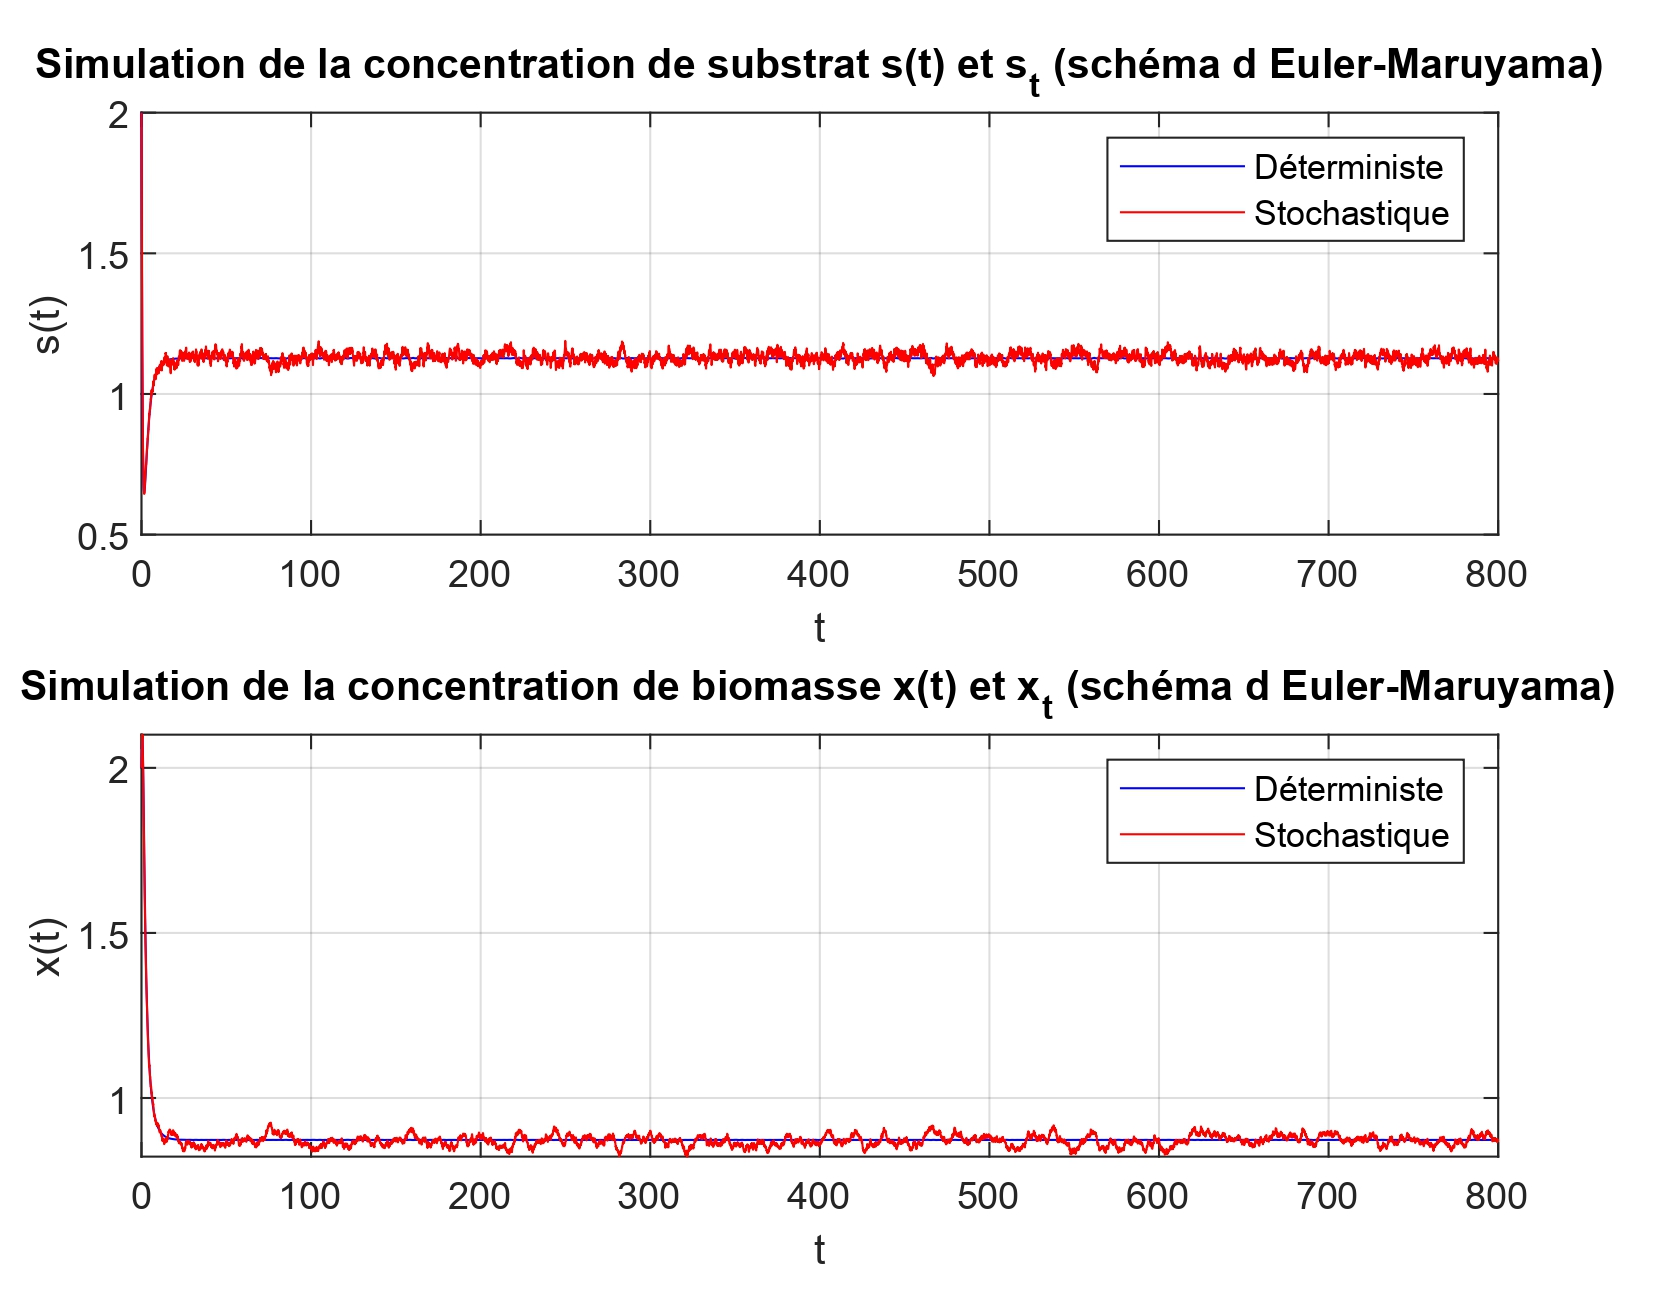
\includegraphics[width=1.05\textwidth]{c1_page-0001.png} 
	\caption{Solutions numériques pour le système \eqref{edssn} et le système déterministe correspondant \eqref{sigma} avec les paramètres principal \( D = 1 \), $\sigma_1=0.02 , \;et \;\; \sigma_2 = 0.01$.}
	\label{fig:fgure11}
\end{figure}
\newpage
\begin{exemple}{}
	On a aussi dans ce cas les conditions du théorème \ref{theorem:exemple2} satisfaites. Pour illustrer davantage l’effet des mouvements browniens \(\sigma_1, \; et\; \sigma_2\) sur le modèle de chémostat stochastique, nous gardons tous les paramètres de l’exemple précédent inchangés mais augmentons les intensités  \(\sigma_1=\sigma_2 = 0.1\). La figure \ref{fig:fgure12} illustre que le bruit blanc maintient toujours les processus \(s_t\) et \(x_t\) se déplaçant autour de la solution du modèle de chémostat déterministe, tandis que les oscillations aléatoires deviennent plus fortes.
	
\end{exemple}
\begin{figure}[h]
	\centering
	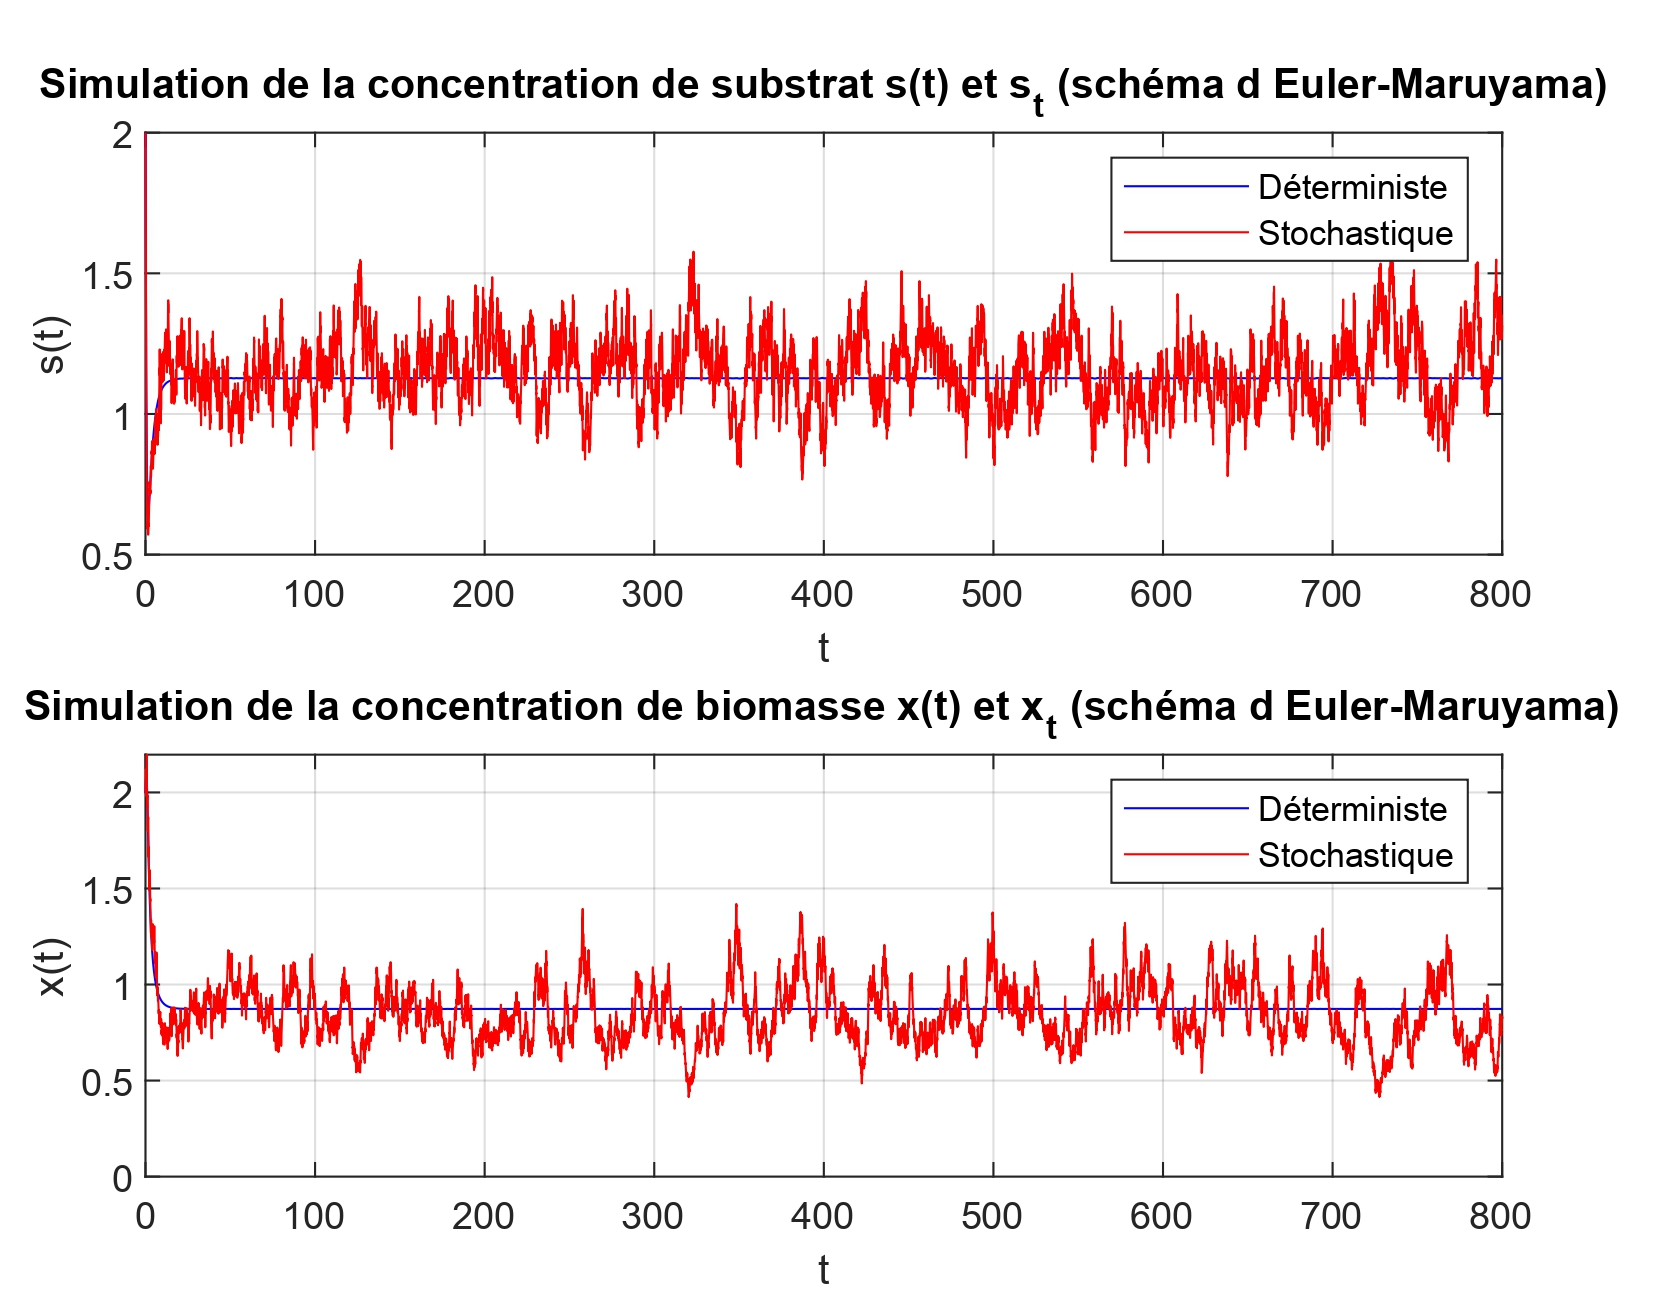
\includegraphics[width=1.05\textwidth]{C2_page-0001.png} 
	\caption{Solutions numériques pour le système \eqref{edssn} et le système déterministe correspondant \eqref{sigma} avec les paramètres principal \( D = 1 \) et $\sigma_1=\sigma_2 = 0.1$.}
	\label{fig:fgure12}
\end{figure}

\newpage
\begin{exemple}{}
	Dans cet exemple, nous avons traité le cas où la dilution est plus grande \( D = 1.5\). Alors, sous les conditions du théorème \ref{theorem:extinction} et de la proposition \ref{rextinction} dans le deuxième chapitre, qui sont satisfaites, nous avons l'extinction exponentielle  de la biomasse dans les deux modèles, déterministe et stochastique. Les simulations numériques dans la figure \ref{fig:fgure13} soutiennent clairement cette conclusion.
	
\end{exemple}
\begin{figure}[h]
	\centering
	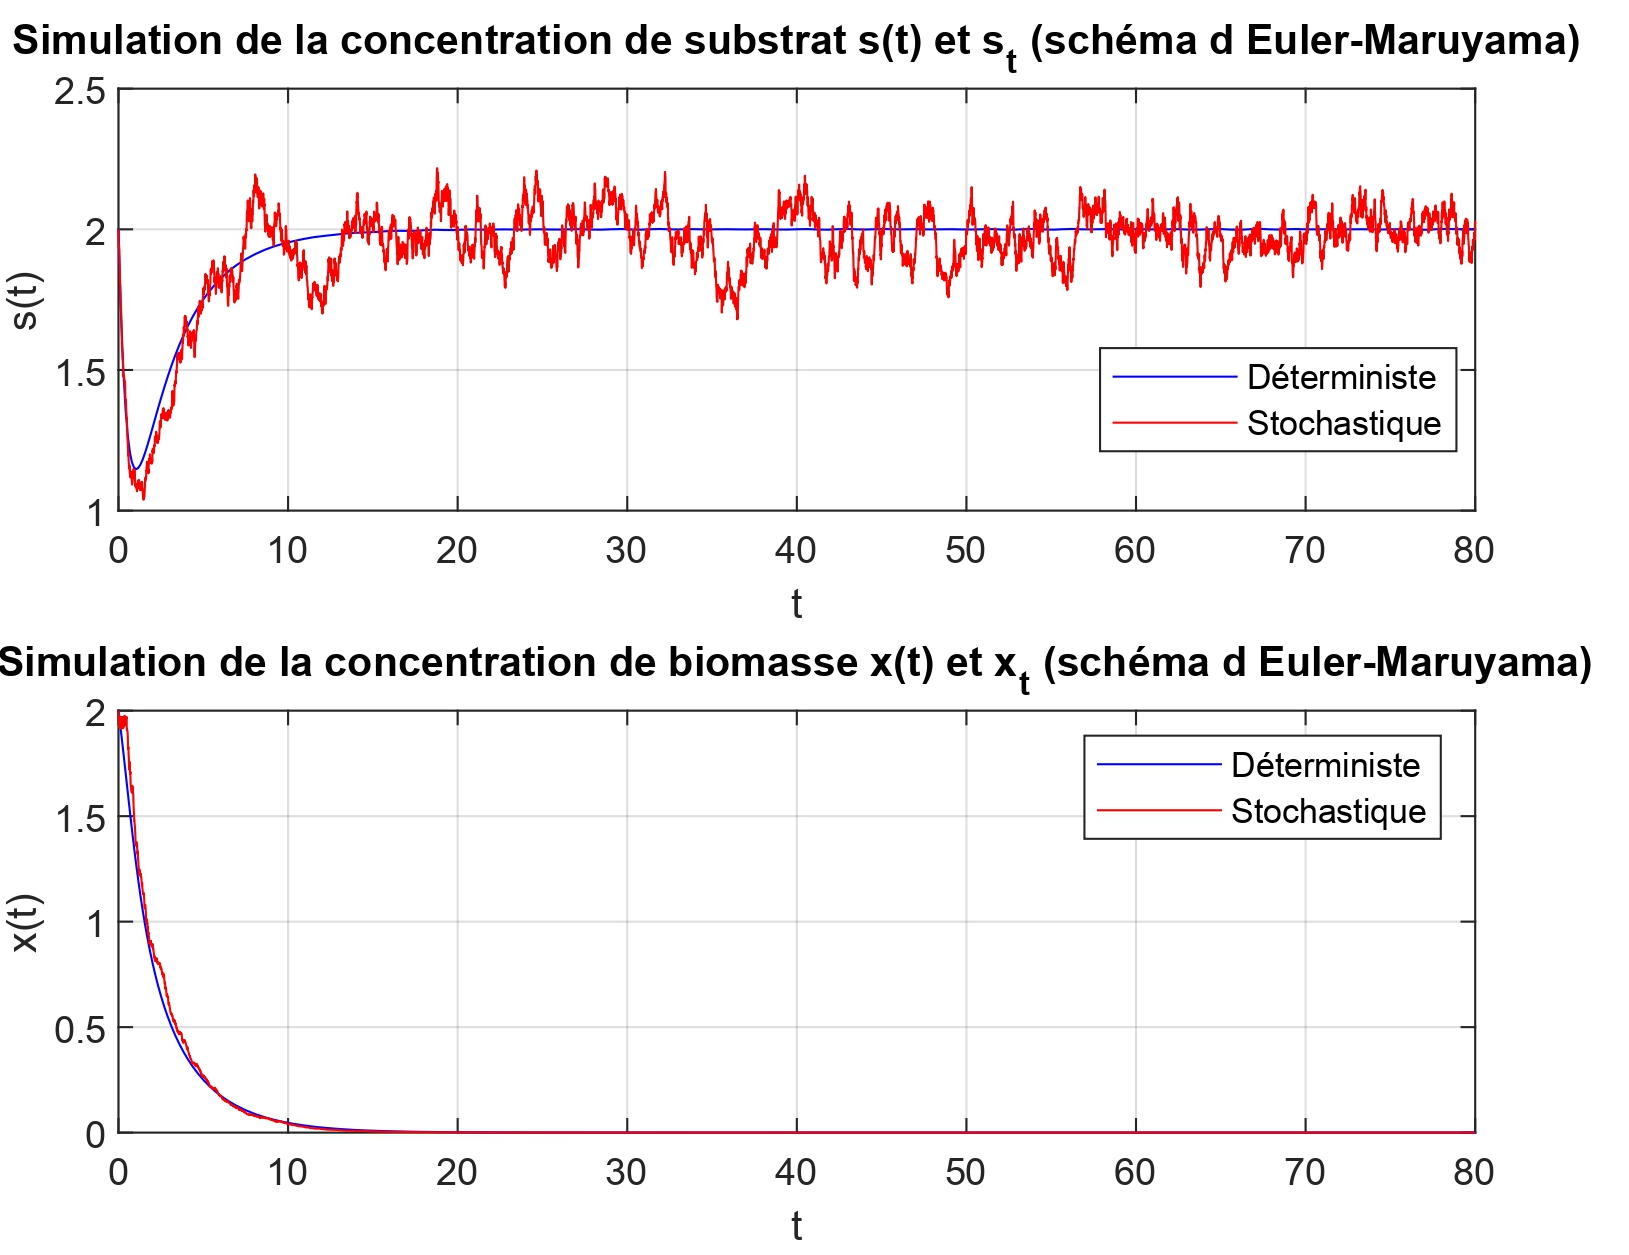
\includegraphics[width=1.05\textwidth]{C3_page-0001.png} 
	\caption{Solutions numériques pour le système \eqref{edssn} et le système déterministe correspondant \eqref{sigma} avec les paramètres principal \( D = 1.5 \), $\sigma_1=0.08 , \;et \;\; \sigma_2 = 0.08$.}
	\label{fig:fgure13}
\end{figure}
\newpage
\begin{exemple}{}
	Maintenant, si nous fixons la dilution \(D = 1\) et les intensités \(\sigma_1 = 0.2 \;\;et\;\; \sigma_2=1.1\), dans ce cas, le système déterministe stable présente toujours une concentration du substrat et une biomasse strictement positives. Par contre, dans le système stochastique, il y a une extinction de la biomasse. Les simulations numériques dans la figure \ref{fig:fgure14} valident ces résultats.
	
\end{exemple}

\begin{figure}[h]
	\centering
	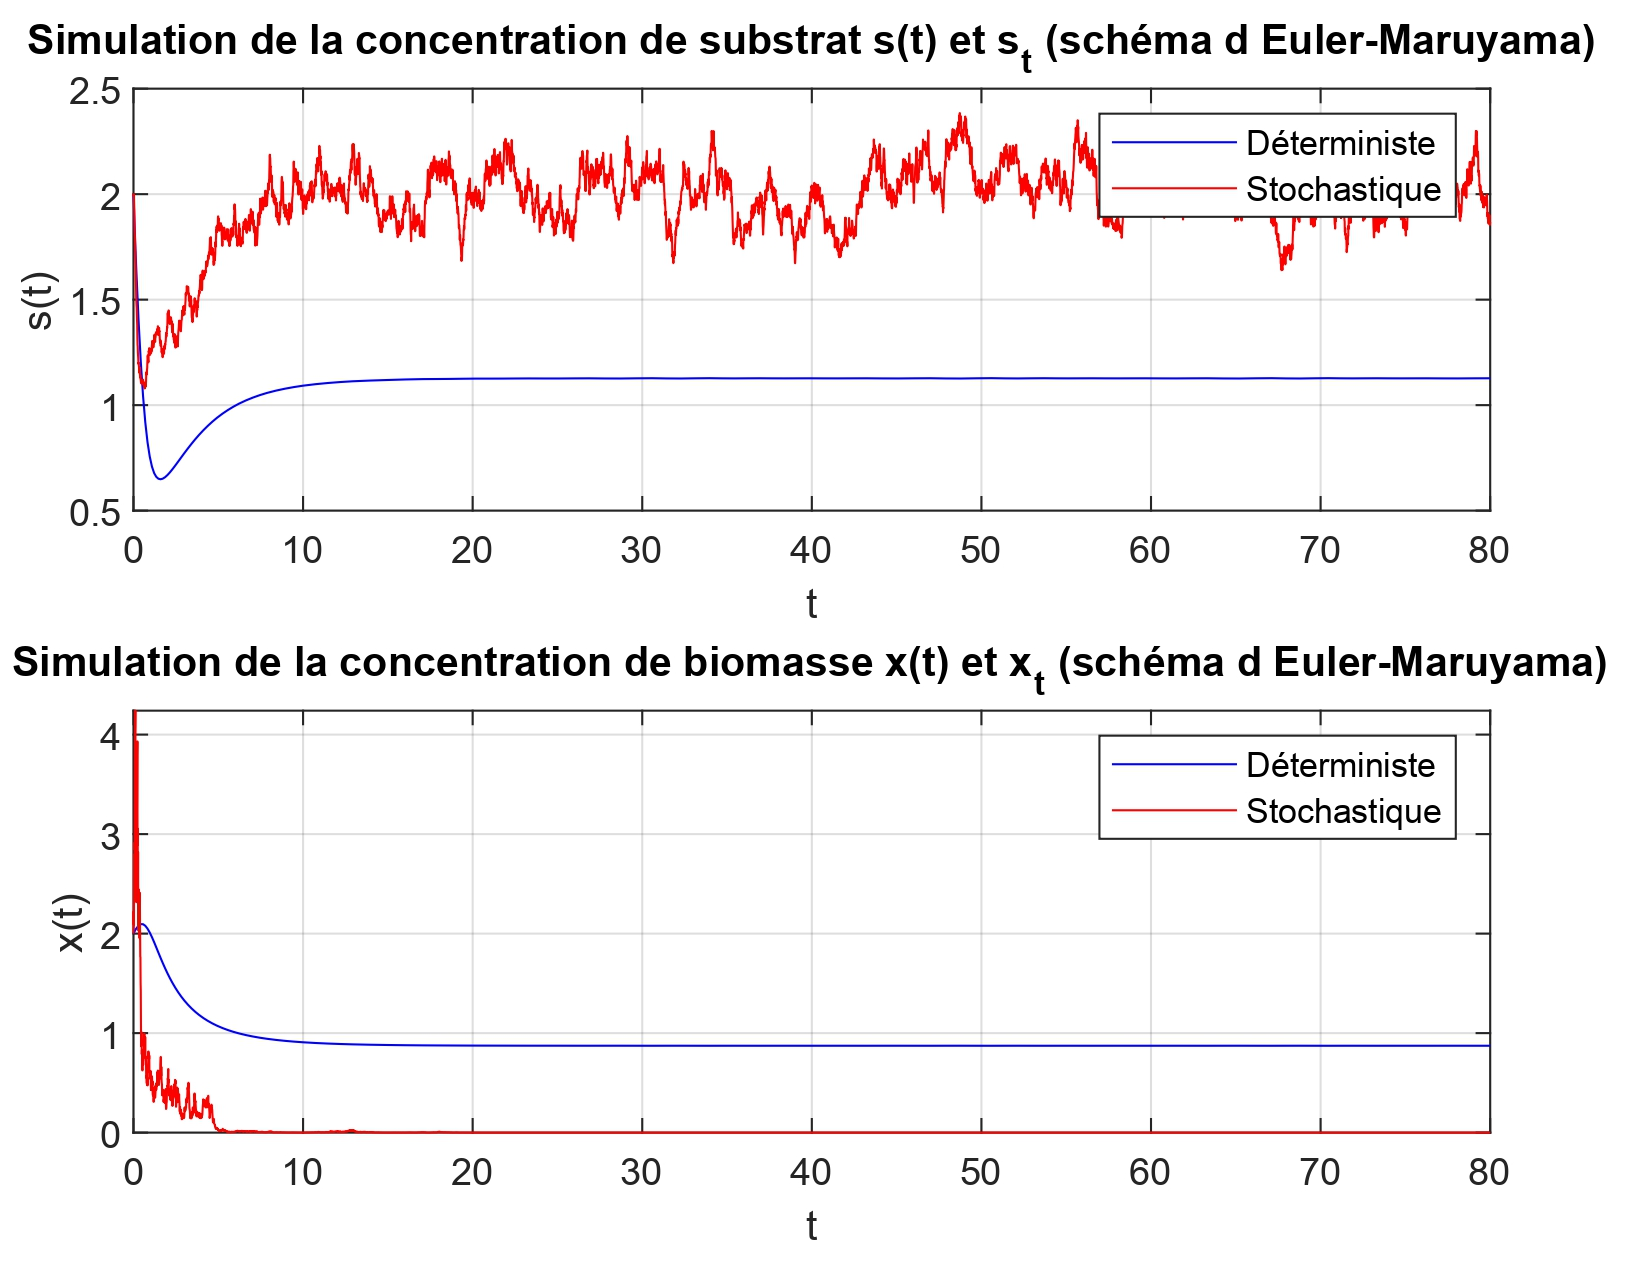
\includegraphics[width=1.05\textwidth]{C4_page-0001.png} 
	\caption{Solutions numériques pour le système \eqref{edssn} et le système déterministe correspondant \eqref{sigma} avec les paramètres principal \( D = 1 \), $\sigma_1=0.2 , \;et \;\; \sigma_2 = 1.1$.}
	\label{fig:fgure14}
\end{figure}
\newpage
Solutions numériques pour le système \eqref{edssn} et le système déterministe correspondant \eqref{sigma} avec les paramètres principal

\begin{center}
	\begin{tabular}{|c|c|c|c|c|}
		\hline
		\rowcolor{lightgray}
		{\bf La biomasse} &\footnotesize $D\downarrow < 1,\sigma_2 \downarrow <0.4 $ &\footnotesize $D \downarrow < 1 ,\sigma_2 \uparrow >1.6$ &\footnotesize $D\uparrow > 1.5 ,\sigma_2 \uparrow <0.3 $ &\footnotesize $D \uparrow > 2.4 , \sigma_2 \downarrow <0.03 $ \\
		\hline \hline
		Cas déterministe & Survie & Survie &\footnotesize  Extinction (lente) &\footnotesize Extinction (rapide) \\
		\hline 
		Cas stochastique & Survie &\footnotesize Extinction (rapide) &\footnotesize Extinction (lente) &\footnotesize Extinction (rapide)\\
		\hline
	\end{tabular}
	\captionof{table}{Effets du taux de dilution et stochasticité sur la survie-extinction de la biomasse.}
	\label{tab2}
\end{center}
Le tableau montre comment la biomasse se comporte avec l'atténuation et diverses fluctuations dans des contextes déterministes et stochastiques. Les systèmes stochastiques sont plus sensibles aux fluctuations environnementales élevées, ce qui peut conduire à une extinction rapide, tandis que les systèmes déterministes montrent une plus grande résilience dans certaines conditions.
 \chapter{Deuxième construction du modèle stochastique}
 Les systèmes réels, comme les chémostats, sont souvent sujets à des variations et des incertitudes. Ces variations peuvent provenir de différentes sources, telles que des fluctuations environnementales, des variations dans les taux de dilution, des erreurs de mesure ou des fluctuations dans la concentration d'entrée de substrat. Le modèle déterministe ne prend pas en compte ces fluctuations et suppose que toutes les variables évoluent de manière parfaitement prévisible.\\
 
 Pour modéliser ces fluctuations, nous introduisons un terme de bruit stochastique dans le modèle. Ce bruit peut être représenté par un processus de Wiener \(B(t)\), qui modélise des fluctuations aléatoires continues. En particulier, nous modélisons la dilution \(D\) comme une quantité fluctuante autour d'une valeur moyenne \(D_0\) avec une composante stochastique :
 
 \[ D = D_0 + \sigma \xi \]
 où \(\xi dt = dB(t)\) et \(\sigma\) est un paramètre qui mesure l'intensité du bruit.\\
 
 En ajoutant ce terme stochastique, nous transformons les équations déterministes en équations différentielles stochastiques. L'ajout du bruit stochastique affecte les équations de la manière suivante :
 
 1. Équation pour \(s(t)\) :
 \[
 ds(t) = \left( D \left(S_{in} - s(t)\right) - \mu(s(t)) x(t) \right) dt 
 \]
 En substituant \(D\) par \(D_0 + \sigma \xi\), nous obtenons :
 \[
 ds_t = \left( D_0 \left(S_{in} - s_t\right) - \mu(s_t) x_t \right) dt + \sigma \left(S_{in} - s_t\right) dB(t)
 \]
 
 2. Équation pour \(x(t)\) :
 \[
 dx(t) = \left( (\mu(s(t)) - D) x(t) \right) dt
 \]
 En substituant \(D\) par \(D_0 + \sigma \xi\), nous obtenons :
 \[
 dx_t = \left( (\mu(s_t) - D_0) x_t \right) dt - \sigma x_t dB(t)
 \]
 Ces transformations prennent en compte l'effet du bruit sur les taux de variation de \(s_t\) et \(x_t\), en incorporant des termes dépendants de \(dB(t)\), qui représentent les fluctuations aléatoires.\\
 Ainsi, les équations différentielles stochastiques résultantes sont :
 
 \begin{equation}\label{edss}
 	\begin{cases}
 		ds_t = \left( D_0 \left(S_{in} - s_t\right) - \mu(s_t) x_t \right) dt + \sigma \left(S_{in} - s_t\right) dB(t) \\
 		dx_t = (\mu(s_t) - D_0) x_t  dt - \sigma x_t dB(t) \\
 		s_0 = s_0 \\
 		x_0 = x_0
 	\end{cases}
 \end{equation}
 
 Ces équations permettent de modéliser le comportement du chémostat en prenant en compte les fluctuations stochastiques, offrant ainsi une représentation plus réaliste des dynamiques du système.
 \section{Existence et unicité de la solution }
 \begin{théorème}{Existence et unicité de la solution}{}
 	Pour tout $(s_0, x_0) \in \mathbb{R}_+^2$, il existe une unique solution $(s_t, x_t)$ de système \eqref{edss} définie pour tout $t \geq 0$ presque sûrement.
 \end{théorème}
 \begin{proof}
 	Pour simplifier les calculs, nous pouvons écrire le système d'équations différentielles stochastiques sous une forme matricielle compacte:
 	\begin{equation}\label{ds1}
 		dY_t = f(Y_t)dt + g(Y_t)dB(t) 
 	\end{equation}
 	
 	Avec \( Y_t = (s_t, x_t) \)
 	$$
 	\begin{array}{rcl}
 		f:\mathbb{R}^2 &\to& \mathbb{R}^2\\
 		Y &\mapsto &f(Y)=\begin{pmatrix}
 			D_0(S_{in}-s) - \mu(s)x \\
 			(\mu(s)-D_0)x
 		\end{pmatrix}
 	\end{array}
 	$$
 	$$
 	\begin{array}{rcl}
 		g:\mathbb{R}^2 &\to& \mathbb{R}^2\\
 		Y &\mapsto &g(Y)=\begin{pmatrix}
 			-\sigma ( S_{in}-s) \\
 			-\sigma x
 		\end{pmatrix}
 	\end{array}
 	$$
 	i) $\blacklozenge$ Vérifions la premier condition du théorème d'existence \ref{theorem:existancesto} :\\
 	On a déjà monter que $f$ est lipschitzienne dans le cas déterministe, donc il existe $k\geqslant 0$ tel que: $\|f(Y)-f(Z)\| \leq k \|Y-Z\|$ pour tout $Y,Z \in \mathbb{R}^2_+$.
 	Pour $g_1$ et $g_2$ on a:\\
 	Soient $Y=(x,y), \;Z=(a, b) \in \mathbb{R}^2_+$ 
 	$$ 
 	\begin{aligned}
 		\|g(Y)-g(Z)\|&=|\sigma s -\sigma a|+|\sigma x -\sigma b|\\
 		&=|\sigma|( | (s -a)|+| (x -b)|\\
 		&= |\sigma| \|Y-Z\|
 	\end{aligned}
 	$$
 	
 	Ainsi 
 	$$
 	\|f(Y)-f(Z)\|+\|g(Y)-g(Z)\|\leq (k+|\sigma|) \|Y-Z\| 
 	$$
 	pour tout $\;Y,Z \in \mathbb{R}^2_+$\\
 	ii) $\blacklozenge$ Pour la deuxième condition du théorème d'existence \ref{theorem:existancesto}, on commence par \( g \). Soit \( Y \in \mathbb{R}^2_+ \), on a :
 	\begin{align*}
 		\|g(Y)\| &= |\sigma( S_{in}-s)|+|\sigma x| \\
 		&\leqslant |\sigma S_{in}|+|\sigma s|+|\sigma x|\\
 		&=|\sigma S_{in}|+|\sigma| \|Y\|\\
 		&\leqslant |\sigma| Max(S_{in},1)(1+\|Y\|)
 	\end{align*}
 	Et pour $f$ on a $\|f(Y)\|=|D_0(S_{in}-s) - \mu(s)x|+|(\mu(s)-D_0) x|$
 	\begin{align*}
 		|D_0(S_{in}-s) - \mu(s)x| & = |D_0 S_{in}-D_0 s - \mu(s)x| \\
 		& \leqslant D_0 S_{in}+|D_0 s + \mu(s)x| \\
 		& \leqslant D_0 S_{in}+(D_0+\mu_{\text{max}})\|Y\| \\
 		& = (D_0 S_{in}+D_0+\mu_{\text{max}})(1+\|Y\|)
 	\end{align*}
 	\begin{align*}
 		|(D_0 - \mu(s))x| & = |(D_0 - \mu(s))|x| \\
 		& \leqslant (D_0 + \mu_{max})|x| \\
 		& \leqslant (D_0 + \mu_{max})(1+\|Y\|)
 	\end{align*}
 	donc 
 	$\|f(Y)\|\leqslant L(1+\|Y\|)$ et $L=D_0 S_{in}+D_0+\mu_{\text{max}}$ (en utiliser toujours le fait que \(|s| \)  et \(|x| \) est bornée par \( 1 + \|Y\| \). Ainsi 
 	$$
 	\|f(Y)\|+\|g(Y)\|\leq (L+|\sigma| Max(S_{in},1))\left( 1+ \|Y\| \right) 
 	$$
 	La deuxième condition du théorème d'existence \ref{theorem:existancesto} est satisfaite. Alors il existe $T>0 $ et un processus $(s_t, x_t)_{t \in [0,T[}$ unique, continue et adapté à la filtration, qui satisfait l'équation \eqref{ds1}.
 	Pour prouver que la solution est globale, il suffit de démontrer que le temps de blow-up \(\tau_e\) est infini presque sûrement (p.s.).\\
 	
 	en effet 
 	\[
 	\begin{aligned}
 		d(s_t+x_t)=&[D(S_{in}-s_t)-D x_t]dt \\
 		&=D[S_{in}-s_t-x_t]dt\\
 		&=D_0[S_{in}-s_t-x_t]dt+ \sigma [S_{in}-s_t-x_t]dB_t
 	\end{aligned}
 	\]
 	on pose $z_t=S_{in}-s_t-x_t$ alors :
 	\[
 	\begin{aligned}
 		dz_t=&-D_0 z_tdt- \sigma z_tdB_t\\
 		&=-z_t[D_0dt + \sigma dB_t]
 	\end{aligned}
 	\]
 	
 	Alors d'après la formule d'Itô, nous avons :
 	
 	\[
 	\begin{aligned}
 		d(\log(z_t)) &= \frac{dz_t}{z_t} - \frac{1}{2}\sigma^2 dt\\
 		&=-[D_0dt + \sigma dB_t] - \frac{1}{2}\sigma^2 dt\\
 		&=-[D_0+ \frac{1}{2}\sigma^2 ]dt - \sigma dB_t
 	\end{aligned}
 	\]
 	
 	
 	Alors,
 	\[
 	\log(z_t) - \log(z_0) = -\int_0^t [D_0+ \frac{1}{2}\sigma^2 ]dr - \int_0^t  \sigma dB_r,
 	\]
 	
 	\[
 	\Rightarrow \;\; z_t = z_0 e^{- [D_0+ \frac{1}{2}\sigma^2 ] t - \sigma B_t}.
 	\]
 	\[
 	\Rightarrow \;\; s_t+x_t =S_{in}-(S_{in}-s_0-x_0) e^{- [D_0+ \frac{1}{2}\sigma^2 ] t - \sigma B_t}.
 	\]
 	puisque $\sup\limits_{s \in [0, t[} \|s_s+x_s\|<\infty $ pour tout $t \geqslant 0$ 
 	
 	Le temps de blow-up \( \tau_e \) est défini comme le premier moment où \( s_t + x_t \) devient infini. Cela implique :
 	
 	\[ \tau_e = \infty. \]
 	
 	et donc \(s_t\) et \(x_t\) est globale c'est-à-dire définis pour tout \( t \geqslant 0\)
 \end{proof}
 
 
 \begin{Proposition}{}\label{système1}
 	Pour tout \((s_0, x_0) \in \mathbb{R}_+^2\), on a \(x_t \geqslant 0\) p.s. et \(\mathbb{P}( s_t \geqslant 0 \;\, \forall t \geq 0) < 1\).
 	
 \end{Proposition}
 \begin{proof} 
 	Puisque nous avons
 	
 	\[
 	dx_t = \left((\mu(s_t) - D_0)x_t\right) dt - \sigma x_t dB(t),
 	\]
 	
 	alors d'après la formule d'Itô, nous avons :
 	
 	\[
 	\begin{aligned}
 		d(\log(x_t)) &= \frac{dx_t}{x_t} + \frac{1}{2}(\sigma x_t)^2 \frac{-1}{x_t^2} dt \\
 		&= \left((\mu(s_t) - D_0) - \frac{\sigma^2}{2}\right) dt - \sigma dB(t).
 	\end{aligned}
 	\]
 	
 	Alors,
 	
 	\[
 	\log(x_t) - \log(x_0) = \int_0^t \left((\mu(s_r) - D_0) - \frac{\sigma^2}{2}\right) dr - \int_0^t \sigma dB(r),
 	\]
 	
 	\[
 	\Rightarrow \;\; x_t = x_0 e^{\int_0^t (\mu(s_r) - D_0) dr - \frac{\sigma^2}{2} t - \sigma B(t)}.
 	\]
 	
 	Donc, si \(x_0\) est positive, le processus \((x_t)_{t\geqslant0 }\) reste positive.\\
 	
 	En suppose que \((s_t)_{t\geqslant0 }\) est positive p.s.\\
 	Pour \( x_0 = 0 \), alors \( x_t = 0 \) p.s.
 	
 	Donc
 	\[
 	s_t = S_{in} - (S_{in} - s_0) e^{-(D_0 + \frac{\sigma^2}{2})t - \sigma B_t}.
 	\]
 	
 	On pose \( S_{in} = 2 s_0 \)
 	
 	\[
 	s_t = 2 s_0 - s_0 e^{-(D_0 + \frac{\sigma^2}{2})t - \sigma B_t}
 	\]
 	\[
 	= s_0 \left( 2 - e^{-(D_0 + \frac{\sigma^2}{2})t - \sigma B_t} \right).
 	\]
 	
 	\( s_t \geq 0 \) implique
 	\[
 	2 - e^{-(D_0 + \frac{\sigma^2}{2})t - \sigma B_t} \geq 0 \;\;\;(s_0 \geqslant 0).
 	\]
 	
 	Mais
 	\[
 	\mathbb{P} \left( 2 - e^{-(D_0 + \frac{\sigma^2}{2})t - \sigma B_t} \geq 0 \right) < 1.
 	\]
 	On a
 	\[
 	\begin{aligned}
 		\mathbb{P} \left( 2 - e^{-(D_0 + \frac{\sigma^2}{2})t - \sigma B_t} \geq 0 \right) &=  \mathbb{P} \left( 2 \geqslant e^{-(D_0 + \frac{\sigma^2}{2})t - \sigma B_t}  \right)\\
 		&= \mathbb{P} \left( ln(2) \geqslant -(D_0 + \frac{\sigma^2}{2})t - \sigma B_t  \right)\\
 		&= \mathbb{P} \left( B_t \geqslant \frac{-ln(2)  -(D_0 + \frac{\sigma^2}{2})t} {\sigma}  \right)\\
 		&=1-  \mathbb{P} \left( B_t < \frac{-ln(2)  -(D_0 + \frac{\sigma^2}{2})t} {\sigma}  \right)\\
 		&<1
 	\end{aligned}
 	\]
 	car \(\mathbb{P} \left( B_t < \frac{-\ln(2) - (D_0 + \frac{\sigma^2}{2})t}{\sigma} \right) > 0\) pour tout \(t > 0\).
 	
 	Ainsi, il existe un \(\Omega^\prime\) tel que \(\mathbb{P}(\Omega^\prime) > 0\) et \(s_t(\omega) < 0\) pour tout \(\omega \in \Omega^\prime\) et $t>0$ (Absurde).\\
 	Donc  \(\mathbb{P}( s_t \geqslant 0 \;\, \forall t \geq 0) < 1\).
 \end{proof}
\begin{remarque}{}\label{re}
	Puisque la solution $s_t$ n'est pas positive presque sûrement, nous perdons également la bornitude de $s_t$ et $x_t$.
\end{remarque}

 
 Dans le cadre d'un chémostat, le taux de dilution \(D\) joue un rôle crucial. Ce taux représente la vitesse à laquelle le milieu de culture est renouvelé, c'est-à-dire la vitesse à laquelle des nutriments frais sont ajoutés et le mélange de culture (contenant les micro-organismes, les déchets et les nutriments résiduels) est retiré. En modélisant ce système, il est courant d'introduire un terme stochastique pour capturer les fluctuations aléatoires qui peuvent survenir.
 
 Dans cette construction, nous avons posé \(D = D_0 + \sigma \xi\), où \(D_0\) est le taux de dilution nominal (ou moyen), \(\sigma\) est l'amplitude du bruit, et \(\xi\) est un processus stochastique, souvent supposé suivre une distribution normale \(\mathcal{N}(0,1)\). Cela signifie que \(\xi\) peut prendre des valeurs aussi bien positives que négatives.
 
 Le problème se pose lorsque le bruit \(\xi\) prend une valeur négative suffisamment grande, entraînant une dilution \(D\) négative :
 \[ D = D_0 + \sigma \xi < 0. \]
 Une dilution négative n'a pas de sens physique dans le contexte d'un chémostat, car cela impliquerait que le milieu de culture est ajouté au système au lieu d'être retiré, ce qui est contraire à la définition de la dilution. En termes pratiques, une dilution négative pourrait être interprétée comme une croissance non contrôlée du volume de la culture, ce qui n'est pas réaliste et pourrait entraîner des instabilités dans la modélisation de la dynamique microbienne.
 
 En conclusion, bien que l'introduction d'un terme stochastique dans le taux de dilution \(D\) soit une approche valide pour capturer les fluctuations aléatoires, il est essentiel de s'assurer que cette modélisation n'entraîne pas des valeurs non physiques de \(D\). Cela nécessite une gestion appropriée du bruit \(\xi\) pour maintenir la validité et la stabilité du modèle.
\section{Application numérique }%du deuxième modèle stochastique
Pour illustrer les résultats analytiques des chapitre 2 et 4, nous devons obtenir des solutions approchées du système stochastique \eqref{edss} et aussi le cas déterministe \eqref{1.2} avec des valeurs initiales et des paramètres donnés, via des méthodes numériques et des algorithmes pouvant être implémentés par Matlab. En raison du mouvement brownien et des termes de bruit $\sigma(S_{in} - s_t) dB(t)$ et $-\sigma x_t dB(t)$, nous utilisons la méthode d'Euler-Maruyama pour obtenir les solutions approchées du modèle de chémostat stochastique.

Nous considérons le système stochastique suivant :

\begin{equation}\label{edssn}
\begin{cases}
ds_t = \left( D_0 \left(S_{in} - s_t\right) - \mu(s_t) x_t \right) dt + \sigma \left(S_{in} - s_t\right) dB(t) \\
dx_t = \left( (\mu(s_t) - D_0) x_t \right) dt - \sigma x_t dB(t) \\
s_0 = S_0 \\
x_0 = X_0
\end{cases}
\end{equation}

Pour obtenir des solutions approchées de ce système, nous utilisons la méthode d'Euler-Maruyama. La discrétisation par la méthode d'Euler-Maruyama pour ce système est formulée comme suit :

\begin{equation}\label{matlab1}
\begin{cases}
s_{i+1} = s_i + \left( D_0 (S_{in} - s_i) - \mu(s_i) x_i \right) \Delta t + \sigma (S_{in} - s_i) (B_{t_{i+1}} - B_{t_i}) \\
x_{i+1} = x_i + \left( (\mu(s_i) - D_0) x_i \right) \Delta t - \sigma x_i (B_{t_{i+1}} - B_{t_i}) \\
\end{cases}
\end{equation}

où 
\begin{itemize}
	\item \( s_{i+1} \) et \( x_{i+1} \) : Les valeurs des variables \( s \) et \( x \) à l'instant \( t_{i+1} \).
	\item \( \Delta t \) : L'intervalle de temps entre \( t_i \) et \( t_{i+1} \).
	\item \( B_{t_{i+1}} - B_{t_i} \) : L'incrément du mouvement brownien entre \( t_i \) et \( t_{i+1} \), modélisant l'effet aléatoire.
\end{itemize}
De cette manière, les solutions approchées (les résultats de performance de \eqref{matlab1} de Matlab) convergeront très rapidement vers les solutions explicites du système stochastique \eqref{edss}.
\begin{exemple}{}
D'après la proposition \ref{système1}, nous nous attendons à ce que, sous certaines conditions appropriées, le système stochastique \eqref{edssn} vérifie \(x_t \geqslant 0\) p.s. et \(\mathbb{P}(s_t \geqslant 0 \;\, \forall t \geq 0) < 1\). Choisissons les valeurs initiales \((s_0, x_0) = (3.02, 1)\) et supposons que les paramètres dans \eqref{edssn} sont donnés par \(m = 2\), \(S_{in} = 1\), \(a = 1\), et \(K = 1.1\).

Dans la proposition \ref{système1}, toutes les conditions sont satisfaites. Nous en concluons donc que \(x_t \geqslant 0\) p.s. et \(\mathbb{P}(s_t \geqslant 0 \;\, \forall t \geq 0) < 1\) (voir les deux sous-graphiques dans la figure \ref{fig:fgure1}). Les simulations numériques dans la figure \ref{fig:fgure1} soutiennent clairement cette conclusion.
\end{exemple}
\begin{figure}[h]
	\centering
	\begin{minipage}{0.48\textwidth}
		\centering
		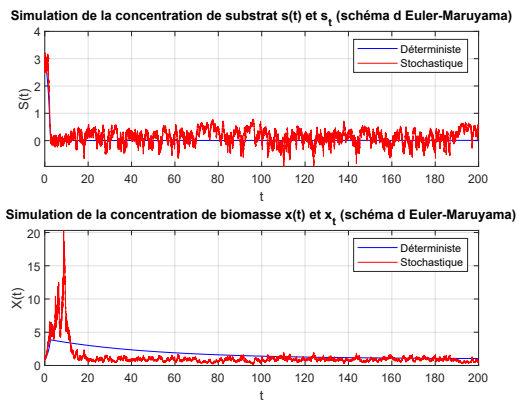
\includegraphics[width=\textwidth]{e3.png}
		\caption*{ $\sigma = 0.5$.}
	%	\label{fig:figure1a}
	\end{minipage}
	\hfill
	\begin{minipage}{0.48\textwidth}
		\centering
		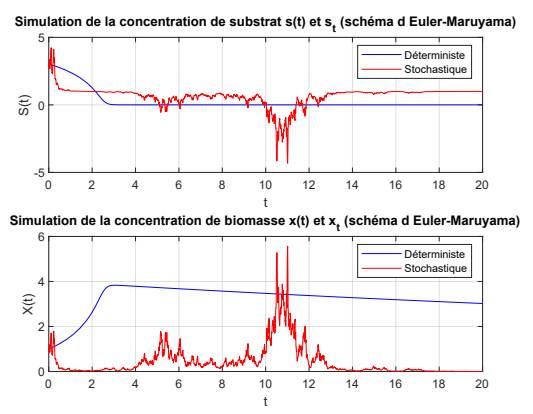
\includegraphics[width=\textwidth]{e4.png}
		\caption*{ $\sigma = 1.5$.}
		%\label{fig:figure1b}
	\end{minipage}
	\caption{Solutions numériques pour le système \eqref{edssn} et le système déterministe correspondant \eqref{1.2} avec les paramètres principal \(D= D_0 = 0.002 \), $s_0=3.02$ et $x_0=1$.}
   \label{fig:fgure1}
\end{figure}
\begin{exemple}{}
On remarque dans cet exemple que si l'intensité du bruit est très faible, le processus \(s_t\) reste également positif mais pas presque sûrement. Les deux sous-figures de la figure \ref{fig:fgure2} soutiennent cette observation.

\end{exemple}
\begin{figure}[h]
	\centering
	\begin{minipage}{0.48\textwidth}
		\centering
		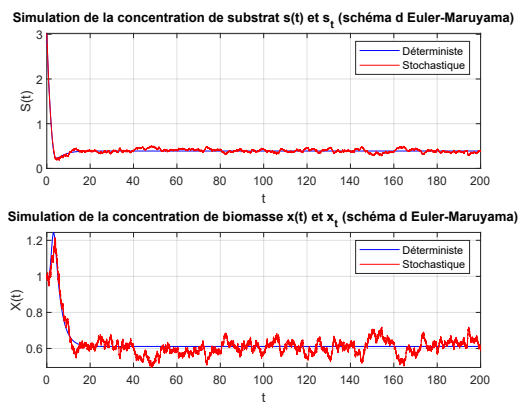
\includegraphics[width=\textwidth]{e1.png}
		\caption*{$D= D_0 = 0.5$ et $\sigma = 0.05$.}
		%	\label{fig:figure1a}
	\end{minipage}
	\hfill
	\begin{minipage}{0.48\textwidth}
		\centering
		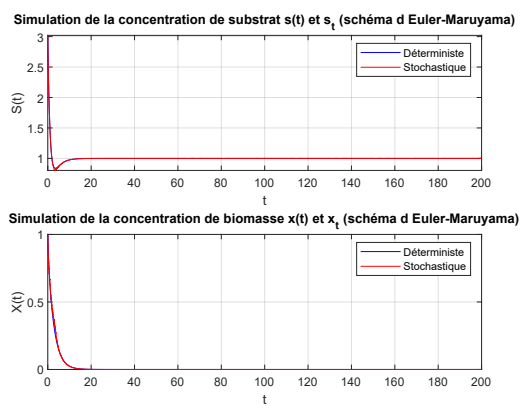
\includegraphics[width=\textwidth]{e2.png}
		\caption*{$D= D_0 = 1$et $\sigma = 0.05$.}
		%\label{fig:figure1b}
	\end{minipage}
	\caption{Solutions numériques pour le système \eqref{edssn} et le système déterministe correspondant \eqref{1.2} avec les paramètres principal, $s_0=3.02$ et $x_0=1$.}
	\label{fig:fgure2}
\end{figure}
\begin{exemple}{}
	Dans la remarque \ref{re}, nous avons obtenu que les solutions $s_t$ et $x_t$ ne sont pas bornées. La solution numérique confirme ce résultat, comme illustré dans la figure \ref{fig:fgure5}, avec des paramètres $m=5$ et $\sigma=1.5$.
\end{exemple}


\begin{figure}[h]
	\centering
	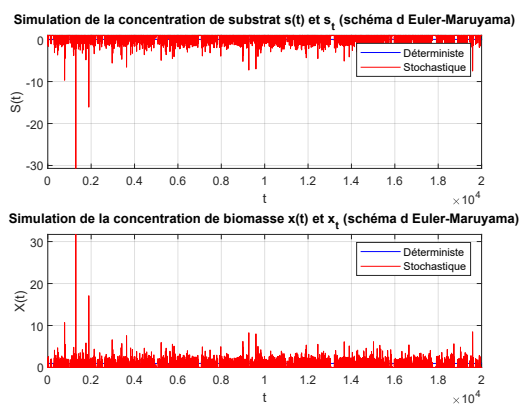
\includegraphics[width=1.05\textwidth]{e5.png} 
	\caption{Solutions numériques pour le système \eqref{edssn} et le système déterministe correspondant \eqref{1.2} avec les paramètres principal \(D= D_0 = 0.2 \), $s_0=0$ et $x_0=1$.}
	\label{fig:fgure5}
\end{figure}


\chapter*{Conclusion et perspective}
Dans ce mémoire, nous avons exploré le modèle du chémostat sous deux angles : le cas déterministe et le cas stochastique. Nous avons d'abord établi les bases du modèle déterministe, où les équations différentielles ordinaires décrivent l'évolution des concentrations de substrat et de biomasse dans un environnement contrôlé. Ce cadre a permis de bien comprendre la dynamique du système en conditions idéales et d'identifier les points d'équilibre et leur stabilité.\\
\vspace*{0.1cm}

Ensuite, nous avons étendu le modèle au cas stochastique pour intégrer les incertitudes et les fluctuations inhérentes aux systèmes biologiques réels. Deux constructions distinctes ont été proposées :

1. Première Construction : Nous avons ajouté des termes stochastiques de type bruit multiplicatif $ + \sigma_1 s(t) \xi_1 $ dans l'équation du substrat et $ + \sigma_2 s(t) \xi_2 $ dans l'équation de la biomasse. Cette approche a permis de capturer les fluctuations aléatoires autour des concentrations de substrat et de biomasse. Les résultats théoriques ont été validés par des simulations numériques, démontrant que les prédictions du modèle stochastique concordent bien avec les observations empiriques.

2. Deuxième Construction : Nous avons considéré une dilution stochastique $ D = D_0 + \sigma \xi $, introduisant ainsi une variabilité dans le taux de dilution. Cependant, cette formulation a mené à un problème de faisabilité physique, car la dilution pouvait prendre des valeurs négatives, ce qui n'est pas réaliste pour un chémostat. Ce problème souligne les défis de la modélisation stochastique et la nécessité de formuler des hypothèses qui respectent les contraintes physiques du système.\\
\vspace*{0.1cm}

Pour résoudre le problème de la dilution négative, nous proposons d'utiliser une formulation exponentielle pour la dilution :
\[ D = D_0 e^{\sigma B_t} \]
où \( B_t \) est un processus de Wiener (ou mouvement brownien). Cette approche garantit que le taux de dilution reste toujours positif, respectant ainsi les contraintes physiques du système.\\
\vspace*{0.1cm}

En conclusion, l'utilisation d'une dilution stochastique exponentielle offre une solution élégante au problème de la dilution négative et ouvre de nouvelles perspectives pour la modélisation des systèmes biologiques complexes.
\newpage
\chapter*{Code MATLAB}
\small
{\scriptsize
	\setstretch{0.6}
	{\bf Code MATLAB pour le dixième modèle avec un mouvement brownien unidimensionnel}
	\begin{lstlisting}
		% Parametres du modele
		D = 1,D0 = 1;       % Debit de dilution
		S_in = 3.0;  % Concentration de substrat en entree
		a = 1.0;      % Parametre de saturation
		M = 2;      % Taux de croissance maximal
		k = 0.1;     % Parametre de saturation non lineaire
		sigma = 0.72; % Exemple de valeur
		s0 = 2.0, x0 = 2.0;  % Concentration initiale de substrat et de biomasse
		y0 = [s0; x0];
		t_span = [0 100];   % Intervalle de temps pour la simulation
		% Resolution du systeme d'EDOs (methode deterministe)
		[t_d, y_d] = ode45(@(t, y) model(t, y, D, S_in, M, a, k), t_span, y0);
		% Extraction des resultats pour la methode deterministe
		s_d = y_d(:, 1);
		x_d = y_d(:, 2);
		% Parametres de simulation
		T = 100.0;    % Temps total de simulation
		dt = 0.01;   % Pas de temps
		N = T/dt;    % Nombre de points de temps
		% Initialisation des tableaux pour stocker les solutions stochastiques
		s_e = zeros(N, 1);
		x_e = zeros(N, 1);
		t_s = linspace(0, T, N);
		% Conditions initiales
		s_e(1) = s0;
		x_e(1) = x0;
		% Simulation avec la methode d'Euler-Maruyama
		for i = 2:N
		dB = sqrt(dt) * randn;
		mu_e = (M * s_e(i-1)) / (a + s_e(i-1) + k * s_e(i-1)^2);
		ds_e = (D0 *(S_in-s_e(i-1))-mu_e*x_e(i-1))*dt+sigma*(S_in-s_e(i-1))*dB;
		dx_e = (mu_e - D0) * x_e(i-1) * dt - sigma * x_e(i-1) * dB;
		s_e(i) = s_e(i-1) + ds_e;
		x_e(i) = x_e(i-1) + dx_e;
		end
		figure;  % Trace des resultats
		% Trace de la concentration de substrat (s)
		subplot(2, 1, 1);
		plot(t_d, s_d, 'b', 'DisplayName', 'Deterministe');
		hold on;
		plot(t_s, s_e, 'r', 'DisplayName', 'Stochastique');
		xlabel('t');
		ylabel('S(t)');
		legend;
		title('Simulation de la concentration de substrat S(t)');
		grid on;
		% Trace de la concentration de biomasse (x)
		subplot(2, 1, 2);
		plot(t_d, x_d, 'b', 'DisplayName', 'Deterministe');
		hold on;
		plot(t_s, x_e, 'r', 'DisplayName', 'Stochastique');
		xlabel('t');
		ylabel('X(t)');
		legend;
		title('Simulation de la concentration de biomasse X(t)');
		grid on;
		% Fonction pour le systeme d'EDOs (methode deterministe)
		function dydt = model(t, y, D, S_in, m, a, k)
		s = y(1);
		x = y(2);
		mu_s = (m * s) / (a + s + k * s^2);
		ds_dt = D * (S_in - s) - mu_s * x;
		dx_dt = (mu_s - D) * x;
		dydt = [ds_dt; dx_dt];
		end
	\end{lstlisting}
}
\newpage
\small
{\scriptsize
	\setstretch{0.6}
	{\bf Code MATLAB pour le première modèle avec deux mouvements browniens indépendants}
	\begin{lstlisting}
		% Parametres du modele
		D = 1;      % Debit de dilution 
		S_in = 2.0;  % Concentration de substrat en entree
		a = 1.0;      % Parametre de saturation
		M = 2;      % Taux de croissance maximal
		k = 0.1;     % Parametre de saturation non lineaire
		sigma_1 = 0.03;
		sigma_2 = 1.01;  % Exemple de valeur
		% Conditions initiales
		s0 = 2.0;  % Concentration initiale de substrat
		x0 = 2.0;  % Concentration initiale de biomasse
		y0 = [s0; x0];
		% Intervalle de temps pour la simulation
		t_span = [0 80];
		% Resolution du systeme d'EDOs (methode deterministe)
		[t_d, y_d] = ode45(@(t, y) model(t, y, D, S_in, M, a, k), t_span, y0);
		% Extraction des resultats pour la methode deterministe
		s_d = y_d(:, 1);
		x_d = y_d(:, 2);
		% Parametres de simulation
		T = 80.0;    % Temps total de simulation
		dt = 0.01;   % Pas de temps
		N = T/dt;    % Nombre de points de temps
		% Initialisation des tableaux pour stocker les solutions stochastiques
		s_e = zeros(N, 1);
		x_e = zeros(N, 1);
		t_s = linspace(0, T, N);
		% Conditions initiales
		s_e(1) = s0;
		x_e(1) = x0;
		% Simulation avec la methode d'Euler-Maruyama
		for i = 2:N
		dB1 = sqrt(dt) * randn;
		dB2 = sqrt(dt) * randn;
		mu_e = (M * s_e(i-1)) / (a + s_e(i-1) + k * s_e(i-1)^2);
		ds_e = (D *(S_in-s_e(i-1))-mu_e*x_e(i-1))*dt + sigma_1*s_e(i-1)*dB1;
		dx_e = (mu_e - D) * x_e(i-1) * dt + sigma_2 * x_e(i-1) * dB2;
		s_e(i) = s_e(i-1) + ds_e;
		x_e(i) = x_e(i-1) + dx_e;
		end
		% Trace des resultats
		figure;
		% Trace de la concentration de substrat (s)
		subplot(2, 1, 1);
		plot(t_d, s_d, 'b', 'DisplayName', 'Deterministe');
		hold on;
		plot(t_s, s_e, 'r', 'DisplayName', 'Stochastique');
		xlabel('t');
		ylabel('s(t)');
		legend;
		title('Simulation de la concentration de substrat s(t) et s_t (schema d Euler-Maruyama)');
		grid on;
		% Trace de la concentration de biomasse (x)
		subplot(2, 1, 2);
		plot(t_d, x_d, 'b', 'DisplayName', 'Deterministe');
		hold on;
		plot(t_s, x_e, 'r', 'DisplayName', 'Stochastique');
		xlabel('t');
		ylabel('x(t)');
		legend;
		title('Simulation de la concentration de biomasse x(t) et x_t (schema d Euler-Maruyama)');
		grid on;
		% Fonction pour le systeme d'EDOs (methode deterministe)
		function dydt = model(t, y, D, S_in, m, a, k)
		s = y(1);
		x = y(2);
		mu_s = (m * s) / (a + s + k * s^2);
		ds_dt = D * (S_in - s) - mu_s * x;
		dx_dt = (mu_s - D) * x;
		dydt = [ds_dt; dx_dt];
		end
		
	\end{lstlisting}
}
\newpage
\begin{thebibliography}{Dillo 83}
	\addcontentsline{toc}{chapter}{Bibliographie}
	
	\bibitem{c} Chabour Ourida. \emph{Stabilisation des systèmes non linéaires}, 31 mars 2000.
	\bibitem{d} Harmand Jérôme, Claude Lobry, Alain Rapaport, Tewfik Sari. \emph{The Chemostat, Mathematical Theory of Microorganism Cultures}, Wiley-ISTE; 1ère édition, 7 août 2017.
	\bibitem{art2} Ikeda Nobuyuki, Shinzo Watanabe. \emph{A comparison theorem for solutions of stochastic differential equations and its applications}, Osaka J. Math, 1977.
	\bibitem{book} Ikeda Nobuyuki, Shinzo Watanabe. \emph{	Stochastic Differential Equations and Diffusion Processes}.
	\bibitem{rafail} Khasminskii Rafail. \emph{Stochastic Stability of Differential Equations}, Springer-Verlag Berlin Heidelberg, 2012.
	\bibitem{c} Léonard Gallardo. \emph{Mouvement brownien et calcul d'Itô.}
	\bibitem{F} Rouvière François. \emph{Petit guide de calcul différentiel à l'usage de la licence et de l'agrégation}, Cassini, 3\textsuperscript{ème} édition, 2009.
	\bibitem{w} Wang Liang, Daqing Jiang, Gail S. K. Wolkowicz, Donal O’Regan. \emph{Dynamics of the stochastic chemostat with Monod-Haldane response function}, Scientific Reports, 20 September 2017.
	\bibitem{w1} Wang Liang, Daqing Jiang, Donal O’Regan. \emph{The periodic solutions of a stochastic chemostat model with periodic washout rate}.
	\bibitem{w2} Wang Liang, Daqing Jiang. \emph{ A note on the stationary distribution of the stochastic chemostat model with general response functions}.
	\bibitem{z}Zastawniak Tomasz, Zdzislaw Brzezniak. \emph{Basic Stochastic Processes}.
	

\end{thebibliography}
%\newpage

%%%%%%%%%%%%%%%%%%%%%%%%%%%%%%%%%%%%%%%%%%%%%%%%%%%%%%%%%%%%%%%%%%%%%%%%%%%%%%%%%%%%%%%%%%%%%%%%%%%%%%%%%%%%%%%%


%%%%%%%%%%%%%%%%%%%%%%%%%%%%%%%%%%%%%%%%%%%%%%%%les definition%%%%%%%%%%%%%%%%%%%
\begin{mycomment} 
	 Résumé du Mémoire
	
	Ce mémoire traite de l'analyse des systèmes différentiels déterministes et stochastiques appliqués au modèle de chémostat. Il est structuré en trois parties, chacune abordant des aspects spécifiques des équations différentielles et des modèles mathématiques utilisés pour décrire la dynamique des systèmes biologiques.
	
	La première partie se penche sur le modèle de chémostat déterministe. Elle détaille l'équation du chémostat et les propriétés mathématiques associées. Cette partie explore l'existence et l'unicité de la solution positive et examine les caractéristiques des taux de croissance de la biomasse. Elle inclut également des diagrammes opératoires pour illustrer le modèle et discute de la présence de biomasse dans l'alimentation.
	
	La deuxième partie présente la première construction du modèle stochastique du chémostat. Elle discute de l'existence et de l'unicité de la solution positive dans un contexte stochastique, examine l'extinction de la biomasse, et analyse la distribution stationnaire et l'ergodicité du modèle. Cette partie est consacrée à la simulation numérique du premier modèle stochastique. Elle permet de comparer les résultats des simulations déterministes et stochastiques, mettant en évidence les différences et les similitudes entre les deux approches.
	
	La dernière partie propose une deuxième construction du modèle stochastique et présente une application numérique de cette construction. Cette section vise à affiner et à améliorer la modélisation stochastique du chémostat.
	
	
	
	
\begin{théorème}{}
\end{théorème}
\begin{proof}
\end{proof}
\begin{définition}{}
\end{définition}
\begin{exemple}{}
\end{exemple}
\begin{remarque}{}
\end{remarque}
\begin{lemme}{}
\end{lemme} 
\begin{Proposition}{}
\end{Proposition}
\begin{corollaire}{}
\end{corollaire}
\begin{Propriété}{}
\end{Propriété}

%%%%%%%%%%%%%%%%%%%%%%%%%%%%%%%%%%%%%%%%%%%%%%%%%%%%%%%%%%%%%%%%%%%%%%%%%%%%%%%%%%%%%
\newpage
\begin{thebibliography}{Dillo 83}
\addcontentsline{toc}{chapter}{Bibliographie}

\bibitem{d}  Jérôme Harmand ,Claude Lobry , Alain Rapaport , Tewfik Sari .\emph{ The Chemostat, Mathematical Theory of Microorganism Cultures }, Wiley -ISTE; 1ère édition (7 août 2017).
\bibitem{c}  F. Rouvière. \emph{ Petit guide de calcul différentiel à l'usage de la licence et de l'agrégation.} Cassini, $3\textsuperscript{ème}$ édition, 2009 
\bibitem{c}  Léonard Gallardo. \emph{ Mouvement brownien et calcul d'Itô.}
\bibitem{c}  Ourida CHABOUR . Thèse \emph{Stabilisation des systèmes non linéaires,} 31 MARS 2000.
\bibitem{a}  Liang Wang,  Daqing Jiang, Gail S. K. Wolkowicz et Donal O’Regan .  \emph{Dynamics of the stochastic chemostat with Monod-Haldane response function.} Scientific Reports, 20 September 2017.
\bibitem{art2} NOBUYUKI IKEDA , SHINZO WATANABE.  \emph{A comparison theorem for solutions of stochastic differential equations and its applications.} Osaka J. Math, 1977.
\bibitem{rafail} Rafail Khasminskii.  \emph{Stochastic Stability of Differential Equations}. Springer-Verlag Berlin Heidelberg 2012

\end{thebibliography}
\end{mycomment}

\end{document} 
